% MATH6321 Mathematical Cryptography: exam revision guide
% Compile with LuaLaTeX (twice, for the contents page).
% Box styles follow the MATH6321 Overleaf project (concept / method / example / tip / question / answer).
\documentclass[11pt,a4paper]{article}
\usepackage{fontspec}
\directlua{luaotfload.add_fallback("guidefallback",{"DejaVuSans:mode=node;","DejaVuSansMono:mode=node;"})}
\setmainfont{Latin Modern Roman}[RawFeature={fallback=guidefallback}]
\setsansfont{Latin Modern Sans}[RawFeature={fallback=guidefallback}]
\setmonofont{DejaVu Sans Mono}[Scale=0.88,RawFeature={fallback=guidefallback}]
\usepackage{amsmath,amssymb,mathtools,array,booktabs,xltabular,colortbl}
\usepackage[margin=19mm,headheight=15pt]{geometry}
\usepackage[most]{tcolorbox}
\usepackage{tikz}
\usepackage{fancyvrb}
\usepackage{enumitem,fancyhdr}
\usepackage[hidelinks=false]{hyperref}
\hypersetup{colorlinks=true,linkcolor=blue!45!black,urlcolor=blue!45!black,
  pdftitle={MATH6321 Cryptography Exam Revision Guide},pdfauthor={Sai Vanam}}
\setlist{itemsep=3pt,topsep=4pt}
\setlength{\parindent}{0pt}\setlength{\parskip}{5pt}
\definecolor{navy}{HTML}{14344B}\definecolor{teal}{HTML}{087E8B}
\tcbset{enhanced,breakable,boxrule=.6pt,arc=2mm,left=3mm,right=3mm,top=2mm,bottom=2mm,
  before skip=8pt,after skip=8pt,colback=blue!2,colframe=navy,fonttitle=\bfseries}
\newtcolorbox{concept}[1]{title={#1}}
\newtcolorbox{method}[1]{title={#1},colframe=teal,colback=teal!3}
\newtcolorbox{example}[1]{title={#1},colframe=blue!60!black,colback=blue!2}
\newtcolorbox{tip}[1]{title={#1},colframe=orange!80!black,colback=orange!5}
\newtcolorbox{trap}[1]{title={#1},colframe=red!65!black,colback=red!3}
\newtcolorbox{question}[1]{title={#1},colframe=purple!65!black,colback=purple!3}
\newtcolorbox{answer}{title={Model answer},colframe=green!40!black,colback=green!3}
\newtcolorbox{workbox}{enhanced,breakable,boxrule=.4pt,arc=1mm,colback=black!4,colframe=black!25,
  left=2mm,right=2mm,top=1mm,bottom=1mm,before skip=4pt,after skip=6pt}
\newcommand{\stepnum}[1]{\tikz[baseline=(n.base)]\node[circle,fill=teal!15,text=teal!70!black,inner sep=1.5pt,minimum size=1.3em,font=\footnotesize\bfseries](n){#1};}
\newcommand{\pill}[3]{\tikz[baseline=(t.base)]\node[rounded corners=2.5pt,fill=#1,text=#2,inner xsep=4pt,inner ysep=1.5pt,font=\scriptsize\bfseries](t){#3};}
\newcommand{\lvleasy}{\pill{green!15}{green!40!black}{EASY}}
\newcommand{\lvlmed}{\pill{blue!12}{blue!50!black}{MEDIUM}}
\newcommand{\lvlhard}{\pill{violet!15}{violet!70!black}{HARD}}
\newcommand{\lvlunseen}{\pill{orange!20}{orange!60!black}{UNSEEN}}
\newcommand{\guidetag}[2]{\csname guidetag@#1\endcsname{#2}}
\makeatletter
\newcommand{\guidetag@memo}[1]{\pill{blue!10}{blue!50!black}{#1}}
\newcommand{\guidetag@sheet}[1]{\pill{green!12}{green!40!black}{#1}}
\newcommand{\guidetag@no}[1]{\pill{red!10}{red!60!black}{#1}}
\makeatother
\newcommand{\guidesection}[2]{\clearpage\phantomsection
  \addcontentsline{toc}{section}{\ifx\relax#1\relax\else #1: \fi #2}%
  {\color{teal}\sffamily\small\MakeUppercase{#1}}\par\vspace{-2pt}
  {\color{navy}\sffamily\bfseries\LARGE #2\par}\vspace{2pt}{\color{navy}\rule{\linewidth}{1.2pt}}\par\vspace{4pt}}
\pagestyle{fancy}\fancyhf{}
\lhead{\small MATH6321 \textbar{} Mathematical Cryptography}\rhead{\small Sai Vanam}\cfoot{\thepage}
\setcounter{tocdepth}{2}
\begin{document}
\begin{concept}{MATH6321 Mathematical Cryptography \textbar{} Exam revision guide}
{\Huge\bfseries Understand the idea.\\[2pt] Carry out the algorithm.\\[2pt] Explain the security.\par}
\vspace{8pt}
\textbf{Prepared for Sai Vanam \textbar{} 2026/27}

Every examinable topic from Chapters 1--7, explained step by step in the lecture notes' notation, with worked examples, exam tips and graded practice questions with full model answers. The guide ends with the 2025 paper worked, a full mock exam, a last-day checklist and your 14:30--17:30 study plan.

\textbf{Sources:} the official lecture notes (the authority for definitions and methods), the Exam Information sheet, Courseworks 1--3, and the questions from the 2025 paper. Every number in this guide was recomputed independently. Where the lecture notes contain a misprint, the guide says so.
\end{concept}
\begin{concept}{How to use the boxes}
\textcolor{navy}{\textbf{Blue}} boxes give definitions and ideas; \textcolor{teal}{\textbf{teal}} boxes give step-by-step methods; worked examples show every line of arithmetic; \textcolor{orange!80!black}{\textbf{orange}} boxes are exam tips and \textcolor{red!65!black}{\textbf{red}} boxes are common traps. Practice questions are labelled \lvleasy, \lvlmed, \lvlhard\ or \lvlunseen; cover each green model answer until you have tried the question. Scheme labels: \guidetag{memo}{memorise}, \guidetag{sheet}{on sheet}, \guidetag{no}{not examinable}.
\end{concept}
\tableofcontents
\guidesection{Part 0}{Start here: what the exam looks like}\label{start}
\begin{concept}{Format (from the Exam Information sheet)}
\begin{itemize}
\item \textbf{2 hours, 5 multi-part questions}, one per block: Q1 = Chapter 1 \ensuremath{\cdot} Q2 = Chapters 2–3 \ensuremath{\cdot} Q3 = Chapter 4 \ensuremath{\cdot} Q4 = Chapters 5–6 \ensuremath{\cdot} Q5 = Chapter 7.
\item \textbf{No proofs are examinable.} Most parts are computational: "show me you know how this scheme or algorithm works in practice". Show full working.
\item Any valid method earns marks, \textbf{unless the question names a specific algorithm}. Then use that algorithm.
\item Calculator allowed. A \textbf{Useful Information sheet} is provided. Numbers will be kept fairly small.
\item Some parts ask you to \textbf{describe} a scheme or \textbf{compare} efficiency/security. Be precise.
\item A couple of parts are \textbf{unseen}, for example "explain why this key choice is completely insecure". The \hyperref[ch4-weak]{weaknesses section} covers the standard ideas.
\end{itemize}
\end{concept}
\subsection*{What you must memorise and what is given to you}\addcontentsline{toc}{subsection}{What you must memorise and what is given to you}
\begin{xltabular}{\linewidth}{|>{\raggedright\arraybackslash}X|l|>{\raggedright\arraybackslash}X|}\hline
\rowcolor{navy!10}\textbf{Topic} & \textbf{Status} & \textbf{What you must be able to do} \\ \hline\endhead
Caesar, substitution, Vigenère, One Time Pad & \guidetag{memo}{memorise} & Explain, encrypt/decrypt, compare advantages and disadvantages \\ \hline
Index of Coincidence, Mutual IoC & \guidetag{memo}{memorise} & Compute for short strings; read a MutIoC table to find a Vigenère keyword \\ \hline
Enigma & \guidetag{memo}{memorise} & What each component does; count machine settings for a simplified machine \\ \hline
Attacking Enigma (§2.2) & \guidetag{no}{not examinable} & Background only \\ \hline
LFSRs & \guidetag{memo}{memorise} & Generate output, encrypt bits/pictures, state and use the period theorems \\ \hline
Diffie–Hellman, RSA, RSA signatures & \guidetag{memo}{memorise} & Explain and run numerical examples; discuss weaknesses \\ \hline
El-Gamal encryption and signatures & \guidetag{sheet}{on sheet} & Encrypt, decrypt, sign, verify \\ \hline
DLP and Semiprime Factorisation Problem & \guidetag{memo}{memorise} & State them; say which scheme relies on which \\ \hline
Fermat's method, Pollard rho (factoring) & \guidetag{memo}{memorise} & Factor a number \\ \hline
Dixon's method & \guidetag{sheet}{on sheet} & Factor a number \\ \hline
Baby-Step Giant-Step & \guidetag{memo}{memorise} & Solve a discrete log \\ \hline
Pollard rho (discrete log), Index Calculus & \guidetag{sheet}{on sheet} & Solve a discrete log \\ \hline
Knapsack scheme & \guidetag{sheet}{on sheet} & Encrypt/decrypt; explain the link to a short vector problem \\ \hline
Simple Noisy Scheme, Gauss reduction & \guidetag{memo}{memorise} & Run the scheme; break it with Gauss reduction on a rank 2 lattice \\ \hline
NTRU (§7.4) & \guidetag{no}{not examinable} & Background only \\ \hline
\end{xltabular}
\begin{tip}{Exam tip: timing}
120 minutes for 5 questions is about \textbf{24 minutes per question}. If a long calculation stalls, write the set-up clearly (method, modulus, what you would do next) and move on. Set-up and method earn marks even when the arithmetic is unfinished.\par
\end{tip}
\guidesection{Part 0}{The arithmetic toolkit used everywhere}\label{toolkit}
Nearly every computational mark depends on five skills. If these are fast and reliable, every chapter becomes easier.\par
\subsection*{T1. Modular arithmetic tricks}\addcontentsline{toc}{subsection}{T1. Modular arithmetic tricks}
\begin{itemize}
\item \textbf{a \ensuremath{\equiv} b (mod n)} means n divides a \ensuremath{-} b. Reduce after every multiplication so numbers stay small.
\item \textbf{Use negative representatives.} Mod 89, 81 \ensuremath{\equiv} \ensuremath{-}8, so 3\textsuperscript{8} = (3\textsuperscript{4})\textsuperscript{2} \ensuremath{\equiv} (\ensuremath{-}8)\textsuperscript{2} = 64. The notes do this constantly.
\item \textbf{Two moduli rule.} Group elements live mod p (or mod N). \textbf{Exponents} live mod p \ensuremath{-} 1 (or mod \ensuremath{\varphi}(N)). Mixing these up is the most common mistake in Chapters 4 and 6.
\item Letters: A = 0, B = 1, \ldots{}, Z = 25. (A question may use 1–26 instead. Read the convention given.)
\end{itemize}
\subsection*{T2. gcd and modular inverses (Extended Euclid)}\addcontentsline{toc}{subsection}{T2. gcd and modular inverses (Extended Euclid)}
a has an inverse mod n exactly when gcd(a, n) = 1. To find it, run Euclid's algorithm, then substitute backwards.\par
\begin{example}{Worked example: find 5\textsuperscript{\ensuremath{-}1} mod 264 (needed for RSA in Coursework 3)}
\begin{workbox}
\begin{Verbatim}[commandchars=\\\{\},fontsize=\footnotesize]
Euclid:     264 = 52·5 + 4
              5 = 1·4  + 1
Back-sub:     1 = 5 − 1·4
              1 = 5 − (264 − 52·5) = 53·5 − 1·264
So 5·53 ≡ 1 (mod 264), and 5\textsuperscript{−1} ≡ 53 (mod 264).    Check: 5·53 = 265 = 264 + 1 ✓
\end{Verbatim}
\end{workbox}
\end{example}
\begin{example}{Worked example: find 17\textsuperscript{\ensuremath{-}1} mod 61}
\begin{workbox}
\begin{Verbatim}[commandchars=\\\{\},fontsize=\footnotesize]
61 = 3·17 + 10        1 = 7 − 2·3
17 = 1·10 + 7           = 7 − 2(10 − 7) = 3·7 − 2·10
10 = 1·7  + 3           = 3(17 − 10) − 2·10 = 3·17 − 5·10
 7 = 2·3  + 1           = 3·17 − 5(61 − 3·17) = 18·17 − 5·61
So 17\textsuperscript{−1} ≡ 18 (mod 61).    Check: 17·18 = 306 = 5·61 + 1 ✓
\end{Verbatim}
\end{workbox}
\end{example}
For small moduli, trial is fine: 3\textsuperscript{\ensuremath{-}1} mod 7 is 5 because 3\ensuremath{\cdot}5 = 15 \ensuremath{\equiv} 1.\par
\subsection*{T3. Fast powers: repeated squaring}\addcontentsline{toc}{subsection}{T3. Fast powers: repeated squaring}
\begin{method}{Method: compute b\textsuperscript{e} mod n}
\begin{enumerate}[label=\protect\stepnum{\arabic*}, leftmargin=2.2em]
\item Write e as a sum of powers of 2 (its binary expansion).
\item Square repeatedly: b, b\textsuperscript{2}, b\textsuperscript{4}, b\textsuperscript{8}, \ldots{} reducing mod n each time.
\item Multiply together the powers you need, reducing as you go.
\end{enumerate}
\end{method}
\begin{example}{Worked example: 3\textsuperscript{13} mod 89}
\begin{workbox}
\begin{Verbatim}[commandchars=\\\{\},fontsize=\footnotesize]
13 = 8 + 4 + 1
3\textsuperscript{1} = 3,  3\textsuperscript{2} = 9,  3\textsuperscript{4} = 81 ≡ −8,  3\textsuperscript{8} ≡ (−8)\textsuperscript{2} = 64
3\textsuperscript{13} = 3\textsuperscript{8}·3\textsuperscript{4}·3 ≡ 64·(−8)·3 = −1536 ≡ −1536 + 18·89 = 66 (mod 89)
\end{Verbatim}
\end{workbox}
This is the h = 66 in Coursework 3 Q2, which checks that Bob's public key is consistent.\par
\end{example}
\begin{tip}{Exam tip: shortcuts that save minutes}
\begin{itemize}
\item \textbf{Fermat:} if p is prime and p \ensuremath{\nmid} a, then a\textsuperscript{p\ensuremath{-}1} \ensuremath{\equiv} 1 (mod p). Reduce exponents mod p \ensuremath{-} 1 first: 7\textsuperscript{100} mod 11 = 7\textsuperscript{100 mod 10} = 7\textsuperscript{0} = 1.
\item \textbf{Fermat–Euler:} if gcd(a, N) = 1, then a\textsuperscript{\ensuremath{\varphi}(N)} \ensuremath{\equiv} 1 (mod N), with \ensuremath{\varphi}(pq) = (p \ensuremath{-} 1)(q \ensuremath{-} 1).
\item \textbf{Inverse via powers:} mod a prime p, a\textsuperscript{\ensuremath{-}k} = a\textsuperscript{p\ensuremath{-}1\ensuremath{-}k}. The notes write 19\textsuperscript{\ensuremath{-}11} \ensuremath{\equiv} 19\textsuperscript{19} (mod 31). That is this trick.
\item If you spot b\textsuperscript{k} \ensuremath{\equiv} \ensuremath{\pm}1 early, use it: mod 85, 4\textsuperscript{4} = 256 \ensuremath{\equiv} 1, so 4\textsuperscript{11} = 4\textsuperscript{8}\ensuremath{\cdot}4\textsuperscript{3} \ensuremath{\equiv} 64 instantly.
\end{itemize}
\end{tip}
\subsection*{T4. Solving a linear congruence ax \ensuremath{\equiv} b (mod m)}\addcontentsline{toc}{subsection}{T4. Solving a linear congruence ax \ensuremath{\equiv} b (mod m)}
\begin{method}{Method}
\begin{enumerate}[label=\protect\stepnum{\arabic*}, leftmargin=2.2em]
\item Let t = gcd(a, m). If t \ensuremath{\nmid} b, there is \textbf{no solution}.
\item If t = 1: x \ensuremath{\equiv} a\textsuperscript{\ensuremath{-}1}b (mod m), one solution mod m.
\item If t > 1 and t | b: divide everything by t, solve (a/t)x \ensuremath{\equiv} b/t (mod m/t) to get x\textsubscript{0}. The solutions mod m are x\textsubscript{0}, x\textsubscript{0} + m/t, x\textsubscript{0} + 2m/t, \ldots{}, giving \textbf{t solutions}. Test each one in the original problem.
\end{enumerate}
\end{method}
\begin{example}{Worked example: \ensuremath{-}6k \ensuremath{\equiv} 8 (mod 28)}
\begin{workbox}
\begin{Verbatim}[commandchars=\\\{\},fontsize=\footnotesize]
gcd(6, 28) = 2, and 2 | 8, so there are 2 solutions mod 28.
Divide by 2:  −3k ≡ 4 (mod 14)   ⇔   3k ≡ −4 ≡ 10 (mod 14)
3\textsuperscript{−1} mod 14 = 5   (3·5 = 15 ≡ 1)
k ≡ 5·10 = 50 ≡ 8 (mod 14)
Solutions mod 28:  k ≡ 8  or  k ≡ 22
\end{Verbatim}
\end{workbox}
This exact situation appears in Pollard rho for discrete logs (\hyperref[ch6]{Chapter 6}).\par
\end{example}
\subsection*{T5. Arithmetic in F\textsubscript{2} and polynomials over F\textsubscript{2}}\addcontentsline{toc}{subsection}{T5. Arithmetic in F\textsubscript{2} and polynomials over F\textsubscript{2}}
\begin{itemize}
\item In F\textsubscript{2} = \{0, 1\}: 1 + 1 = 0. Addition is XOR (\ensuremath{\oplus}), and \textbf{subtraction is the same as addition}.
\item Polynomials over F\textsubscript{2}: (x + 1)\textsuperscript{2} = x\textsuperscript{2} + 1, and x\textsuperscript{2} + x + 1 is the \textbf{only irreducible quadratic}.
\item A polynomial f has a root at 0 iff its constant term is 0. It has a root at 1 iff it has an \textbf{even number of terms}.
\item Polynomial long division mod 2: subtract (= add) shifted copies of the divisor, as in the \hyperref[ch3-period]{LFSR section}.
\end{itemize}
\guidesection{Chapter 1 \ensuremath{\cdot} Exam Q1}{Classical cryptography}\label{ch1}
\textbf{The big picture.} Each cipher here fixes a weakness of the one before it. Caesar has too few keys. Substitution has 26! keys but keeps letter frequencies. Vigenère hides frequencies but repeats its key. The One Time Pad never repeats its key and is perfectly secure, but it is impractical. IoC and MutIoC are the statistical tools that break Vigenère.\par
\begin{concept}{Language of the course}
Plaintext m \ensuremath{\in} M, ciphertext c \ensuremath{\in} C, key k \ensuremath{\in} K. Encryption e\textsubscript{k} : M \ensuremath{\to} C, decryption d\textsubscript{k} with d\textsubscript{k} \ensuremath{\circ} e\textsubscript{k} = id\textsubscript{M}. \textbf{Kerckhoffs' principle:} security should depend only on keeping the key secret, not on hiding the method. All ciphers in Chapters 1–3 are \textbf{symmetric}: knowing the encryption key means knowing the decryption key.\par
\end{concept}
\subsection*{1.1 Caesar cipher}\addcontentsline{toc}{subsection}{1.1 Caesar cipher}
\begin{concept}{Definition}
Key k \ensuremath{\in} \{0, 1, \ldots{}, 25\}. Encrypt: \textbf{c \ensuremath{\equiv} m + k (mod 26)}. Decrypt: \textbf{m \ensuremath{\equiv} c \ensuremath{-} k (mod 26)}. Each letter shifts k places forward, wrapping from Z to A.\par
\end{concept}
\begin{example}{Worked example: encrypt ATTACK AT DAWN with k = 5}
\begin{workbox}
\begin{Verbatim}[commandchars=\\\{\},fontsize=\footnotesize]
A T T A C K   A T   D A W N
0 19 19 0 2 10  0 19  3 0 22 13
+5:  5 24 24 5 7 15  5 24  8 5 27≡1 18
F Y Y F H P   F Y   I F B S
\end{Verbatim}
\end{workbox}
Note W: 22 + 5 = 27 \ensuremath{\equiv} 1 = B (wrap-around).\par
\end{example}
\textbf{Weakness:} only 26 keys, so brute force all shifts and read off the one that gives English.\par
\subsection*{1.2 Monoalphabetic substitution cipher}\addcontentsline{toc}{subsection}{1.2 Monoalphabetic substitution cipher}
\begin{concept}{Definition}
Key: any permutation \ensuremath{\sigma} \ensuremath{\in} S\textsubscript{26}. Encrypt c\textsubscript{i} = \ensuremath{\sigma}(m\textsubscript{i}), decrypt m\textsubscript{i} = \ensuremath{\sigma}\textsuperscript{\ensuremath{-}1}(c\textsubscript{i}). Number of keys: |S\textsubscript{26}| = 26! \ensuremath{\approx} 4.03 \ensuremath{\times} 10\textsuperscript{26}. Caesar is the special case \ensuremath{\sigma}(x) = x + k.\par
\end{concept}
\begin{method}{Method: decrypt when the key is given in cycle notation}
\begin{enumerate}[label=\protect\stepnum{\arabic*}, leftmargin=2.2em]
\item Encrypting moves each letter \textbf{forward} one place in its cycle: in (A Q Z), A \ensuremath{\to} Q, Q \ensuremath{\to} Z, Z \ensuremath{\to} A.
\item Decrypting applies \ensuremath{\sigma}\textsuperscript{\ensuremath{-}1}, so move each letter \textbf{backward} one place: Q \ensuremath{\to} A, Z \ensuremath{\to} Q, A \ensuremath{\to} Z.
\item Letters not in any cycle are fixed.
\end{enumerate}
\end{method}
\begin{example}{Worked example}
Key \ensuremath{\sigma} = (A Q Z)(E M)(T H R). Decrypt \texttt{HRM EQAM}.\par
\begin{workbox}
\begin{Verbatim}[commandchars=\\\{\},fontsize=\footnotesize]
H: backward in (T H R) gives T      E: backward in (E M) gives M
R: backward in (T H R) gives H      Q: backward in (A Q Z) gives A
M: backward in (E M)   gives E      A: backward in (A Q Z) gives Z
                                    M: gives E
Plaintext: THE MAZE
\end{Verbatim}
\end{workbox}
Check by encrypting forward: T\ensuremath{\to}H, H\ensuremath{\to}R, E\ensuremath{\to}M, M\ensuremath{\to}E, A\ensuremath{\to}Q, Z\ensuremath{\to}A gives HRM EQAM \checkmark{}.\par
\end{example}
\begin{method}{Method: frequency analysis attack}
\begin{enumerate}[label=\protect\stepnum{\arabic*}, leftmargin=2.2em]
\item Count each ciphertext letter. Substitution \textbf{preserves frequencies}: if E is 12.7\% of the plaintext, \ensuremath{\sigma}(E) is about 12.7\% of the ciphertext.
\item Match the most common ciphertext letters to E, T, A, O, I, N, S, H, R (order: \textbf{ETAOINSHRDLU}).
\item Use word patterns: a common three-letter word is probably THE; single letters are A or I; doubled letters are often LL, EE, SS, OO, TT.
\item Substitute your guesses, look for partial words, and keep going. Treat guesses as evidence, not proof, especially in short texts.
\end{enumerate}
\end{method}
\subsection*{1.3 Vigenère cipher}\addcontentsline{toc}{subsection}{1.3 Vigenère cipher}
\begin{concept}{Definition}
Key k = (k\textsubscript{1}, \ldots{}, k\textsubscript{n}), usually a keyword (BOB \ensuremath{\to} (1, 14, 1)); n is the \textbf{key length}. Encrypt \textbf{c\textsubscript{i} \ensuremath{\equiv} m\textsubscript{i} + k\textsubscript{i mod n} (mod 26)}, cycling through the key. Decrypt by subtracting. It is a \textbf{polyalphabetic} cipher: several Caesar shifts used in turn. Caesar is the case n = 1.\par
\end{concept}
\begin{example}{Worked example: encrypt SENDMOREMONEY with keyword KEY = (10, 4, 24)}
\begin{workbox}
\begin{Verbatim}[commandchars=\\\{\},fontsize=\footnotesize]
plaintext  S  E  N  D  M  O  R  E  M  O  N  E  Y
values    18  4 13  3 12 14 17  4 12 14 13  4 24
key        K  E  Y  K  E  Y  K  E  Y  K  E  Y  K
shift     10  4 24 10  4 24 10  4 24 10  4 24 10
sum mod26  2  8 11 13 16 12  1  8 10 24 17  2  8
cipher     C  I  L  N  Q  M  B  I  K  Y  R  C  I
\end{Verbatim}
\end{workbox}
The two E's at positions 2 and 8 both become I, because both used shift 4. The E at position 12 becomes C (shift 24). The same letter can encrypt differently, and different letters can encrypt to the same letter. So simple frequency analysis fails.\par
\end{example}
\subsubsection*{The Kasiski test (finding the key length)}
If a repeated plaintext string lines up with the same part of the key, the ciphertext repeats too. The distance between repeats is then a \textbf{multiple of the key length}. Find repeated trigrams, factor the distances, and look for a common factor. Some repeats happen by chance (the notes' AVL, LRJ, QMO), so look at the majority.\par
\begin{example}{Notes' example}
Distances 35, 21, 21, 98, 84, 98, 84, 84, 21 are mostly multiples of 7 (distances 141, 16, 13 were chance). Key length n = 7 was confirmed by the IoC and the keyword turned out to be DICKENS.\par
\end{example}
\subsection*{1.4 One Time Pad}\addcontentsline{toc}{subsection}{1.4 One Time Pad}
\begin{concept}{Definition}
A Vigenère cipher whose key is \textbf{as long as the message}: c\textsubscript{i} \ensuremath{\equiv} m\textsubscript{i} + k\textsubscript{i} (mod 26). For bit strings, c\textsubscript{i} = m\textsubscript{i} \ensuremath{\oplus} k\textsubscript{i}. If the key is chosen \textbf{uniformly at random} and \textbf{used once}, it is provably secure: every plaintext of the right length is equally likely (ciphertext AAA could be CAT or DOG with equal probability).\par
\end{concept}
\textbf{Disadvantages:} (1) the key is as long as the message and must be shared securely; (2) truly uniform randomness is hard to generate; (3) it must never be reused.\par
\begin{trap}{Why reuse is fatal}
If c\textsubscript{i} \ensuremath{\equiv} m\textsubscript{i} + k\textsubscript{i} and c′\textsubscript{i} \ensuremath{\equiv} m′\textsubscript{i} + k\textsubscript{i}, then \textbf{c\textsubscript{i} \ensuremath{-} c′\textsubscript{i} \ensuremath{\equiv} m\textsubscript{i} \ensuremath{-} m′\textsubscript{i} (mod 26)}. The key has disappeared. With bits: c \ensuremath{\oplus} c′ = m \ensuremath{\oplus} m′. Knowing one plaintext gives the other immediately, and even without that, the combination leaks structure (the two overlaid pictures in the notes).\par
\end{trap}
\subsection*{Comparison table (for "discuss advantages and disadvantages" questions)}\addcontentsline{toc}{subsection}{Comparison table (for "discuss advantages and disadvantages" questions)}
\begin{xltabular}{\linewidth}{|l|l|>{\raggedright\arraybackslash}X|>{\raggedright\arraybackslash}X|}\hline
\rowcolor{navy!10}\textbf{Cipher} & \textbf{Key space} & \textbf{Advantages} & \textbf{Disadvantages} \\ \hline\endhead
Caesar & 26 & Very easy to use; tiny key & Brute force all 26 shifts instantly \\ \hline
Substitution & 26! & Huge key space, so brute force is infeasible & Preserves letter frequencies and word patterns, so frequency analysis breaks it given enough text \\ \hline
Vigenère & 26\textsuperscript{n} & Same letter can encrypt differently, so frequencies are flattened; keyword is easy to share & Key repeats: Kasiski/IoC find n, then each partial ciphertext is a Caesar cipher. Note 26\textsuperscript{n} can be smaller than 26!. \\ \hline
One Time Pad & 26\textsuperscript{t} (t = message length) & Perfectly secure if the key is uniform and used once & Huge key to share securely; true randomness is hard; reuse leaks m \ensuremath{-} m′ \\ \hline
\end{xltabular}
\subsection*{1.5 Index of Coincidence (IoC)}\addcontentsline{toc}{subsection}{1.5 Index of Coincidence (IoC)}\label{ch1-ioc}
\begin{concept}{Definition and meaning}
For a string s of length t, with N\textsubscript{i}(s) the number of times letter i appears:\par
\begin{workbox}
\begin{Verbatim}[commandchars=\\\{\},fontsize=\footnotesize]
          Σ\textsubscript{i} N\textsubscript{i}(s)(N\textsubscript{i}(s) − 1)
IoC(s) = ────────────────────
               t(t − 1)
\end{Verbatim}
\end{workbox}
\textbf{Meaning:} the probability that two letters picked at random from s (without replacement) are the same.\par
\begin{itemize}
\item Uniformly random text: IoC \ensuremath{\approx} 1/26 \ensuremath{\approx} \textbf{0.0385}.
\item English, or English under any substitution cipher: IoC \ensuremath{\approx} \textbf{0.0656}. Substitution only relabels letters, so the IoC does not change.
\end{itemize}
\end{concept}
\begin{example}{Worked example: IoC(MISSISSIPPI)}
\begin{workbox}
\begin{Verbatim}[commandchars=\\\{\},fontsize=\footnotesize]
t = 11.  Counts: M 1, I 4, S 4, P 2
numerator   = 1·0 + 4·3 + 4·3 + 2·1 = 0 + 12 + 12 + 2 = 26
denominator = 11·10 = 110
IoC = 26/110 ≈ 0.236
\end{Verbatim}
\end{workbox}
Letters that appear once contribute 0. Always write the counts in a list first.\par
\end{example}
\begin{method}{Method: find the Vigenère key length with the IoC}
\begin{enumerate}[label=\protect\stepnum{\arabic*}, leftmargin=2.2em]
\item For a guess n, split c into the \textbf{partial ciphertexts} s\textsubscript{1} = c\textsubscript{1}c\textsubscript{1+n}c\textsubscript{1+2n}\ldots{}, s\textsubscript{2} = c\textsubscript{2}c\textsubscript{2+n}\ldots{}, \ldots{}, s\textsubscript{n}. Each s\textsubscript{i} was encrypted with a single Caesar shift k\textsubscript{i}.
\item Compute IoC(s\textsubscript{i}) for every i.
\item If all values are near 0.0656, n is (probably) the key length. If they are near 0.0385, try the next n.
\end{enumerate}
In the notes, n = 4, 5, 6, 8, 9 give values around 0.03–0.04, while n = 7 gives 0.057–0.065. So n = 7.\par
\end{method}
\begin{trap}{Common trap}
Multiples of the true key length also give high IoC values (n = 14 would too). Choose the \textbf{smallest} n with consistently high values, and check it against the Kasiski evidence.\par
\end{trap}
\subsection*{1.6 Mutual Index of Coincidence (MutIoC)}\addcontentsline{toc}{subsection}{1.6 Mutual Index of Coincidence (MutIoC)}
\begin{concept}{Definition and meaning}
\begin{workbox}
\begin{Verbatim}[commandchars=\\\{\},fontsize=\footnotesize]
               Σ\textsubscript{i} N\textsubscript{i}(s) N\textsubscript{i}(r)
MutIoC(s, r) = ─────────────────      (s has length t\textsubscript{1}, r has length t\textsubscript{2})
                   t\textsubscript{1} t\textsubscript{2}
\end{Verbatim}
\end{workbox}
The probability that one letter picked from s and one picked from r are the same.\par
\begin{itemize}
\item s and r encrypted with the \textbf{same} substitution key: MutIoC \ensuremath{\approx} \textbf{0.0656}.
\item Different keys: usually \ensuremath{\approx} \textbf{0.0385}.
\end{itemize}
\end{concept}
\begin{example}{Worked example: MutIoC(ABBA, BAAC)}
\begin{workbox}
\begin{Verbatim}[commandchars=\\\{\},fontsize=\footnotesize]
s = ABBA: A 2, B 2          r = BAAC: A 2, B 1, C 1
numerator   = N\textsubscript{A}(s)N\textsubscript{A}(r) + N\textsubscript{B}(s)N\textsubscript{B}(r) + N\textsubscript{C}(s)N\textsubscript{C}(r) = 2·2 + 2·1 + 0·1 = 6
denominator = 4·4 = 16
MutIoC = 6/16 = 0.375
\end{Verbatim}
\end{workbox}
Unlike the IoC, there is no "\ensuremath{-}1": you pick one letter from each string.\par
\end{example}
\subsubsection*{How MutIoC finds the keyword}
Partial ciphertext s\textsubscript{j} was shifted by k\textsubscript{j}. If you shift s\textsubscript{j} \textbf{forward} by \ensuremath{\beta}, it has total shift k\textsubscript{j} + \ensuremath{\beta}. This matches s\textsubscript{i}'s shift exactly when \textbf{\ensuremath{\beta} \ensuremath{\equiv} k\textsubscript{i} \ensuremath{-} k\textsubscript{j} (mod 26)}. At that \ensuremath{\beta} the two strings share a key, so MutIoC(s\textsubscript{i}, e\textsubscript{\ensuremath{\beta}}(s\textsubscript{j})) is near 0.0656. Elsewhere it is near 0.0385.\par
\begin{method}{Method: keyword from a MutIoC table}
\begin{enumerate}[label=\protect\stepnum{\arabic*}, leftmargin=2.2em]
\item For each pair i < j, find the \ensuremath{\beta} in the table with MutIoC close to 0.0656. Write \textbf{k\textsubscript{i} \ensuremath{-} k\textsubscript{j} \ensuremath{\equiv} \ensuremath{\beta} (mod 26)}.
\item Set k\textsubscript{1} = \ensuremath{\lambda} and express every k\textsubscript{j} in terms of \ensuremath{\lambda} using enough equations.
\item Use the remaining equations as a \textbf{consistency check}. If one disagrees, that table entry was probably a chance high value; prefer the consistent majority.
\item Try the 26 values of \ensuremath{\lambda} (or use "the keyword is an English word") and choose the one that gives a sensible keyword and plaintext.
\end{enumerate}
\end{method}
\begin{example}{Worked example: key length 4}
The largest values in the MutIoC table are:\par
\begin{center}\begin{tabular}{|c|c|c|c|}\hline
\rowcolor{navy!10}\textbf{i} & \textbf{j} & \textbf{\ensuremath{\beta}} & \textbf{MutIoC(s\textsubscript{i}, e\textsubscript{\ensuremath{\beta}}(s\textsubscript{j}))} \\ \hline
1 & 2 & 14 & 0.068 \\ \hline
1 & 3 & 25 & 0.071 \\ \hline
1 & 4 & 24 & 0.064 \\ \hline
2 & 3 & 11 & 0.070 \\ \hline
2 & 4 & 10 & 0.066 \\ \hline
3 & 4 & 25 & 0.069 \\ \hline
\end{tabular}\end{center}
\begin{workbox}
\begin{Verbatim}[commandchars=\\\{\},fontsize=\footnotesize]
k\textsubscript{1} − k\textsubscript{2} ≡ 14  ⇒  k\textsubscript{2} ≡ λ − 14 ≡ λ + 12
k\textsubscript{1} − k\textsubscript{3} ≡ 25  ⇒  k\textsubscript{3} ≡ λ − 25 ≡ λ + 1
k\textsubscript{1} − k\textsubscript{4} ≡ 24  ⇒  k\textsubscript{4} ≡ λ − 24 ≡ λ + 2
Check: k\textsubscript{2} − k\textsubscript{3} = 11 ✓    k\textsubscript{2} − k\textsubscript{4} = 10 ✓    k\textsubscript{3} − k\textsubscript{4} = −1 ≡ 25 ✓
General key: (λ, λ+12, λ+1, λ+2)
λ = 0: A M B C     λ = 1: B N C D     λ = 2: C O D E  ← English word
\end{Verbatim}
\end{workbox}
The keyword is \textbf{CODE} = (2, 14, 3, 4). In the exam you would confirm by decrypting the start of the ciphertext.\par
\end{example}
\begin{trap}{Sign convention}
The notes define \ensuremath{\beta}\textsubscript{i,j} \ensuremath{\equiv} k\textsubscript{i} \ensuremath{-} k\textsubscript{j}, where e\textsubscript{\ensuremath{\beta}} shifts \textbf{forward}. If a question's table uses another convention, the sign of every \ensuremath{\beta} flips. Write the convention down before using the table. A \ensuremath{\beta} value is a \textbf{difference} of key letters, never a key letter itself.\par
\end{trap}
\subsection*{Chapter 1 practice questions}\addcontentsline{toc}{subsection}{Chapter 1 practice questions}\label{ch1-q}
\begin{question}{\lvleasy{}1.1 Caesar\hfill\textnormal{\small [3]}}
Encrypt MEET ME AT NOON with the Caesar cipher, key k = 11. Then explain how an attacker would decrypt it without the key.\par
\end{question}
\begin{answer}
\begin{workbox}
\begin{Verbatim}[commandchars=\\\{\},fontsize=\footnotesize]
M E E T   M E   A T   N O O N
12 4 4 19  12 4  0 19  13 14 14 13
+11 mod 26: 23 15 15 4  23 15  11 4  24 25 25 24
X P P E   X P   L E   Y Z Z Y
\end{Verbatim}
\end{workbox}
Ciphertext: \textbf{XPPE XP LE YZZY}. An attacker tries all 26 shifts (brute force) and picks the one that gives readable English. That takes seconds, even by hand.\par
\end{answer}
\begin{question}{\lvleasy{}1.2 Index of Coincidence\hfill\textnormal{\small [2]}}
Compute IoC(BANANA).\par
\end{question}
\begin{answer}
\begin{workbox}
\begin{Verbatim}[commandchars=\\\{\},fontsize=\footnotesize]
t = 6. Counts: B 1, A 3, N 2
numerator = 1·0 + 3·2 + 2·1 = 8,  denominator = 6·5 = 30
IoC = 8/30 ≈ 0.267
\end{Verbatim}
\end{workbox}
\end{answer}
\begin{question}{\lvleasy{}1.3 Mutual IoC\hfill\textnormal{\small [2]}}
Compute MutIoC(HELLO, WORLD).\par
\end{question}
\begin{answer}
\begin{workbox}
\begin{Verbatim}[commandchars=\\\{\},fontsize=\footnotesize]
HELLO: H 1, E 1, L 2, O 1        WORLD: W 1, O 1, R 1, L 1, D 1
Common letters: L (2·1 = 2) and O (1·1 = 1)
MutIoC = 3/(5·5) = 3/25 = 0.12
\end{Verbatim}
\end{workbox}
\end{answer}
\begin{question}{\lvlmed{}1.4 Vigenère\hfill\textnormal{\small [4]}}
Encrypt ATTACKATDAWN with keyword LEMON, then show that decryption recovers the plaintext.\par
\end{question}
\begin{answer}
\begin{workbox}
\begin{Verbatim}[commandchars=\\\{\},fontsize=\footnotesize]
plain   A  T  T  A  C  K  A  T  D  A  W  N
        0 19 19  0  2 10  0 19  3  0 22 13
key     L  E  M  O  N  L  E  M  O  N  L  E
       11  4 12 14 13 11  4 12 14 13 11  4
sum    11 23 31 14 15 21  4 31 17 13 33 17
mod 26 11 23  5 14 15 21  4  5 17 13  7 17
cipher  L  X  F  O  P  V  E  F  R  N  H  R
\end{Verbatim}
\end{workbox}
Ciphertext \textbf{LXFOPVEFRNHR}. Decrypt by subtracting the same shifts, e.g. L \ensuremath{-} L = 0 = A, X \ensuremath{-} E = 23 \ensuremath{-} 4 = 19 = T, F \ensuremath{-} M = 5 \ensuremath{-} 12 = \ensuremath{-}7 \ensuremath{\equiv} 19 = T, and so on, giving ATTACKATDAWN.\par
\end{answer}
\begin{question}{\lvlmed{}1.5 Substitution with cycles\hfill\textnormal{\small [3]}}
A substitution key is \ensuremath{\sigma} = (A Q Z)(E M)(T H R), all other letters fixed. (a) Encrypt MEET HER AT TEA. (b) Decrypt MQTHR. (c) Why is this a bad key even though substitution has 26! keys?\par
\end{question}
\begin{answer}
(a) Move forward in the cycles: M\ensuremath{\to}E, E\ensuremath{\to}M, T\ensuremath{\to}H, H\ensuremath{\to}R, R\ensuremath{\to}T, A\ensuremath{\to}Q. MEET HER AT TEA \ensuremath{\to} \textbf{EMMH RMT QH HMQ}.\par
(b) Move backward: M\ensuremath{\to}E, Q\ensuremath{\to}A, T\ensuremath{\to}R, H\ensuremath{\to}T, R\ensuremath{\to}H. MQTHR \ensuremath{\to} \textbf{EARTH}.\par
(c) It fixes 18 of the 26 letters, so most of the plaintext is visible. More generally any substitution keeps frequencies, so frequency analysis breaks it regardless of key-space size.\par
\end{answer}
\begin{question}{\lvlmed{}1.6 Kasiski and IoC\hfill\textnormal{\small [4]}}
In a Vigenère ciphertext, the repeated trigrams occur at distances 24, 36, 60, 18 and 35. (a) What key length do you predict? (b) Describe how you would use the IoC to confirm it.\par
\end{question}
\begin{answer}
(a) 24 = 2\textsuperscript{3}\ensuremath{\cdot}3, 36 = 2\textsuperscript{2}\ensuremath{\cdot}3\textsuperscript{2}, 60 = 2\textsuperscript{2}\ensuremath{\cdot}3\ensuremath{\cdot}5, 18 = 2\ensuremath{\cdot}3\textsuperscript{2}, 35 = 5\ensuremath{\cdot}7. Four of the five distances share the factor 6 (gcd(24, 36, 60, 18) = 6). The distance 35 is probably a chance repeat. Predict \textbf{n = 6}; n = 2 or 3 remain possible.\par
(b) Split the ciphertext into the 6 partial ciphertexts s\textsubscript{1}, \ldots{}, s\textsubscript{6} (every 6th letter). Compute each IoC(s\textsubscript{i}). If all are close to 0.0656 (English under a substitution), n = 6 is confirmed. Repeating with n = 2 and n = 3 should give values close to 0.0385, since each partial ciphertext then mixes several shifts.\par
\end{answer}
\begin{question}{\lvlhard{}1.7 Keyword from MutIoC values\hfill\textnormal{\small [5]}}
A Vigenère ciphertext has key length 4. The MutIoC table (with \ensuremath{\beta}\textsubscript{i,j} \ensuremath{\equiv} k\textsubscript{i} \ensuremath{-} k\textsubscript{j}) has high values at (i, j, \ensuremath{\beta}) = (1, 2, 13), (1, 4, 17), (2, 3, 0), (3, 4, 4). The keyword is an English word. Find it.\par
\end{question}
\begin{answer}
\begin{workbox}
\begin{Verbatim}[commandchars=\\\{\},fontsize=\footnotesize]
Let k\textsubscript{1} = λ.
k\textsubscript{1} − k\textsubscript{2} ≡ 13  ⇒  k\textsubscript{2} ≡ λ − 13 ≡ λ + 13
k\textsubscript{2} − k\textsubscript{3} ≡ 0   ⇒  k\textsubscript{3} ≡ k\textsubscript{2} ≡ λ + 13
k\textsubscript{1} − k\textsubscript{4} ≡ 17  ⇒  k\textsubscript{4} ≡ λ − 17 ≡ λ + 9
Check (3,4): k\textsubscript{3} − k\textsubscript{4} = (λ+13) − (λ+9) = 4 ✓
Key (λ, λ+13, λ+13, λ+9):
λ = 0: A N N J     λ = 1: B O O K   ← English
\end{Verbatim}
\end{workbox}
Keyword \textbf{BOOK} = (1, 14, 14, 10). \ensuremath{\beta} = 0 for (2, 3) means k\textsubscript{2} = k\textsubscript{3}: a repeated letter in the keyword.\par
\end{answer}
\begin{question}{\lvlunseen{}1.8 Reused One Time Pad\hfill\textnormal{\small [4]}}
Alice encrypts two 5-letter messages with the \textbf{same} One Time Pad key. Eve intercepts \texttt{XAPCH} and \texttt{MKVCW}, and learns the first plaintext is HELLO. Recover the second plaintext and explain why this works.\par
\end{question}
\begin{answer}
Since c\textsubscript{i} \ensuremath{\equiv} m\textsubscript{i} + k\textsubscript{i} and c′\textsubscript{i} \ensuremath{\equiv} m′\textsubscript{i} + k\textsubscript{i}, subtracting gives m′\textsubscript{i} \ensuremath{\equiv} c′\textsubscript{i} \ensuremath{-} c\textsubscript{i} + m\textsubscript{i}. The key cancels.\par
\begin{workbox}
\begin{Verbatim}[commandchars=\\\{\},fontsize=\footnotesize]
c′      M  K  V  C  W     12 10 21  2 22
c       X  A  P  C  H     23  0 15  2  7
m       H  E  L  L  O      7  4 11 11 14
c′−c+m                    −4 14 17 11 29
mod 26                    22 14 17 11  3
m′      W  O  R  L  D
\end{Verbatim}
\end{workbox}
The second plaintext is \textbf{WORLD}. (Equivalently the key is c \ensuremath{-} m = QWERT.) The OTP is only secure when each key is used once.\par
\end{answer}
\begin{question}{\lvlunseen{}1.9 Explain}
(a) Why should Alice avoid using the word LIKE many times when using a monoalphabetic substitution cipher? (b) Would the same advice matter for a Vigenère cipher?\par
\end{question}
\begin{answer}
(a) Substitution always sends the same plaintext word to the same ciphertext word. A frequently repeated 4-letter word with a distinctive pattern stands out in the ciphertext. Once guessed, it gives \ensuremath{\sigma} on four letters at once, speeding up frequency analysis.\par
(b) Less so, but still yes. Repeats of LIKE encrypt identically only when they line up with the same part of the key, which happens when their distance is a multiple of n. Those repeats are exactly what the Kasiski test uses to find the key length.\par
\end{answer}
\guidesection{Chapter 2 \ensuremath{\cdot} Exam Q2 (first half)}{Mechanical cryptography: the Enigma machine}\label{ch2}
\textbf{The big picture.} Enigma is a \textbf{substitution cipher whose permutation changes after every key press}. Vigenère varies a shift; Enigma varies a whole permutation \ensuremath{\sigma}\textsubscript{i} \ensuremath{\in} S\textsubscript{26}. The exam asks two things: what each part does, and how many settings exist (a counting question).\par
\subsection*{2.1 The components, in the order the signal travels}\addcontentsline{toc}{subsection}{2.1 The components, in the order the signal travels}
\begin{enumerate}[label=\protect\stepnum{\arabic*}, leftmargin=2.2em]
\item \textbf{Keyboard.} Pressing a letter sends an electrical signal into the machine.
\item \textbf{Plugboard (Stecker), P.} Cables join \textbf{pairs} of letters and swap them. Unplugged letters pass through unchanged. It is a fixed substitution that swaps some pairs.
\item \textbf{Three rotors, R\textsubscript{1,i}, R\textsubscript{2,i}, R\textsubscript{3,i}.} Each rotor is a wheel with fixed internal wiring that permutes A–Z. The signal passes through all three. \textbf{The rotors rotate:} after each key press the right rotor steps once; after 26 steps of the right rotor the middle rotor steps; after 26 steps of the middle rotor the left one steps (like an odometer). So the overall permutation changes with every letter.
\item \textbf{Reflector (Umkehrwalze), S.} Pairs up \textbf{all 26 letters} (13 swaps) and sends the signal back.
\item \textbf{Back through the rotors and plugboard} (in reverse, so their inverses act), then the lampboard lights up the ciphertext letter.
\end{enumerate}
\begin{workbox}
\begin{Verbatim}[commandchars=\\\{\},fontsize=\footnotesize]
σ\textsubscript{i} = P\textsuperscript{−1} R\textsubscript{1,i}\textsuperscript{−1} R\textsubscript{2,i}\textsuperscript{−1} R\textsubscript{3,i}\textsuperscript{−1} S R\textsubscript{3,i} R\textsubscript{2,i} R\textsubscript{1,i} P        (the notes' formula)
\end{Verbatim}
\end{workbox}
\begin{concept}{Two consequences worth stating in an answer}
\begin{itemize}
\item \textbf{Encryption and decryption are the same operation.} Because of the reflector, \ensuremath{\sigma}\textsubscript{i} is a conjugate of S, so \ensuremath{\sigma}\textsubscript{i} swaps letters in pairs and \ensuremath{\sigma}\textsubscript{i}\textsuperscript{\ensuremath{-}1} = \ensuremath{\sigma}\textsubscript{i}. Set the machine to the same key and type the ciphertext to get the plaintext. This was the design reason for the reflector.
\item \textbf{No letter is ever encrypted to itself.} A conjugate of S has the same cycle type (2,2,\ldots{},2), which has no fixed points. This flaw helped Bletchley Park locate known plaintext (attack details are non-examinable).
\end{itemize}
\end{concept}
\textbf{Using the machine:} the key is the machine settings (plugboard, rotor choice and order, rotor starting positions, reflector). The Germans distributed daily settings in codebooks.\par
\subsection*{2.2 Counting settings (the computational part)}\addcontentsline{toc}{subsection}{2.2 Counting settings (the computational part)}
\begin{method}{Formulas (alphabet of n symbols)}
\begin{itemize}
\item \textbf{Plugboard with exactly m plugs:} \textbf{C(n, 2m) \ensuremath{\cdot} (2m \ensuremath{-} 1)(2m \ensuremath{-} 3)\ldots{}3\ensuremath{\cdot}1}. Choose the 2m letters that are plugged, then pair them up: the first letter has 2m \ensuremath{-} 1 possible partners, the next unpaired letter has 2m \ensuremath{-} 3, and so on.
\item \textbf{Plugboard with up to m plugs:} add the exactly-j counts for j = 0, 1, \ldots{}, m (j = 0 contributes 1).
\item \textbf{Rotors:} choose r rotors from R available \textbf{in order}: R(R \ensuremath{-} 1)\ldots{}(R \ensuremath{-} r + 1) = C(R, r)\ensuremath{\cdot}r!. Starting positions: \textbf{n\textsuperscript{r}} (each rotor can start in any of n positions).
\item \textbf{Reflector:} use the number of fixed reflectors available. If any reflector wiring were allowed (n even), there would be (n \ensuremath{-} 1)(n \ensuremath{-} 3)\ldots{}3\ensuremath{\cdot}1 choices: a plugboard with n/2 plugs.
\item \textbf{Total = product} of the independent choices (multiplication principle).
\end{itemize}
\end{method}
\begin{example}{Worked example: the German military machine}
\begin{workbox}
\begin{Verbatim}[commandchars=\\\{\},fontsize=\scriptsize]
Plugboard, exactly 10 plugs: C(26,20)·19·17·…·3·1 = 150 738 274 937 250
Rotors: 3 from 5 in order, with starting positions: C(5,3)·3!·26\textsuperscript{3} = 10·6·17 576 = 1 054 560
Reflector: B or C = 2
Total = 150 738 274 937 250 × 1 054 560 × 2 = 317 925 110 435 652 720 000
\end{Verbatim}
\end{workbox}
\end{example}
\begin{example}{Worked example: Coursework 2 Q1 (Planet Squanch)}
7 symbols; 4 rotors chosen from 6; exactly 2 plugs; 3 reflectors.\par
\begin{workbox}
\begin{Verbatim}[commandchars=\\\{\},fontsize=\footnotesize]
Rotor choice and order: 6·5·4·3 = 360
Starting positions:      7\textsuperscript{4} = 2 401
Plugboard (2 plugs):     C(7,4)·(3·1) = 35·3 = 105
Reflectors:              3
Total = 360 × 2 401 × 105 × 3 = 272 273 400
\end{Verbatim}
\end{workbox}
\end{example}
\begin{trap}{Common traps}
\begin{itemize}
\item Forgetting the \textbf{order} of the rotors (the notes multiply by 3! = 6).
\item Forgetting the \textbf{starting positions} n\textsuperscript{r}.
\item Writing C(n, m) instead of C(n, 2m): m plugs use 2m letters.
\item For "up to m plugs", forgetting the 0-plug case (which contributes 1).
\end{itemize}
\end{trap}
\guidesection{Chapter 3 \ensuremath{\cdot} Exam Q2 (second half)}{Linear Feedback Shift Registers}\label{ch3}
\textbf{The big picture.} The One Time Pad needs a long random key. An LFSR builds a long \textbf{pseudorandom} bit string from a short secret (the initial fill), which is then used like a One Time Pad. Its quality is measured by its \textbf{period}: how long before the output repeats.\par
\subsection*{3.1 Definition and generating the output}\addcontentsline{toc}{subsection}{3.1 Definition and generating the output}
\begin{concept}{Definition}
An LFSR of length n with \textbf{taps} b = (b\textsubscript{0}, b\textsubscript{1}, \ldots{}, b\textsubscript{n\ensuremath{-}1}) \ensuremath{\in} F\textsubscript{2}\textsuperscript{n} has state a\textsubscript{i} = (a\textsubscript{i}, a\textsubscript{i+1}, \ldots{}, a\textsubscript{i+n\ensuremath{-}1}) and update rule\par
\begin{workbox}
\begin{Verbatim}[commandchars=\\\{\},fontsize=\footnotesize]
a\textsubscript{i+n} = b\textsubscript{0}a\textsubscript{i} ⊕ b\textsubscript{1}a\textsubscript{i+1} ⊕ … ⊕ b\textsubscript{n−1}a\textsubscript{i+n−1}
\end{Verbatim}
\end{workbox}
At each step the state shifts left, the leftmost bit leaves, and the new bit enters on the right. The starting state a\textsubscript{0} = (a\textsubscript{0}, \ldots{}, a\textsubscript{n\ensuremath{-}1}) is the \textbf{initial fill}. The \textbf{output string} is s = a\textsubscript{0}a\textsubscript{1}a\textsubscript{2}\ldots{}: it \textbf{starts with the initial fill itself}.\par
\end{concept}
\begin{tip}{Exam tip: from update rule to taps}
a\textsubscript{n+6} = a\textsubscript{n+5} \ensuremath{\oplus} a\textsubscript{n} means b\textsubscript{0} = 1 and b\textsubscript{5} = 1, so b = (1, 0, 0, 0, 0, 1). Tap b\textsubscript{k} is 1 exactly when a\textsubscript{i+k} appears on the right-hand side.\par
\end{tip}
\begin{example}{Worked example (2025 paper): fill 11010, rule a\textsubscript{i+5} = a\textsubscript{i} \ensuremath{\oplus} a\textsubscript{i+2}}
\begin{workbox}
\begin{Verbatim}[commandchars=\\\{\},fontsize=\footnotesize]
a\textsubscript{0}…a\textsubscript{4} = 1 1 0 1 0        (the fill is the first 5 output bits)
a\textsubscript{5} = a\textsubscript{0} ⊕ a\textsubscript{2} = 1 ⊕ 0 = 1      a\textsubscript{10} = a\textsubscript{5} ⊕ a\textsubscript{7} = 1 ⊕ 0 = 1
a\textsubscript{6} = a\textsubscript{1} ⊕ a\textsubscript{3} = 1 ⊕ 1 = 0      a\textsubscript{11} = a\textsubscript{6} ⊕ a\textsubscript{8} = 0 ⊕ 0 = 0
a\textsubscript{7} = a\textsubscript{2} ⊕ a\textsubscript{4} = 0 ⊕ 0 = 0      a\textsubscript{12} = a\textsubscript{7} ⊕ a\textsubscript{9} = 0 ⊕ 0 = 0
a\textsubscript{8} = a\textsubscript{3} ⊕ a\textsubscript{5} = 1 ⊕ 1 = 0      a\textsubscript{13} = a\textsubscript{8} ⊕ a\textsubscript{10} = 0 ⊕ 1 = 1
a\textsubscript{9} = a\textsubscript{4} ⊕ a\textsubscript{6} = 0 ⊕ 0 = 0      a\textsubscript{14} = a\textsubscript{9} ⊕ a\textsubscript{11} = 0 ⊕ 0 = 0
…
s = 11010 10000 10010 11001 …
\end{Verbatim}
\end{workbox}
Work in a column so each new bit only uses bits already written. Each new bit a\textsubscript{i+5} uses the bits 5 and 3 places back.\par
\end{example}
\subsection*{Encrypting bit strings and pictures}\addcontentsline{toc}{subsection}{Encrypting bit strings and pictures}
\begin{method}{Method}
\begin{enumerate}[label=\protect\stepnum{\arabic*}, leftmargin=2.2em]
\item Convert the message to bits (ASCII for text; for pictures, white = 0 and black = 1, reading pixels \textbf{left to right, top to bottom}).
\item Generate as many output bits as there are message bits. The stream \textbf{continues across rows}; it does not restart at each row.
\item c\textsubscript{i} = m\textsubscript{i} \ensuremath{\oplus} s\textsubscript{i}. Decryption is the same operation: m\textsubscript{i} = c\textsubscript{i} \ensuremath{\oplus} s\textsubscript{i}, since s\textsubscript{i} \ensuremath{\oplus} s\textsubscript{i} = 0.
\end{enumerate}
\end{method}
\begin{example}{Worked example (2025 paper): decrypt a 4 \ensuremath{\times} 5 picture with the stream above}
\begin{workbox}
\begin{Verbatim}[commandchars=\\\{\},fontsize=\footnotesize]
row   ciphertext   stream   plaintext (XOR)
 1      11011       11010     00001
 2      10010       10000     00010
 3      00110       10010     10100
 4      10001       11001     01000
\end{Verbatim}
\end{workbox}
Drawing the plaintext (1 = black) gives a tick:\par
\begin{center}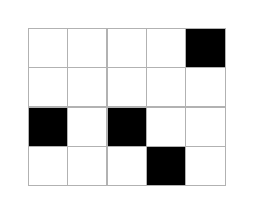
\begin{tikzpicture}[scale=0.5]
\foreach \r/\row in {0/00001,1/00010,2/10100,3/01000}{
  \foreach \c in {0,...,4}{
    \pgfmathsetmacro{\bit}{int(mod(floor(\row/10^(4-\c)),10))}
    \ifnum\bit=1 \fill[black] (\c,-\r) rectangle ++(1,1); \fi
    \draw[black!30] (\c,-\r) rectangle ++(1,1);}}
\end{tikzpicture}\end{center}
{\small\color{black!70} Coursework 2 Q2 is the same task on a bigger picture: 56 bits from fill (0,1,1,0,0,1) with a\textsubscript{n+6} = a\textsubscript{n+5} \ensuremath{\oplus} a\textsubscript{n}. Its stream begins 011001 101110 1101\ldots{}}\par
\end{example}
\subsection*{3.2 Periods, the companion matrix and the Main Theorem}\addcontentsline{toc}{subsection}{3.2 Periods, the companion matrix and the Main Theorem}\label{ch3-period}
\begin{concept}{Facts to know (state them; no proofs needed)}
\begin{itemize}
\item \textbf{Period} Per(a\textsubscript{0}): the smallest j \ensuremath{\ge} 1 with a\textsubscript{i+j} = a\textsubscript{i} for some i. Bigger is better.
\item The zero fill gives 000\ldots{} with Per = 1: a useless key (it encrypts nothing).
\item \textbf{Per(a\textsubscript{0}) \ensuremath{\le} 2\textsuperscript{n} \ensuremath{-} 1} for every fill (pigeonhole: only 2\textsuperscript{n} \ensuremath{-} 1 non-zero states).
\item If \textbf{b\textsubscript{0} = 0}, the first bit is never used. The LFSR is really a shorter one: s = a\textsubscript{0}\ldots{}a\textsubscript{k\ensuremath{-}1}s′, where s′ comes from the LFSR with taps (b\textsubscript{k}, \ldots{}, b\textsubscript{n\ensuremath{-}1}) and fill (a\textsubscript{k}, \ldots{}, a\textsubscript{n\ensuremath{-}1}) (Lemma 3.10). So assume b\textsubscript{0} = 1.
\item If \textbf{b\textsubscript{0} = 1}: the period is the first j with \textbf{a\textsubscript{j} = a\textsubscript{0}} (the fill itself comes back), and Per(a\textsubscript{0}) divides ord(B\textsubscript{b}).
\end{itemize}
\end{concept}
\begin{concept}{Companion matrix and characteristic polynomial}
a\textsubscript{i+1} = a\textsubscript{i}B\textsubscript{b}, where B\textsubscript{b} has 1s just below the diagonal and the taps down the last column. For b = (1, 0, 1, 1):\par
\ensuremath{\begin{pmatrix}0&0&0&1\\1&0&0&0\\0&1&0&1\\0&0&1&1\end{pmatrix}}\par
Here B\textsubscript{b}\textsuperscript{7} = I, so every period divides 7: it is 1 or 7.\par
The \textbf{characteristic polynomial} is \textbf{c\textsubscript{b}(x) = x\textsuperscript{n} + b\textsubscript{n\ensuremath{-}1}x\textsuperscript{n\ensuremath{-}1} + \ldots{} + b\textsubscript{1}x + b\textsubscript{0}} \ensuremath{\in} F\textsubscript{2}[x]. Quick rule: replace a\textsubscript{i+k} by x\textsuperscript{k} in the update rule and add the left-hand side. For a\textsubscript{i+5} = a\textsubscript{i+2} \ensuremath{\oplus} a\textsubscript{i}, c\textsubscript{b}(x) = x\textsuperscript{5} + x\textsuperscript{2} + 1.\par
\end{concept}
\begin{concept}{The Main Theorem (Theorem 3.16)}
If c\textsubscript{b}(x) is \textbf{irreducible}, then every \textbf{non-zero} initial fill has the \textbf{same} period j, where j is the \textbf{smallest divisor of 2\textsuperscript{n} \ensuremath{-} 1} with c\textsubscript{b}(x) | x\textsuperscript{j} + 1.\par
\end{concept}
\begin{method}{Method: find the period with the Main Theorem}
\begin{enumerate}[label=\protect\stepnum{\arabic*}, leftmargin=2.2em]
\item Write down c\textsubscript{b}(x).
\item \textbf{Prove it is irreducible} (table below). A polynomial of degree n is reducible exactly when it has an irreducible factor of degree \ensuremath{\le} n/2.
\item List the divisors of 2\textsuperscript{n} \ensuremath{-} 1 in increasing order.
\item Skip any j < n: a degree-n polynomial cannot divide x\textsuperscript{j} + 1 of smaller degree.
\item Test the remaining divisors in order by long division (or a known factorisation). The first j that works is the period. If 2\textsuperscript{n} \ensuremath{-} 1 is prime (n = 2, 3, 5, 7), the period is 2\textsuperscript{n} \ensuremath{-} 1 straight away.
\item State the conclusion: "Per(a\textsubscript{0}) = j for every non-zero fill a\textsubscript{0}; the zero fill has period 1."
\end{enumerate}
\end{method}
\begin{xltabular}{\linewidth}{|l|>{\raggedright\arraybackslash}X|}\hline
\rowcolor{navy!10}\textbf{Degree of c\textsubscript{b}} & \textbf{To prove irreducible, check\ldots{}} \\ \hline\endhead
2 or 3 & No roots: c(0) = 1 (constant term 1) and c(1) = 1 (odd number of terms) \\ \hline
4 or 5 & No roots, \textbf{and} not divisible by x\textsuperscript{2} + x + 1. For degree 4 this means c \ensuremath{\neq} (x\textsuperscript{2} + x + 1)\textsuperscript{2} = x\textsuperscript{4} + x\textsuperscript{2} + 1 \\ \hline
6 & No roots, not divisible by x\textsuperscript{2} + x + 1, x\textsuperscript{3} + x + 1 or x\textsuperscript{3} + x\textsuperscript{2} + 1 \\ \hline
\end{xltabular}
{\small\color{black!70} Irreducible polynomials over F\textsubscript{2} up to degree 4: x, x + 1; x\textsuperscript{2} + x + 1; x\textsuperscript{3} + x + 1, x\textsuperscript{3} + x\textsuperscript{2} + 1; x\textsuperscript{4} + x + 1, x\textsuperscript{4} + x\textsuperscript{3} + 1, x\textsuperscript{4} + x\textsuperscript{3} + x\textsuperscript{2} + x + 1.}\par
\begin{example}{Worked example: Coursework 2 Q3, rule a\textsubscript{n+5} = a\textsubscript{n+2} \ensuremath{\oplus} a\textsubscript{n}}
\textbf{(a)} Taps b = (1, 0, 1, 0, 0), so c\textsubscript{b}(x) = x\textsuperscript{5} + x\textsuperscript{2} + 1.\par
No roots: c\textsubscript{b}(0) = 1 and c\textsubscript{b}(1) = 1 + 1 + 1 = 1. So there is no linear factor. A reducible quintic would need a factor of degree 1 or 2, and the only irreducible quadratic is x\textsuperscript{2} + x + 1. Divide:\par
\begin{workbox}
\begin{Verbatim}[commandchars=\\\{\},fontsize=\footnotesize]
x\textsuperscript{5} + x\textsuperscript{2} + 1  −  x\textsuperscript{3}(x\textsuperscript{2} + x + 1)  =  x\textsuperscript{4} + x\textsuperscript{3} + x\textsuperscript{2} + 1
x\textsuperscript{4} + x\textsuperscript{3} + x\textsuperscript{2} + 1  −  x\textsuperscript{2}(x\textsuperscript{2} + x + 1)  =  1
Remainder 1 ≠ 0, so x\textsuperscript{2} + x + 1 does not divide c\textsubscript{b}(x).
\end{Verbatim}
\end{workbox}
Hence c\textsubscript{b}(x) is irreducible.\par
\textbf{(b)} By the Main Theorem, the period divides 2\textsuperscript{5} \ensuremath{-} 1 = 31, which is prime, so it is 1 or 31. It is not 1, since c\textsubscript{b} (degree 5) cannot divide x + 1. So \textbf{Per(a\textsubscript{0}) = 31 for every non-zero fill}, the maximum possible.\par
\end{example}
\begin{example}{Worked example (2025 paper): c\textsubscript{b}(x) = x\textsuperscript{4} + x + 1}
Irreducible: c(0) = 1, c(1) = 1 + 1 + 1 = 1, and c \ensuremath{\neq} x\textsuperscript{4} + x\textsuperscript{2} + 1 = (x\textsuperscript{2} + x + 1)\textsuperscript{2}. Divisors of 15: 1, 3, 5, 15. Skip 1 and 3 (smaller than 4). Test 5:\par
\begin{workbox}
\begin{Verbatim}[commandchars=\\\{\},fontsize=\footnotesize]
x\textsuperscript{5} + 1 − x(x\textsuperscript{4} + x + 1) = x\textsuperscript{2} + x + 1 ≠ 0,  so c ∤ x\textsuperscript{5} + 1.
\end{Verbatim}
\end{workbox}
So the period is \textbf{15} for every non-zero fill (maximal). Check: fill 1011 gives s = 101111000100110 1011\ldots{}, which repeats after 15 bits.\par
\end{example}
\begin{trap}{When the theorem does not apply: a reducible polynomial}
For b = (1, 0, 1, 0), c\textsubscript{b}(x) = x\textsuperscript{4} + x\textsuperscript{2} + 1 = (x\textsuperscript{2} + x + 1)\textsuperscript{2} is reducible. Then different fills can have different periods, which need not divide 15. With a\textsubscript{i+4} = a\textsubscript{i} \ensuremath{\oplus} a\textsubscript{i+2}:\par
\begin{workbox}
\begin{Verbatim}[commandchars=\\\{\},fontsize=\footnotesize]
fill 0110:  0110 110 110 …     period 3
fill 1000:  100010 100010 …    period 6   (6 does not divide 15)
\end{Verbatim}
\end{workbox}
{\small\color{black!70} Note: the strings printed in the notes' Example 3.17(3) do not follow the stated update rule (a period-2 output is impossible for this rule). The periods above are the correct ones. The lesson is unchanged.}\par
\end{trap}
\begin{tip}{Exam tip: no roots is not enough}
x\textsuperscript{4} + x\textsuperscript{2} + 1 has no roots in F\textsubscript{2} but is reducible. For degree 4 or 5, always also rule out x\textsuperscript{2} + x + 1 as a factor. Also, irreducible does \textbf{not} mean maximal period: x\textsuperscript{4} + x\textsuperscript{3} + x\textsuperscript{2} + x + 1 is irreducible but divides x\textsuperscript{5} + 1, so its period is only 5.\par
\end{tip}
\subsection*{Chapters 2–3 practice questions}\addcontentsline{toc}{subsection}{Chapters 2–3 practice questions}\label{ch3-q}
\begin{question}{\lvleasy{}2.1 Enigma components\hfill\textnormal{\small [4]}}
Briefly describe the role of the plugboard, rotors and reflector in the Enigma machine, and explain why the same settings can be used to decrypt.\par
\end{question}
\begin{answer}
\textbf{Plugboard:} cables swap fixed pairs of letters, a substitution applied when the signal enters and leaves. \textbf{Rotors:} three wired wheels, each permuting the alphabet; the right rotor steps after every key press (middle every 26 steps, left every 26² steps), so the substitution changes with every letter. \textbf{Reflector:} pairs all 26 letters and sends the signal back through the rotors and plugboard in reverse.\par
Overall \ensuremath{\sigma}\textsubscript{i} = P\textsuperscript{\ensuremath{-}1}R\textsuperscript{\ensuremath{-}1}SRP (rotors combined into R) is a conjugate of S, so it swaps letters in pairs and \ensuremath{\sigma}\textsubscript{i} = \ensuremath{\sigma}\textsubscript{i}\textsuperscript{\ensuremath{-}1}. Typing the ciphertext with the same settings therefore gives back the plaintext.\par
\end{answer}
\begin{question}{\lvlmed{}2.2 Counting settings\hfill\textnormal{\small [3]}}
A simplified Enigma has a 10-letter alphabet, uses 3 rotors chosen (in order) from 4, uses exactly 2 plugs, and has a choice of 2 reflectors. How many settings are there?\par
\end{question}
\begin{answer}
\begin{workbox}
\begin{Verbatim}[commandchars=\\\{\},fontsize=\footnotesize]
Plugboard: C(10,4)·3·1 = 210·3 = 630
Rotors in order: 4·3·2 = 24;  starting positions: 10\textsuperscript{3} = 1 000
Reflectors: 2
Total = 630 × 24 × 1 000 × 2 = 30 240 000
\end{Verbatim}
\end{workbox}
\end{answer}
\begin{question}{\lvlhard{}2.3 Counting with "up to"\hfill\textnormal{\small [3]}}
(a) With a 6-letter alphabet, how many plugboard settings use \textbf{up to} 2 plugs? (b) With an 8-letter alphabet, how many different reflector wirings are possible?\par
\end{question}
\begin{answer}
\begin{workbox}
\begin{Verbatim}[commandchars=\\\{\},fontsize=\footnotesize]
(a) 0 plugs: 1
    1 plug:  C(6,2)·1   = 15
    2 plugs: C(6,4)·3·1 = 45
    Total = 1 + 15 + 45 = 61
(b) A reflector pairs all 8 letters: C(8,8)·7·5·3·1 = 105
\end{Verbatim}
\end{workbox}
\end{answer}
\begin{question}{\lvleasy{}3.1 Generate and encrypt\hfill\textnormal{\small [4]}}
An LFSR has update rule a\textsubscript{i+3} = a\textsubscript{i} \ensuremath{\oplus} a\textsubscript{i+1} and initial fill 100. (a) Write down the first 8 output bits. (b) Encrypt the letter A (ASCII 01000001). (c) Find the period of this fill.\par
\end{question}
\begin{answer}
\begin{workbox}
\begin{Verbatim}[commandchars=\\\{\},fontsize=\footnotesize]
a\textsubscript{3} = a\textsubscript{0} ⊕ a\textsubscript{1} = 1 ⊕ 0 = 1      a\textsubscript{6} = a\textsubscript{3} ⊕ a\textsubscript{4} = 1 ⊕ 0 = 1
a\textsubscript{4} = a\textsubscript{1} ⊕ a\textsubscript{2} = 0 ⊕ 0 = 0      a\textsubscript{7} = a\textsubscript{4} ⊕ a\textsubscript{5} = 0 ⊕ 1 = 1
a\textsubscript{5} = a\textsubscript{2} ⊕ a\textsubscript{3} = 0 ⊕ 1 = 1
(a) s = 1 0 0 1 0 1 1 1 …
(b) m = 0 1 0 0 0 0 0 1
    s = 1 0 0 1 0 1 1 1
    c = 1 1 0 1 0 1 1 0
\end{Verbatim}
\end{workbox}
(c) Continuing, s = 1001011 1001011\ldots{}, and the state 100 first returns at a\textsubscript{7}, so Per = 7. Check with the theorem: c\textsubscript{b}(x) = x\textsuperscript{3} + x + 1 has no roots, so it is irreducible, and 2\textsuperscript{3} \ensuremath{-} 1 = 7 is prime, so the period is 7 for every non-zero fill.\par
\end{answer}
\begin{question}{\lvlmed{}3.2 Main Theorem\hfill\textnormal{\small [5]}}
An LFSR has update rule a\textsubscript{i+4} = a\textsubscript{i+3} \ensuremath{\oplus} a\textsubscript{i}. Write down its taps and characteristic polynomial, show the polynomial is irreducible, and find the period of every non-zero fill. (You may use that x\textsuperscript{2} + x + 1 is the only irreducible quadratic over F\textsubscript{2}.)\par
\end{question}
\begin{answer}
Taps b = (1, 0, 0, 1), so c\textsubscript{b}(x) = x\textsuperscript{4} + x\textsuperscript{3} + 1.\par
c(0) = 1, c(1) = 1 + 1 + 1 = 1: no roots, so no linear factors. A reducible quartic without linear factors would be a product of two irreducible quadratics, i.e. (x\textsuperscript{2} + x + 1)\textsuperscript{2} = x\textsuperscript{4} + x\textsuperscript{2} + 1 \ensuremath{\neq} c(x). So c is irreducible.\par
Divisors of 2\textsuperscript{4} \ensuremath{-} 1 = 15: 1, 3, 5, 15. Skip 1 and 3. Test 5:\par
\begin{workbox}
\begin{Verbatim}[commandchars=\\\{\},fontsize=\footnotesize]
x\textsuperscript{5} + 1 − x(x\textsuperscript{4} + x\textsuperscript{3} + 1) = x\textsuperscript{4} + x + 1
x\textsuperscript{4} + x + 1 − (x\textsuperscript{4} + x\textsuperscript{3} + 1) = x\textsuperscript{3} + x ≠ 0
\end{Verbatim}
\end{workbox}
So c \ensuremath{\nmid} x\textsuperscript{5} + 1, and by the Main Theorem \textbf{Per(a\textsubscript{0}) = 15} for every non-zero fill.\par
\end{answer}
\begin{question}{\lvlmed{}3.3 Irreducible but not maximal\hfill\textnormal{\small [3]}}
For taps b = (1, 1, 1, 1), find the period of every non-zero fill, given x\textsuperscript{5} + 1 = (x + 1)(x\textsuperscript{4} + x\textsuperscript{3} + x\textsuperscript{2} + x + 1).\par
\end{question}
\begin{answer}
c\textsubscript{b}(x) = x\textsuperscript{4} + x\textsuperscript{3} + x\textsuperscript{2} + x + 1. c(0) = 1 and c(1) = 5 terms = 1, so no roots, and c \ensuremath{\neq} x\textsuperscript{4} + x\textsuperscript{2} + 1, so it is irreducible. Divisors of 15: skip 1 and 3; c divides x\textsuperscript{5} + 1 by the given factorisation. So \textbf{Per = 5} for every non-zero fill. Example: fill 1001 gives 10010 10010\ldots{}\par
\end{answer}
\begin{question}{\lvlhard{}3.4 Degree 6\hfill\textnormal{\small [6]}}
Show that c(x) = x\textsuperscript{6} + x\textsuperscript{3} + 1 is irreducible over F\textsubscript{2} and find the period of a non-zero fill for the corresponding LFSR (taps (1, 0, 0, 1, 0, 0)).\par
\end{question}
\begin{answer}
\textbf{Irreducible.} c(0) = 1 and c(1) = 1 (three terms): no linear factor. Any other factorisation would include an irreducible factor of degree 2 or 3. Long division gives:\par
\begin{workbox}
\begin{Verbatim}[commandchars=\\\{\},fontsize=\footnotesize]
c(x) mod (x\textsuperscript{2} + x + 1)     = 1
c(x) mod (x\textsuperscript{3} + x + 1)     = x\textsuperscript{2} + x + 1
c(x) mod (x\textsuperscript{3} + x\textsuperscript{2} + 1) = x
\end{Verbatim}
\end{workbox}
None is 0, so c is irreducible. (Quick check for the first: x\textsuperscript{3} \ensuremath{\equiv} 1 mod x\textsuperscript{2} + x + 1, so c \ensuremath{\equiv} 1 + 1 + 1 = 1.)\par
\textbf{Period.} Divisors of 63: 1, 3, 7, 9, 21, 63. Skip 1 and 3 (less than 6). Test 7: x\textsuperscript{7} + 1 \ensuremath{\equiv} x\textsuperscript{4} + x + 1 (mod c), not 0. Test 9: x\textsuperscript{9} + 1 = (x\textsuperscript{3} + 1)(x\textsuperscript{6} + x\textsuperscript{3} + 1), so c | x\textsuperscript{9} + 1. Hence \textbf{Per = 9}, far below the maximum 63. Irreducible guarantees equal periods, not maximal ones.\par
\end{answer}
\begin{question}{\lvlunseen{}3.5 First tap zero\hfill\textnormal{\small [3]}}
An LFSR has rule a\textsubscript{i+4} = a\textsubscript{i+1} \ensuremath{\oplus} a\textsubscript{i+3}. Find the period of fill 1001 and of fill 1000 without generating many bits.\par
\end{question}
\begin{answer}
Taps (0, 1, 0, 1): b\textsubscript{0} = 0, so a\textsubscript{i} is never used. By Lemma 3.10, after the first bit the output is that of the length-3 LFSR with taps (1, 0, 1) (rule a\textsubscript{i+3} = a\textsubscript{i} \ensuremath{\oplus} a\textsubscript{i+2}) and fill (a\textsubscript{1}, a\textsubscript{2}, a\textsubscript{3}). Its polynomial x\textsuperscript{3} + x\textsuperscript{2} + 1 has no roots, so it is irreducible, and 7 is prime.\par
\begin{itemize}
\item Fill 1001: reduced fill 001 \ensuremath{\neq} 0, so \textbf{Per = 7} (s = 1 0011101 0011101\ldots{}).
\item Fill 1000: reduced fill 000, so s = 1 000000\ldots{}, \textbf{Per = 1}.
\end{itemize}
\end{answer}
\begin{question}{\lvlunseen{}3.6 Security of an LFSR stream\hfill\textnormal{\small [3]}}
Eve knows that a message was encrypted with an LFSR of length 5 whose taps she knows, and she knows the first 5 plaintext bits. Explain why the whole message is exposed.\par
\end{question}
\begin{answer}
XORing the known plaintext bits with the ciphertext bits gives s\textsubscript{i} = c\textsubscript{i} \ensuremath{\oplus} m\textsubscript{i} for i = 0, \ldots{}, 4. These are exactly the initial fill. With the known update rule Eve regenerates the entire stream and decrypts everything. The output is deterministic, not random, so an LFSR does not have the One Time Pad's perfect security. (Even with unknown taps, about 2n known bits give enough linear equations to find them.)\par
\end{answer}
\guidesection{Chapter 4 \ensuremath{\cdot} Exam Q3}{Public key cryptography}\label{ch4}
\textbf{The big picture.} Classical ciphers need a shared secret key. Public key cryptography is \textbf{asymmetric}: some information is public, some private, and an attacker would have to solve a \textbf{hard mathematical problem} to break it.\par
\begin{xltabular}{\linewidth}{|l|>{\raggedright\arraybackslash}X|>{\raggedright\arraybackslash}X|}\hline
\rowcolor{navy!10}\textbf{Scheme} & \textbf{Purpose} & \textbf{Hard problem protecting it} \\ \hline\endhead
Diffie–Hellman & Agree a shared key without sending it & Diffie–Hellman Problem / Discrete Log Problem \\ \hline
RSA & Encryption, signatures & RSA Problem / Semiprime Factorisation Problem \\ \hline
El-Gamal & Encryption, signatures & Discrete Log Problem in the chosen group G \\ \hline
\end{xltabular}
\subsection*{4.1 Primitive roots and Diffie–Hellman key exchange}\addcontentsline{toc}{subsection}{4.1 Primitive roots and Diffie–Hellman key exchange}
\begin{concept}{Primitive roots}
(Z/pZ)\textsuperscript{\ensuremath{\times}} = \{1, \ldots{}, p \ensuremath{-} 1\} is cyclic. g is a \textbf{primitive root} if every element is a power of g, i.e. g has order p \ensuremath{-} 1.\par
\textbf{Quick test:} g is a primitive root mod p if and only if g\textsuperscript{(p\ensuremath{-}1)/q} \ensuremath{\not\equiv} 1 for every prime q dividing p \ensuremath{-} 1. (You can also list powers, as the notes do.)\par
\end{concept}
\begin{example}{Worked example: is 5 a primitive root mod 23?}
\begin{workbox}
\begin{Verbatim}[commandchars=\\\{\},fontsize=\footnotesize]
p − 1 = 22 = 2·11. Check 5\textsuperscript{22/2} = 5\textsuperscript{11} and 5\textsuperscript{22/11} = 5\textsuperscript{2}.
5\textsuperscript{2} = 25 ≡ 2 ≠ 1
5\textsuperscript{4} ≡ 4, 5\textsuperscript{8} ≡ 16, 5\textsuperscript{11} = 5\textsuperscript{8}·5\textsuperscript{2}·5 ≡ 16·2·5 = 160 ≡ 22 ≡ −1 ≠ 1
So 5 is a primitive root mod 23.
\end{Verbatim}
\end{workbox}
By contrast 2 is not a primitive root mod 7: 2\textsuperscript{3} = 8 \ensuremath{\equiv} 1, so its powers are only 2, 4, 1.\par
\end{example}
\begin{method}{Diffie–Hellman key exchange \guidetag{memo}{memorise}}
\begin{enumerate}[label=\protect\stepnum{\arabic*}, leftmargin=2.2em]
\item Alice and Bob publicly agree a prime p and a primitive root g \ensuremath{\in} (Z/pZ)\textsuperscript{\ensuremath{\times}}.
\item Alice picks a private k\textsubscript{A} and sends c\textsubscript{A} = g\textsuperscript{k\textsubscript{A}} to Bob.
\item Bob picks a private k\textsubscript{B} and sends c\textsubscript{B} = g\textsuperscript{k\textsubscript{B}} to Alice.
\item Alice computes c\textsubscript{B}\textsuperscript{k\textsubscript{A}}, Bob computes c\textsubscript{A}\textsuperscript{k\textsubscript{B}}. Both equal \textbf{g\textsuperscript{k\textsubscript{A}k\textsubscript{B}}}, the shared key.
\end{enumerate}
\end{method}
\begin{example}{Worked example: p = 23, g = 5, k\textsubscript{A} = 6, k\textsubscript{B} = 15}
\begin{workbox}
\begin{Verbatim}[commandchars=\\\{\},fontsize=\footnotesize]
Powers of 5 mod 23:  5\textsuperscript{2} ≡ 2,  5\textsuperscript{4} ≡ 4,  5\textsuperscript{8} ≡ 16
c\textsubscript{A} = 5\textsuperscript{6}  = 5\textsuperscript{4}·5\textsuperscript{2} ≡ 4·2 = 8
c\textsubscript{B} = 5\textsuperscript{15} = 5\textsuperscript{8}·5\textsuperscript{4}·5\textsuperscript{2}·5 ≡ 16·4·2·5 = 640 ≡ 640 − 27·23 = 19
Alice: 19\textsuperscript{6} ≡ (−4)\textsuperscript{6}.  (−4)\textsuperscript{2} = 16,  (−4)\textsuperscript{4} = 256 ≡ 3,  (−4)\textsuperscript{6} ≡ 3·16 = 48 ≡ 2
Bob:   8\textsuperscript{15}.  8\textsuperscript{2} = 64 ≡ −5,  8\textsuperscript{4} ≡ 25 ≡ 2,  8\textsuperscript{8} ≡ 4
       8\textsuperscript{15} = 8\textsuperscript{8}·8\textsuperscript{4}·8\textsuperscript{2}·8 ≡ 4·2·(−5)·8 = −320 ≡ −320 + 14·23 = 2
Shared key: 2 ✓ (both agree)
\end{Verbatim}
\end{workbox}
\end{example}
\begin{concept}{Security: what Eve faces}
Eve knows p, g, g\textsuperscript{k\textsubscript{A}}, g\textsuperscript{k\textsubscript{B}}. \textbf{Diffie–Hellman Problem:} from g\textsuperscript{x} and g\textsuperscript{y}, find g\textsuperscript{xy}. If she could solve the \textbf{Discrete Log Problem} (given p, g, h, find x = dlog\textsubscript{g}(h) with g\textsuperscript{x} = h), she could recover k\textsubscript{A} and then the key. dlog\textsubscript{g}(h) is only defined mod p \ensuremath{-} 1. For large p (600–700 digits) the best known algorithms are sub-exponential, so this is infeasible.\par
Example: 2 is a primitive root mod 11 with powers 2, 4, 8, 5, 10, 9, 7, 3, 6, 1, so dlog\textsubscript{2}(3) = 8 and dlog\textsubscript{2}(10) = 5.\par
\end{concept}
\subsection*{4.2 RSA}\addcontentsline{toc}{subsection}{4.2 RSA}\label{ch4-rsa}
\begin{concept}{Background}
(Z/NZ)\textsuperscript{\ensuremath{\times}} = \{a : gcd(a, N) = 1\}; \ensuremath{\varphi}(N) = |(Z/NZ)\textsuperscript{\ensuremath{\times}}|; for distinct primes, \textbf{\ensuremath{\varphi}(pq) = (p \ensuremath{-} 1)(q \ensuremath{-} 1)}. \textbf{Fermat–Euler:} a\textsuperscript{\ensuremath{\varphi}(N)} \ensuremath{\equiv} 1 (mod N) when gcd(a, N) = 1. So if ed \ensuremath{\equiv} 1 (mod \ensuremath{\varphi}(N)), then (m\textsuperscript{e})\textsuperscript{d} = m\textsuperscript{1 + k\ensuremath{\varphi}(N)} = m: the maps f\textsubscript{e}(m) = m\textsuperscript{e} and f\textsubscript{d} are inverse to each other.\par
\end{concept}
\begin{method}{RSA encryption and decryption \guidetag{memo}{memorise}}
\begin{enumerate}[label=\protect\stepnum{\arabic*}, leftmargin=2.2em]
\item \textbf{Key generation (Alice):} secret distinct primes p, q; N = pq; choose e with gcd(e, (p \ensuremath{-} 1)(q \ensuremath{-} 1)) = 1.
\item \textbf{Public key} (N, e). \textbf{Private key} (p, q, d), where d \ensuremath{\equiv} e\textsuperscript{\ensuremath{-}1} (mod (p \ensuremath{-} 1)(q \ensuremath{-} 1)), found by Extended Euclid.
\item \textbf{Encrypt (Bob):} c \ensuremath{\equiv} m\textsuperscript{e} (mod N).
\item \textbf{Decrypt (Alice):} m \ensuremath{\equiv} c\textsuperscript{d} (mod N).
\end{enumerate}
\end{method}
\begin{example}{Worked example: Coursework 3 Q1, (N, e) = (299, 5), m = 10}
\textbf{Encrypt.}\par
\begin{workbox}
\begin{Verbatim}[commandchars=\\\{\},fontsize=\footnotesize]
10\textsuperscript{2} = 100
10\textsuperscript{4} = 100\textsuperscript{2} = 10 000 = 33·299 + 133 ≡ 133
c = 10\textsuperscript{5} = 10\textsuperscript{4}·10 ≡ 1330 = 4·299 + 134 ≡ 134
\end{Verbatim}
\end{workbox}
\textbf{Decrypt.} Alice knows 299 = 13 \ensuremath{\cdot} 23, so \ensuremath{\varphi}(N) = 12 \ensuremath{\cdot} 22 = 264. From the toolkit, d = 5\textsuperscript{\ensuremath{-}1} mod 264 = 53. Now compute 134\textsuperscript{53} mod 299 with 53 = 32 + 16 + 4 + 1:\par
\begin{workbox}
\begin{Verbatim}[commandchars=\\\{\},fontsize=\footnotesize]
c\textsuperscript{1}  = 134
c\textsuperscript{2}  = 17 956 ≡ 16
c\textsuperscript{4}  = 256
c\textsuperscript{8}  = 65 536 ≡ 55
c\textsuperscript{16} = 3 025 ≡ 35
c\textsuperscript{32} = 1 225 ≡ 29
c\textsuperscript{53} = c\textsuperscript{32}·c\textsuperscript{16}·c\textsuperscript{4}·c ≡ 29·35·256·134
      29·35 = 1015 ≡ 118;  118·256 = 30 208 ≡ 9;  9·134 = 1206 ≡ 10
m = 10 ✓
\end{Verbatim}
\end{workbox}
\end{example}
\begin{concept}{Security}
\textbf{RSA Problem:} from (N, e) and c = m\textsuperscript{e}, recover m. The only known route is to find d, which needs \ensuremath{\varphi}(N) = (p \ensuremath{-} 1)(q \ensuremath{-} 1), which needs p and q. So RSA is broken by the \textbf{Semiprime Factorisation Problem}: given N = pq, find p, q. Real primes are 300–400 digits; the best factoring algorithms are sub-exponential, too slow at that size.\par
\end{concept}
\subsection*{4.3 El-Gamal encryption}\addcontentsline{toc}{subsection}{4.3 El-Gamal encryption}\label{ch4-eg}
\guidetag{sheet}{on the Useful Information sheet}\par
\begin{method}{El-Gamal}
\begin{enumerate}[label=\protect\stepnum{\arabic*}, leftmargin=2.2em]
\item \textbf{Key generation (Alice):} finite cyclic group G of size q with generator g; secret 1 \ensuremath{\le} k \ensuremath{\le} q; h = g\textsuperscript{k}. Public key (G, q, g, h); private key k.
\item \textbf{Encrypt (Bob):} choose a secret 1 \ensuremath{\le} s \ensuremath{\le} q; send c\textsubscript{1} = g\textsuperscript{s}, c\textsubscript{2} = m\ensuremath{\cdot}h\textsuperscript{s}.
\item \textbf{Decrypt (Alice):} m = c\textsubscript{2}\ensuremath{\cdot}c\textsubscript{1}\textsuperscript{\ensuremath{-}k}. (It works because c\textsubscript{1}\textsuperscript{k} = g\textsuperscript{sk} = h\textsuperscript{s}.)
\end{enumerate}
\end{method}
\begin{example}{Worked example: G = (Z/23Z)\textsuperscript{\ensuremath{\times}}, q = 22, g = 5, k = 6, m = 10, s = 3}
\begin{workbox}
\begin{Verbatim}[commandchars=\\\{\},fontsize=\footnotesize]
Public key: h = 5\textsuperscript{6} ≡ 8, so (G, q, g, h) = (G, 22, 5, 8)
Encrypt:  c\textsubscript{1} = 5\textsuperscript{3} = 125 ≡ 10
          h\textsuperscript{3} = 512 ≡ 6,  c\textsubscript{2} = 10·6 = 60 ≡ 14        send (10, 14)
Decrypt:  c\textsubscript{1}\textsuperscript{k} = 10\textsuperscript{6}:  10\textsuperscript{2} ≡ 8, 10\textsuperscript{4} ≡ 64 ≡ −5, 10\textsuperscript{6} ≡ 8·(−5) = −40 ≡ 6
          6\textsuperscript{−1} ≡ 4 (since 6·4 = 24 ≡ 1)
          m = 14·4 = 56 ≡ 10 ✓
\end{Verbatim}
\end{workbox}
Alternative: c\textsubscript{1}\textsuperscript{\ensuremath{-}k} = c\textsubscript{1}\textsuperscript{q\ensuremath{-}k} = 10\textsuperscript{16}, which avoids computing an inverse.\par
\end{example}
\begin{concept}{Security and choice of group}
Eve sees G, q, g, h, c\textsubscript{1}, c\textsubscript{2}. To get m she needs k = dlog\textsubscript{g}(h): the Discrete Log Problem in G. \textbf{The presentation of G matters.} In G = Z/NZ under addition, "g\textsuperscript{k}" means kg, so the DLP is just kg \ensuremath{\equiv} h (mod N), solved instantly by k \ensuremath{\equiv} g\textsuperscript{\ensuremath{-}1}h (e.g. dlog\textsubscript{7}(9) = 5 in Z/13Z, since 7\textsuperscript{\ensuremath{-}1}\ensuremath{\cdot}9 \ensuremath{\equiv} 2\ensuremath{\cdot}9 = 18 \ensuremath{\equiv} 5). Never use an additive group. (Z/pZ)\textsuperscript{\ensuremath{\times}} and elliptic curve groups E(F\textsubscript{p}) are good choices. q is included in the public key because |G| may not be obvious.\par
\end{concept}
\subsection*{4.4 Digital signatures}\addcontentsline{toc}{subsection}{4.4 Digital signatures}\label{ch4-sig}
A signature proves the sender knows their private key \textbf{without revealing it}. The signer uses their \textbf{own private key}. The receiver verifies with the \textbf{signer's public key}.\par
\begin{method}{RSA signatures \guidetag{memo}{memorise}}
\begin{enumerate}[label=\protect\stepnum{\arabic*}, leftmargin=2.2em]
\item Alice has public (N, e) and private d.
\item Given an auxiliary message m\textsubscript{0} \ensuremath{\in} (Z/NZ)\textsuperscript{\ensuremath{\times}} (a challenge from Bob, or in practice a hash H(m)), Alice computes \textbf{m\textsubscript{1} = m\textsubscript{0}\textsuperscript{d} mod N} and sends (m\textsubscript{0}, m\textsubscript{1}) alongside her message (which is encrypted with \textbf{Bob's} public key).
\item Bob verifies with Alice's public key: \textbf{m\textsubscript{1}\textsuperscript{e} \ensuremath{\equiv} m\textsubscript{0} (mod N)?}
\end{enumerate}
\end{method}
\begin{example}{Worked example (2025 paper): (N, e) = (33, 3), d = 7, m\textsubscript{0} = 14}
\begin{workbox}
\begin{Verbatim}[commandchars=\\\{\},fontsize=\footnotesize]
ϕ(33) = 2·10 = 20 and 3·7 = 21 ≡ 1, so d = 7.
Sign:   14\textsuperscript{2} = 196 ≡ 31 ≡ −2,  14\textsuperscript{4} ≡ 4
        m\textsubscript{1} = 14\textsuperscript{7} = 14\textsuperscript{4}·14\textsuperscript{2}·14 ≡ 4·(−2)·14 = −112 ≡ 20
Verify: 20\textsuperscript{3} = 8000 = 242·33 + 14 ≡ 14 = m\textsubscript{0} ✓        Signature (14, 20)
\end{Verbatim}
\end{workbox}
\end{example}
\begin{method}{El-Gamal signatures \guidetag{sheet}{on the sheet} (G = (Z/pZ)\textsuperscript{\ensuremath{\times}}, q = p \ensuremath{-} 1)}
\begin{enumerate}[label=\protect\stepnum{\arabic*}, leftmargin=2.2em]
\item Alice has public (G, q, g, h = g\textsuperscript{k}) and private k.
\item She picks an auxiliary message m\textsubscript{0} and a secret s with \textbf{gcd(s, q) = 1} (so s\textsuperscript{\ensuremath{-}1} mod q exists).
\item \textbf{m\textsubscript{1} = g\textsuperscript{s} mod p} and \textbf{m\textsubscript{2} \ensuremath{\equiv} (m\textsubscript{0} \ensuremath{-} k\ensuremath{\cdot}m\textsubscript{1})\ensuremath{\cdot}s\textsuperscript{\ensuremath{-}1} (mod q)}. Note: m\textsubscript{2} is an exponent, so it is computed mod q = p \ensuremath{-} 1.
\item She sends (m\textsubscript{0}, m\textsubscript{1}, m\textsubscript{2}). Bob checks \textbf{h\textsuperscript{m\textsubscript{1}}\ensuremath{\cdot}m\textsubscript{1}\textsuperscript{m\textsubscript{2}} \ensuremath{\equiv} g\textsuperscript{m\textsubscript{0}} (mod p)}.
\end{enumerate}
{\small\color{black!70} Why it works: h\textsuperscript{m\textsubscript{1}}m\textsubscript{1}\textsuperscript{m\textsubscript{2}} = g\textsuperscript{km\textsubscript{1} + sm\textsubscript{2}} = g\textsuperscript{km\textsubscript{1} + (m\textsubscript{0} \ensuremath{-} km\textsubscript{1})} = g\textsuperscript{m\textsubscript{0}}.}\par
\end{method}
\begin{example}{Worked example: Coursework 3 Q2. p = 89, (G, q, g, h) = (G, 88, 3, 66), k = 13, m\textsubscript{0} = 23, s = 5}
\begin{workbox}
\begin{Verbatim}[commandchars=\\\{\},fontsize=\scriptsize]
Step 1  m\textsubscript{1} = 3\textsuperscript{5} = 243 = 2·89 + 65 ≡ 65                  (mod p = 89)
Step 2  s\textsuperscript{−1}: 88 = 17·5 + 3, 5 = 3 + 2, 3 = 2 + 1  ⇒  5\textsuperscript{−1} ≡ 53 (mod 88)   [5·53 = 265 = 3·88 + 1]
Step 3  m\textsubscript{0} − k·m\textsubscript{1} = 23 − 13·65 = 23 − 845 = −822 ≡ −822 + 10·88 = 58   (mod q = 88)
        m\textsubscript{2} ≡ 58·53 = 3074 = 34·88 + 82 ≡ 82
Signature (m\textsubscript{0}, m\textsubscript{1}, m\textsubscript{2}) = (23, 65, 82)

Verify (mod 89):
 h\textsuperscript{m\textsubscript{1}} = 66\textsuperscript{65}:  66\textsuperscript{2}≡84, 66\textsuperscript{4}≡25, 66\textsuperscript{8}≡2, 66\textsuperscript{16}≡4, 66\textsuperscript{32}≡16, 66\textsuperscript{64}≡78
          66\textsuperscript{65} = 66\textsuperscript{64}·66 ≡ 78·66 = 5148 ≡ 75
 m\textsubscript{1}\textsuperscript{m\textsubscript{2}} = 65\textsuperscript{82}: 65\textsuperscript{2}≡42, 65\textsuperscript{4}≡73, 65\textsuperscript{8}≡78, 65\textsuperscript{16}≡32, 65\textsuperscript{32}≡45, 65\textsuperscript{64}≡67
          82 = 64 + 16 + 2:  65\textsuperscript{82} ≡ 67·32·42;  67·32 = 2144 ≡ 8;  8·42 = 336 ≡ 69
 LHS = 75·69 = 5175 ≡ 13
 g\textsuperscript{m\textsubscript{0}} = 3\textsuperscript{23}: 3\textsuperscript{2}=9, 3\textsuperscript{4}=81, 3\textsuperscript{8}≡64, 3\textsuperscript{16}≡2;  3\textsuperscript{23} = 3\textsuperscript{16}·3\textsuperscript{4}·3\textsuperscript{2}·3 ≡ 2·81·9·3 = 4374 ≡ 13
 LHS = RHS = 13 ✓
\end{Verbatim}
\end{workbox}
\end{example}
\begin{trap}{Common traps in signatures}
\begin{itemize}
\item Signing uses the \textbf{signer's} private key; verifying uses the \textbf{signer's} public key, not the receiver's.
\item In El-Gamal, m\textsubscript{1} is computed mod p but m\textsubscript{2} mod q = p \ensuremath{-} 1. Use the integer m\textsubscript{1} (e.g. 65) inside m\textsubscript{0} \ensuremath{-} km\textsubscript{1}.
\item s must be coprime to q, otherwise s\textsuperscript{\ensuremath{-}1} does not exist.
\item In a combined question (encrypt with Bob's key, sign with Alice's), keep two separate lists of parameters.
\end{itemize}
\end{trap}
\textbf{Forgery security:} to forge an El-Gamal signature Eve needs a, b, c with h\textsuperscript{b}b\textsuperscript{c} \ensuremath{\equiv} g\textsuperscript{a}, i.e. b\ensuremath{\cdot}dlog\textsubscript{g}(h) + c\ensuremath{\cdot}dlog\textsubscript{g}(b) \ensuremath{\equiv} a (mod p \ensuremath{-} 1), which needs dlog\textsubscript{g}(h): a DLP. In practice m\textsubscript{0} = H(m) for a \textbf{hash function} H (short, fixed length, hard to invert or forge).\par
\subsection*{4.5 Weaknesses and bad key choices (for the unseen parts)}\addcontentsline{toc}{subsection}{4.5 Weaknesses and bad key choices (for the unseen parts)}\label{ch4-weak}
The exam promises unseen parts such as "explain why this key choice is completely insecure". Answer with a \textbf{concrete attack}: what Eve computes, from public data, and why it is fast.\par
\begin{concept}{RSA weaknesses}
\begin{enumerate}
\item \textbf{Small e and small message (Coursework 3 Q3).} If m\textsuperscript{e} < N, then c = m\textsuperscript{e} exactly as integers: there is no wrap-around mod N. Eve takes the ordinary integer e-th root of c. With m < 10\textsuperscript{30} and e \ensuremath{\le} (1/30)\ensuremath{\lfloor}log\textsubscript{10}N\ensuremath{\rfloor}: m\textsuperscript{e} < 10\textsuperscript{30e} \ensuremath{\le} 10\textsuperscript{\ensuremath{\lfloor}log\textsubscript{10}N\ensuremath{\rfloor}} \ensuremath{\le} N. So every record leaked, despite N being unfactorisable.
\item \textbf{Shared prime.} If two users' moduli share a prime, gcd(N\textsubscript{1}, N\textsubscript{2}) (Euclid, instant) reveals it. E.g. gcd(221, 323) = 17, so 221 = 13\ensuremath{\cdot}17 and 323 = 17\ensuremath{\cdot}19, and both private keys follow.
\item \textbf{Primes too close together.} Fermat's method (\hyperref[ch5]{Chapter 5}) finds N + b\textsuperscript{2} = a\textsuperscript{2} with small b = (q \ensuremath{-} p)/2.
\item \textbf{Knowing \ensuremath{\varphi}(N) (or d) is as good as factoring.} p + q = N \ensuremath{-} \ensuremath{\varphi}(N) + 1 and pq = N, so p, q are the roots of x\textsuperscript{2} \ensuremath{-} (N \ensuremath{-} \ensuremath{\varphi}(N) + 1)x + N. Example N = 299, \ensuremath{\varphi} = 264: p + q = 36, x\textsuperscript{2} \ensuremath{-} 36x + 299 = 0, x = (36 \ensuremath{\pm} \ensuremath{\surd}(1296 \ensuremath{-} 1196))/2 = (36 \ensuremath{\pm} 10)/2 = 23, 13.
\item \textbf{Same message, same N, two coprime exponents (common modulus).} If c\textsubscript{1} = m\textsuperscript{e\textsubscript{1}}, c\textsubscript{2} = m\textsuperscript{e\textsubscript{2}} and ue\textsubscript{1} + ve\textsubscript{2} = 1, then m = c\textsubscript{1}\textsuperscript{u}c\textsubscript{2}\textsuperscript{v}. Example below.
\item \textbf{Invalid or trivial keys.} gcd(e, \ensuremath{\varphi}(N)) \ensuremath{\neq} 1 means no d exists (e = 6 with \ensuremath{\varphi} = 40). e = 1 means c = m. Messages 0, 1 and N \ensuremath{-} 1 are always fixed by any odd e.
\item \textbf{Signature misuse.} (a) Without a hash, anyone can make a valid pair: choose m\textsubscript{1} and set m\textsubscript{0} = m\textsubscript{1}\textsuperscript{e} (with (33, 3): m\textsubscript{1} = 2 gives the valid pair (8, 2)). (b) If Alice signs any challenge with the same key she decrypts with, Eve can send an intercepted ciphertext c as the "challenge": Alice returns c\textsuperscript{d} = m, decrypting it for Eve. This is why the notes suggest a separate key pair for signing.
\end{enumerate}
\end{concept}
\begin{example}{Worked example: common modulus attack}
The same m is sent under N = 55 with e\textsubscript{1} = 3 and e\textsubscript{2} = 7, giving c\textsubscript{1} = 17, c\textsubscript{2} = 2. Recover m.\par
\begin{workbox}
\begin{Verbatim}[commandchars=\\\{\},fontsize=\footnotesize]
3·5 + 7·(−2) = 1, so m = c\textsubscript{1}\textsuperscript{5}·(c\textsubscript{2}\textsuperscript{−1})\textsuperscript{2}
c\textsubscript{2}\textsuperscript{−1} = 2\textsuperscript{−1} ≡ 28 (2·28 = 56 ≡ 1);  28\textsuperscript{2} = 784 ≡ 14
17\textsuperscript{2} = 289 ≡ 14,  17\textsuperscript{4} ≡ 196 ≡ 31,  17\textsuperscript{5} ≡ 31·17 = 527 ≡ 32
m ≡ 32·14 = 448 ≡ 8.   Check: 8\textsuperscript{3} = 512 ≡ 17 ✓
\end{Verbatim}
\end{workbox}
\end{example}
\begin{concept}{Diffie–Hellman and El-Gamal weaknesses}
\begin{enumerate}
\item \textbf{g not a primitive root (small order).} If g has small order r, then g\textsuperscript{k} takes only r values, so Eve brute-forces the shared key or the private key among r possibilities. Mod 7, g = 2 gives only \{1, 2, 4\}.
\item \textbf{Small p or small private keys:} brute force or Baby-Step Giant-Step solves the DLP.
\item \textbf{Additive group Z/NZ:} DLP solved by one modular inverse (shown above).
\item \textbf{Reusing s in El-Gamal encryption.} Both ciphertexts have the same c\textsubscript{1} and the same mask h\textsuperscript{s}, so c\textsubscript{2}′\ensuremath{\cdot}c\textsubscript{2}\textsuperscript{\ensuremath{-}1} = m′\ensuremath{\cdot}m\textsuperscript{\ensuremath{-}1}. If Eve knows one plaintext, she gets the other: m′ = c\textsubscript{2}′\ensuremath{\cdot}c\textsubscript{2}\textsuperscript{\ensuremath{-}1}\ensuremath{\cdot}m.
\item \textbf{Reusing s in El-Gamal signatures.} Same m\textsubscript{1} in both. Subtracting, m\textsubscript{2} \ensuremath{-} m\textsubscript{2}′ \ensuremath{\equiv} (m\textsubscript{0} \ensuremath{-} m\textsubscript{0}′)s\textsuperscript{\ensuremath{-}1} (mod q) reveals s, and then m\textsubscript{2}s \ensuremath{\equiv} m\textsubscript{0} \ensuremath{-} km\textsubscript{1} reveals the private key k (practice question 4.8).
\item \textbf{Quantum computers:} Shor's algorithm solves factoring and discrete logs in polynomial time, so RSA, Diffie–Hellman and El-Gamal would all fall (motivation for \hyperref[ch7]{Chapter 7}).
\end{enumerate}
\end{concept}
\subsection*{Chapter 4 practice questions}\addcontentsline{toc}{subsection}{Chapter 4 practice questions}\label{ch4-q}
\begin{question}{\lvleasy{}4.1 Primitive root and DH\hfill\textnormal{\small [5]}}
(a) Show that 2 is a primitive root mod 13. (b) Alice and Bob use Diffie–Hellman with p = 11, g = 2, k\textsubscript{A} = 3, k\textsubscript{B} = 7. Find the values exchanged and the shared key.\par
\end{question}
\begin{answer}
(a) 12 = 2\textsuperscript{2}\ensuremath{\cdot}3. Check 2\textsuperscript{12/2} = 2\textsuperscript{6} = 64 \ensuremath{\equiv} 12 \ensuremath{\not\equiv} 1 and 2\textsuperscript{12/3} = 2\textsuperscript{4} = 16 \ensuremath{\equiv} 3 \ensuremath{\not\equiv} 1. So 2 has order 12 and is a primitive root.\par
\begin{workbox}
\begin{Verbatim}[commandchars=\\\{\},fontsize=\footnotesize]
(b) c\textsubscript{A} = 2\textsuperscript{3} = 8;   c\textsubscript{B} = 2\textsuperscript{7} = 128 = 11·11 + 7 ≡ 7
    Alice: 7\textsuperscript{3} = 343 = 31·11 + 2 ≡ 2
    Bob:   8\textsuperscript{7}: 8\textsuperscript{2} = 64 ≡ 9, 8\textsuperscript{4} ≡ 81 ≡ 4, 8\textsuperscript{7} = 8\textsuperscript{4}·8\textsuperscript{2}·8 ≡ 4·9·8 = 288 ≡ 2
    Shared key 2 ✓
\end{Verbatim}
\end{workbox}
\end{answer}
\begin{question}{\lvlmed{}4.2 RSA\hfill\textnormal{\small [6]}}
Alice picks p = 11, q = 17, e = 7. (a) Give her public and private keys. (b) Bob sends m = 5. Find c and show Alice recovers m.\par
\end{question}
\begin{answer}
\begin{workbox}
\begin{Verbatim}[commandchars=\\\{\},fontsize=\footnotesize]
(a) N = 187, ϕ(N) = 10·16 = 160, gcd(7, 160) = 1.
    160 = 22·7 + 6, 7 = 6 + 1  ⇒  1 = 7 − 6 = 7 − (160 − 22·7) = 23·7 − 160  ⇒  d = 23
    Public (187, 7); private (11, 17, 23).
(b) 5\textsuperscript{2} = 25, 5\textsuperscript{4} = 625 ≡ 64, c = 5\textsuperscript{7} = 5\textsuperscript{4}·5\textsuperscript{2}·5 ≡ 64·25·5 = 8000 = 42·187 + 146 ≡ 146
    Decrypt 146\textsuperscript{23}, 23 = 16 + 4 + 2 + 1:
    146\textsuperscript{2} = 21316 ≡ 185 ≡ −2,  146\textsuperscript{4} ≡ 4,  146\textsuperscript{8} ≡ 16,  146\textsuperscript{16} ≡ 256 ≡ 69
    146\textsuperscript{23} ≡ 69·4·(−2)·146:  69·4 = 276 ≡ 89;  89·(−2) = −178 ≡ 9;  9·146 = 1314 ≡ 5
    m = 5 ✓
\end{Verbatim}
\end{workbox}
\end{answer}
\begin{question}{\lvlmed{}4.3 El-Gamal signature\hfill\textnormal{\small [6]}}
Alice has El-Gamal public key (G, q, g, h) = ((Z/23Z)\textsuperscript{\ensuremath{\times}}, 22, 5, 8), private key k = 6. Sign m\textsubscript{0} = 9 with secret s = 7 and verify.\par
\end{question}
\begin{answer}
\begin{workbox}
\begin{Verbatim}[commandchars=\\\{\},fontsize=\footnotesize]
m\textsubscript{1} = 5\textsuperscript{7} = 5\textsuperscript{4}·5\textsuperscript{2}·5 ≡ 4·2·5 = 40 ≡ 17                     (mod 23)
7\textsuperscript{−1} mod 22 = 19   (7·19 = 133 = 6·22 + 1)
m\textsubscript{0} − k·m\textsubscript{1} = 9 − 6·17 = −93 ≡ −93 + 110 = 17                  (mod 22)
m\textsubscript{2} ≡ 17·19 = 323 = 14·22 + 15 ≡ 15
Signature (9, 17, 15)
Verify mod 23:
  h\textsuperscript{m\textsubscript{1}} = 8\textsuperscript{17}: 8\textsuperscript{2}≡18, 8\textsuperscript{4}≡2, 8\textsuperscript{8}≡4, 8\textsuperscript{16}≡16; 8\textsuperscript{17} ≡ 16·8 = 128 ≡ 13
  m\textsubscript{1}\textsuperscript{m\textsubscript{2}} = 17\textsuperscript{15}: 17\textsuperscript{2}≡13, 17\textsuperscript{4}≡8, 17\textsuperscript{8}≡18; 17\textsuperscript{15} ≡ 18·8·13·17
           18·8 = 144 ≡ 6; 6·13 = 78 ≡ 9; 9·17 = 153 ≡ 15
  LHS = 13·15 = 195 ≡ 11
  g\textsuperscript{m\textsubscript{0}} = 5\textsuperscript{9} = 5\textsuperscript{8}·5 ≡ 16·5 = 80 ≡ 11 ✓
\end{Verbatim}
\end{workbox}
\end{answer}
\begin{question}{\lvlmed{}4.4 El-Gamal encryption (notes' Example 4.22)\hfill\textnormal{\small [5]}}
G = (Z/31Z)\textsuperscript{\ensuremath{\times}}, g = 3, Alice's private key k = 11. (a) Find her public key. (b) Bob encrypts m = 7 with s = 4. (c) Decrypt.\par
\end{question}
\begin{answer}
\begin{workbox}
\begin{Verbatim}[commandchars=\\\{\},fontsize=\footnotesize]
(a) 3\textsuperscript{2} = 9, 3\textsuperscript{4} = 81 ≡ 19, 3\textsuperscript{8} ≡ 19\textsuperscript{2} = 361 ≡ 20
    h = 3\textsuperscript{11} = 3\textsuperscript{8}·3\textsuperscript{2}·3 ≡ 20·9·3 = 540 = 17·31 + 13 ≡ 13.  Public key (G, 30, 3, 13).
(b) c\textsubscript{1} = 3\textsuperscript{4} ≡ 19
    13\textsuperscript{2} = 169 ≡ 14, 13\textsuperscript{4} ≡ 196 ≡ 10,  c\textsubscript{2} = 7·10 = 70 ≡ 8.  Send (19, 8).
(c) c\textsubscript{1}\textsuperscript{k} = 19\textsuperscript{11} must equal h\textsuperscript{s} = 10.  Its inverse: 10\textsuperscript{−1} ≡ 28 (10·28 = 280 = 9·31 + 1)
    m = c\textsubscript{2}·c\textsubscript{1}\textsuperscript{−k} = 8·28 = 224 = 7·31 + 7 ≡ 7 ✓
\end{Verbatim}
\end{workbox}
{\small\color{black!70} Computing 19\textsuperscript{11} directly: 19\textsuperscript{2} = 361 \ensuremath{\equiv} 20, 19\textsuperscript{4} \ensuremath{\equiv} 400 \ensuremath{\equiv} 28, 19\textsuperscript{8} \ensuremath{\equiv} 784 \ensuremath{\equiv} 9, 19\textsuperscript{11} = 19\textsuperscript{8}\ensuremath{\cdot}19\textsuperscript{2}\ensuremath{\cdot}19 \ensuremath{\equiv} 9\ensuremath{\cdot}20\ensuremath{\cdot}19 = 3420 \ensuremath{\equiv} 10 \checkmark{}.}\par
\end{answer}
\begin{question}{\lvlhard{}4.5 Factor from \ensuremath{\varphi}(N)\hfill\textnormal{\small [4]}}
Eve learns that Alice's RSA modulus N = 1147 has \ensuremath{\varphi}(N) = 1080. Factor N and find Alice's private exponent for e = 7.\par
\end{question}
\begin{answer}
\begin{workbox}
\begin{Verbatim}[commandchars=\\\{\},fontsize=\scriptsize]
p + q = N − ϕ(N) + 1 = 1147 − 1080 + 1 = 68,  pq = 1147
x\textsuperscript{2} − 68x + 1147 = 0:  x = (68 ± √(4624 − 4588))/2 = (68 ± 6)/2 = 37, 31
So N = 31·37. Check ϕ = 30·36 = 1080 ✓
d = 7\textsuperscript{−1} mod 1080:  1080 = 154·7 + 2,  7 = 3·2 + 1
   1 = 7 − 3·2 = 7 − 3(1080 − 154·7) = 463·7 − 3·1080  ⇒  d = 463   (7·463 = 3241 = 3·1080 + 1 ✓)
\end{Verbatim}
\end{workbox}
\end{answer}
\begin{question}{\lvlunseen{}4.6 Crappy Crypt Ltd (Coursework 3 Q3)\hfill\textnormal{\small [2]}}
Patient data are integers m with at most 30 digits. Each RSA modulus N\textsubscript{i} is huge and unfactorisable, but 0 < e\textsubscript{i} \ensuremath{\le} (1/30)\ensuremath{\lfloor}log\textsubscript{10}N\textsubscript{i}\ensuremath{\rfloor}. Explain why the database leaked within minutes.\par
\end{question}
\begin{answer}
Since m < 10\textsuperscript{30}, m\textsuperscript{e\textsubscript{i}} < 10\textsuperscript{30e\textsubscript{i}} \ensuremath{\le} 10\textsuperscript{\ensuremath{\lfloor}log\textsubscript{10}N\textsubscript{i}\ensuremath{\rfloor}} \ensuremath{\le} N\textsubscript{i}. So the reduction mod N\textsubscript{i} never happens: c = m\textsuperscript{e\textsubscript{i}} as an ordinary integer. Anyone can compute the real e\textsubscript{i}-th root of c (e.g. by Newton's method or binary search) to recover m, with no factoring needed. RSA's security comes from wrap-around mod N, which this key choice removes.\par
\end{answer}
\begin{question}{\lvlunseen{}4.7 Reused El-Gamal secret\hfill\textnormal{\small [3]}}
Alice's El-Gamal key is ((Z/31Z)\textsuperscript{\ensuremath{\times}}, 30, 3, 13). Bob lazily uses the same s for two messages, sending (19, 8) and (19, 14). Eve knows the first message was m = 7. Find the second.\par
\end{question}
\begin{answer}
Both have c\textsubscript{1} = 19, so the same mask h\textsuperscript{s} was used: c\textsubscript{2} = m\ensuremath{\cdot}h\textsuperscript{s}, c\textsubscript{2}′ = m′\ensuremath{\cdot}h\textsuperscript{s}. So m′ = c\textsubscript{2}′\ensuremath{\cdot}c\textsubscript{2}\textsuperscript{\ensuremath{-}1}\ensuremath{\cdot}m.\par
\begin{workbox}
\begin{Verbatim}[commandchars=\\\{\},fontsize=\footnotesize]
8\textsuperscript{−1} mod 31 = 4  (8·4 = 32 ≡ 1)
m′ = 14·4·7 = 392 = 12·31 + 20 ≡ 20
\end{Verbatim}
\end{workbox}
Check: mask h\textsuperscript{s} = 8\ensuremath{\cdot}7\textsuperscript{\ensuremath{-}1} = 8\ensuremath{\cdot}9 = 72 \ensuremath{\equiv} 10, and 20\ensuremath{\cdot}10 = 200 \ensuremath{\equiv} 14 \checkmark{}. No discrete log was needed.\par
\end{answer}
\begin{question}{\lvlunseen{}4.8 Reused signature secret\hfill\textnormal{\small [5]}}
With the key of Q4.3 (p = 23, q = 22, g = 5, h = 8), Alice signs two messages with the same s: (9, 17, 15) and (4, 17, 8). Recover s and her private key k.\par
\end{question}
\begin{answer}
\begin{workbox}
\begin{Verbatim}[commandchars=\\\{\},fontsize=\footnotesize]
Both satisfy m\textsubscript{2}s ≡ m\textsubscript{0} − k·m\textsubscript{1} (mod 22) with the same m\textsubscript{1} = 17. Subtract:
(15 − 8)s ≡ 9 − 4   ⇒   7s ≡ 5 (mod 22)   ⇒   s ≡ 5·19 = 95 ≡ 7
Then 15·7 ≡ 9 − 17k:  105 ≡ 17 (mod 22), so 17k ≡ 9 − 17 = −8 ≡ 14
17\textsuperscript{−1} mod 22 = 13 (17·13 = 221 = 10·22 + 1)
k ≡ 14·13 = 182 ≡ 6.   Check: 5\textsuperscript{6} ≡ 8 = h ✓
\end{Verbatim}
\end{workbox}
Moral: a fresh random s for every signature is essential.\par
\end{answer}
\begin{question}{\lvlunseen{}4.9 Shared prime in a company\hfill\textnormal{\small [3]}}
A company generates RSA keys for staff by picking two primes from a small list. Staff A and B publish N\textsubscript{A} = 221 and N\textsubscript{B} = 323. Explain how Eve gets both private keys.\par
\end{question}
\begin{answer}
Eve computes gcd(323, 221) by Euclid: 323 = 221 + 102, 221 = 2\ensuremath{\cdot}102 + 17, 102 = 6\ensuremath{\cdot}17. So gcd = 17. Then 221 = 13\ensuremath{\cdot}17 and 323 = 17\ensuremath{\cdot}19, so \ensuremath{\varphi}(N\textsubscript{A}) = 12\ensuremath{\cdot}16 = 192 and \ensuremath{\varphi}(N\textsubscript{B}) = 16\ensuremath{\cdot}18 = 288. Each d is the inverse of the public e modulo these. With many staff and few primes, shared primes are almost certain, and a gcd takes microseconds even for huge N.\par
\end{answer}
\guidesection{Chapter 5 \ensuremath{\cdot} Exam Q4 (first half)}{Factorisation methods}\label{ch5}
\textbf{The big picture.} RSA is only as safe as factoring N = pq is hard. Each method below works well for small or badly chosen N, which tells us how to choose keys. Almost all of them rest on one idea: find \textbf{a\textsuperscript{2} \ensuremath{\equiv} b\textsuperscript{2} (mod N) with a \ensuremath{\not\equiv} \ensuremath{\pm}b}, and then \textbf{gcd(a \ensuremath{\pm} b, N)} is p or q.\par
\subsection*{5.1 Trial division}\addcontentsline{toc}{subsection}{5.1 Trial division}
Test divisibility by each prime p \ensuremath{\le} \ensuremath{\surd}N (a composite N always has a prime factor \ensuremath{\le} \ensuremath{\surd}N). Example: N = 221, \ensuremath{\surd}221 \ensuremath{\approx} 14.9. 2, 3, 5, 7, 11 do not divide; 13 does: 221 = 13 \ensuremath{\cdot} 17. There are about \ensuremath{\surd}N / log \ensuremath{\surd}N primes to test, hopeless for large N.\par
\subsection*{5.2 Fermat's method}\addcontentsline{toc}{subsection}{5.2 Fermat's method}
\guidetag{memo}{memorise}\par
\begin{method}{Method}
\begin{enumerate}[label=\protect\stepnum{\arabic*}, leftmargin=2.2em]
\item For b = 1, 2, 3, \ldots{}, compute N + b\textsuperscript{2}.
\item Stop when N + b\textsuperscript{2} = a\textsuperscript{2} is a perfect square (check: is \ensuremath{\surd}(N + b\textsuperscript{2}) a whole number?).
\item Then N = a\textsuperscript{2} \ensuremath{-} b\textsuperscript{2} = (a \ensuremath{-} b)(a + b), so p = a \ensuremath{-} b and q = a + b.
\end{enumerate}
Excluded: the trivial solution (a, b) = ((N + 1)/2, (N \ensuremath{-} 1)/2), which gives 1 \ensuremath{\cdot} N.\par
\end{method}
\begin{example}{Worked example: N = 1147}
\begin{workbox}
\begin{Verbatim}[commandchars=\\\{\},fontsize=\footnotesize]
b = 1:  1148   (33\textsuperscript{2} = 1089, 34\textsuperscript{2} = 1156: not a square)
b = 2:  1151   not a square
b = 3:  1156 = 34\textsuperscript{2}  ✓
N = 34\textsuperscript{2} − 3\textsuperscript{2} = (34 − 3)(34 + 3) = 31 · 37
\end{Verbatim}
\end{workbox}
\end{example}
\begin{tip}{Why it matters for RSA}
The successful b is (q \ensuremath{-} p)/2. If p and q are \textbf{close}, b is small and Fermat finds it almost immediately, whatever the size of p and q. So RSA primes must be large \textbf{and not close together}. (8051 = 83 \ensuremath{\cdot} 97 falls at b = 7: 8051 + 49 = 8100 = 90\textsuperscript{2}.)\par
\end{tip}
\textbf{Fermat mod N:} more generally, any a, b with a\textsuperscript{2} \ensuremath{\equiv} b\textsuperscript{2} (mod N) and a \ensuremath{\not\equiv} \ensuremath{\pm}b gives gcd(a \ensuremath{\pm} b, N) \ensuremath{\in} \{p, q\}. Example: 12\textsuperscript{2} = 144 \ensuremath{\equiv} 1 = 1\textsuperscript{2} (mod 143) and 12 \ensuremath{\not\equiv} \ensuremath{\pm}1, so gcd(11, 143) = 11 and gcd(13, 143) = 13.\par
\subsection*{5.3 Pollard rho for factoring}\addcontentsline{toc}{subsection}{5.3 Pollard rho for factoring}
\guidetag{memo}{memorise}\par
\begin{method}{Method}
\begin{enumerate}[label=\protect\stepnum{\arabic*}, leftmargin=2.2em]
\item Let f(x) = x\textsuperscript{2} + 1 mod N. Start with x\textsubscript{0} = y\textsubscript{0} (e.g. 2).
\item Each step: x\textsubscript{i} = f(x\textsubscript{i\ensuremath{-}1}) (one step), y\textsubscript{i} = f(f(y\textsubscript{i\ensuremath{-}1})) (two steps). So y\textsubscript{i} = x\textsubscript{2i}.
\item At each step compute gcd(x\textsubscript{i} \ensuremath{-} y\textsubscript{i}, N) and gcd(x\textsubscript{i} + y\textsubscript{i}, N). Stop when one lies strictly between 1 and N.
\end{enumerate}
\textbf{Why it works:} mod p the values eventually repeat (a "\ensuremath{\rho}" shape), so x\textsubscript{i} \ensuremath{\equiv} y\textsubscript{i} (mod p) while usually not mod N. Then p divides x\textsubscript{i} \ensuremath{-} y\textsubscript{i}, and the gcd reveals it. Expected time is around \ensuremath{\surd}p steps.\par
\end{method}
\begin{example}{Worked example: N = 8051, x\textsubscript{0} = y\textsubscript{0} = 2}
\begin{workbox}
\begin{Verbatim}[commandchars=\\\{\},fontsize=\scriptsize]
f(2) = 5, f(5) = 26, f(26) = 677, f(677) = 458 330 ≡ 7474, f(7474) ≡ 2839, f(2839) ≡ 871

 i   x\textsubscript{i}     y\textsubscript{i}     x\textsubscript{i} − y\textsubscript{i}   gcd(x\textsubscript{i} − y\textsubscript{i}, N)   gcd(x\textsubscript{i} + y\textsubscript{i}, N)
 1     5      26      −21            1                  gcd(31, 8051) = 1
 2    26    7474    −7448            1                  gcd(7500, 8051) = 1
 3   677     871     −194           97  ✓

gcd(194, 8051):  8051 = 41·194 + 97,  194 = 2·97  ⇒  97
8051 = 97 · 83
\end{Verbatim}
\end{workbox}
Notes' version (N = 143, x\textsubscript{0} = y\textsubscript{0} = 2): x\textsubscript{2} = 26, y\textsubscript{2} = 15, gcd(11, 143) = 11.\par
\end{example}
\subsection*{5.4 Dixon's method}\addcontentsline{toc}{subsection}{5.4 Dixon's method}
\guidetag{sheet}{on the sheet}\par
\begin{method}{Method}
\begin{enumerate}[label=\protect\stepnum{\arabic*}, leftmargin=2.2em]
\item Choose a smoothness bound B; the \textbf{factor base} is the primes \ensuremath{\le} B. (n is \textbf{B-smooth} if all its prime factors are \ensuremath{\le} B.)
\item For chosen a\textsubscript{m} > \ensuremath{\surd}N, compute b\textsubscript{m} \ensuremath{\equiv} a\textsubscript{m}\textsuperscript{2} (mod N) and factorise. \textbf{Discard} any b\textsubscript{m} that is not B-smooth.
\item Write each exponent vector \textbf{mod 2} as a column of a matrix E (rows = primes).
\item Find a non-zero v with Ev = 0 (mod 2): a set of relations whose exponents add up to even numbers.
\item Let a = \ensuremath{\prod} a\textsubscript{m} and b = \ensuremath{\surd}(\ensuremath{\prod} b\textsubscript{m}) over that set. Halve the total exponents to get b. Reduce both mod N.
\item Compute gcd(a \ensuremath{-} b, N). If it is 1 or N, try another null vector or more relations.
\end{enumerate}
\end{method}
\begin{example}{Worked example (2025 paper): N = 1219, B = 11, seeds 36, 41, 43, 67, 74}
\begin{workbox}
\begin{Verbatim}[commandchars=\\\{\},fontsize=\footnotesize]
seed   a\textsuperscript{2} mod 1219        factorised           parity over (2,3,5,7,11)
 36    1296 − 1219 = 77   7·11                 (0,0,0,1,1)
 41    1681 − 1219 = 462  2·3·7·11             (1,1,0,1,1)
 43    1849 − 1219 = 630  2·3\textsuperscript{2}·5·7             (1,0,1,1,0)
 67    4489 − 3657 = 832  2\textsuperscript{6}·13               discard (13 > 11)
 74    5476 − 4876 = 600  2\textsuperscript{3}·3·5\textsuperscript{2}              (1,1,0,0,0)
\end{Verbatim}
\end{workbox}
Matrix E (columns 36, 41, 43, 74; rows 2, 3, 5, 7, 11):\par
\ensuremath{\begin{pmatrix}0&1&1&1\\0&1&0&1\\0&0&1&0\\1&1&1&0\\1&1&0&0\end{pmatrix}}\par
\begin{workbox}
\begin{Verbatim}[commandchars=\\\{\},fontsize=\scriptsize]
Row 5 (prime 5):  v\textsubscript{3} = 0
Row 3 (prime 3):  v\textsubscript{2} + v\textsubscript{4} = 0  ⇒ v\textsubscript{2} = v\textsubscript{4}
Row 11:           v\textsubscript{1} + v\textsubscript{2} = 0  ⇒ v\textsubscript{1} = v\textsubscript{2}
Row 2:            v\textsubscript{2} + v\textsubscript{3} + v\textsubscript{4} = 0 ✓ ;  Row 7: v\textsubscript{1} + v\textsubscript{2} + v\textsubscript{3} = 0 ✓
v = (1, 1, 0, 1): use seeds 36, 41, 74.

Product of residues: 77·462·600 = 2\textsuperscript{4}·3\textsuperscript{2}·5\textsuperscript{2}·7\textsuperscript{2}·11\textsuperscript{2}  (all even ✓)
b = 2\textsuperscript{2}·3·5·7·11 = 4620 ≡ 4620 − 3·1219 = 963
a = 36·41·74 = 109 224 ≡ 733   (89·1219 = 108 491)
gcd(733 − 963, 1219) = gcd(230, 1219) = 23     gcd(733 + 963, 1219) = gcd(1696, 1219) = 53
1219 = 23 · 53
\end{Verbatim}
\end{workbox}
\end{example}
\begin{trap}{Common traps in Dixon}
\begin{itemize}
\item The linear algebra is \textbf{mod 2}, not mod N.
\item b is the square root of the product of the \textbf{residues}: halve the true exponents (not the parities).
\item a is the product of the \textbf{seeds}, not their squares.
\item Trade-off: smaller B means fewer smooth numbers; larger B means bigger matrices.
\end{itemize}
\end{trap}
\guidesection{Chapter 6 \ensuremath{\cdot} Exam Q4 (second half)}{Discrete log methods}\label{ch6}
\textbf{The big picture.} Diffie–Hellman and El-Gamal are only as safe as the DLP: given g and h = g\textsuperscript{k} in a cyclic group G, find k (mod |G|). Brute force tries every k, which takes O(|G|) steps. BSGS and Pollard rho take about O(\ensuremath{\surd}|G|). Index calculus is faster still, but only works in (Z/pZ)\textsuperscript{\ensuremath{\times}}.\par
\subsection*{6.1 Baby-Step Giant-Step}\addcontentsline{toc}{subsection}{6.1 Baby-Step Giant-Step}
\guidetag{memo}{memorise}\par
\begin{method}{Method (solve g\textsuperscript{k} = h in G with |G| = q; for (Z/pZ)\textsuperscript{\ensuremath{\times}}, q = p \ensuremath{-} 1)}
\begin{enumerate}[label=\protect\stepnum{\arabic*}, leftmargin=2.2em]
\item m = \ensuremath{\lceil}\ensuremath{\surd}q\ensuremath{\rceil} (round \textbf{up}).
\item \textbf{Baby steps:} list g\textsuperscript{i} for i = 0, 1, \ldots{}, m \ensuremath{-} 1.
\item Compute x = g\textsuperscript{\ensuremath{-}m} (by Euclid, or as g\textsuperscript{q\ensuremath{-}m}).
\item \textbf{Giant steps:} list h\ensuremath{\cdot}x\textsuperscript{j} for j = 0, 1, 2, \ldots{} (multiply by x each time), checking each against the baby list.
\item When h\ensuremath{\cdot}x\textsuperscript{j} = g\textsuperscript{i}, then h = g\textsuperscript{i + jm}, so \textbf{k = i + jm} (mod q). Check it.
\end{enumerate}
\end{method}
\begin{example}{Worked example (2025 paper): solve 2\textsuperscript{k} \ensuremath{\equiv} 7 (mod 53)}
\begin{workbox}
\begin{Verbatim}[commandchars=\\\{\},fontsize=\footnotesize]
q = 52, m = ⌈√52⌉ = 8
Baby steps  i :  0  1  2  3   4   5   6   7
          2\textsuperscript{i} :  1  2  4  8  16  32  11  22        (2\textsuperscript{6} = 64 ≡ 11)
2\textsuperscript{8} = 256 ≡ 44.  Inverse: 53 = 44 + 9, 44 = 4·9 + 8, 9 = 8 + 1
  1 = 9 − 8 = 5·9 − 44 = 5·53 − 6·44  ⇒  44\textsuperscript{−1} ≡ −6 ≡ 47 = x
Giant steps j = 0: 7          (not in baby list)
            j = 1: 7·47 = 329 ≡ 11  = 2\textsuperscript{6}  ✓  (i = 6)
k = 6 + 1·8 = 14.   Check: 2\textsuperscript{14} = 2\textsuperscript{8}·2\textsuperscript{6} ≡ 44·11 = 484 ≡ 7 ✓
dlog\textsubscript{2}(7) = 14 + 52Z
\end{Verbatim}
\end{workbox}
\end{example}
\subsection*{6.2 Pollard rho for discrete logs}\addcontentsline{toc}{subsection}{6.2 Pollard rho for discrete logs}
\guidetag{sheet}{on the sheet}\par
\begin{method}{Method (G = (Z/pZ)\textsuperscript{\ensuremath{\times}})}
\begin{enumerate}[label=\protect\stepnum{\arabic*}, leftmargin=2.2em]
\item Track x = g\textsuperscript{a}h\textsuperscript{b} together with (a, b). Start x\textsubscript{0} = g\textsuperscript{a\textsubscript{0}}h\textsuperscript{b\textsubscript{0}} (e.g. a\textsubscript{0} = b\textsubscript{0} = 1).
\item Apply f according to which third x lies in: 
\begin{itemize}
\item 1 \ensuremath{\le} x < p/3: x \ensuremath{\mapsto} gx, (a, b) \ensuremath{\mapsto} (a + 1, b)
\item p/3 < x < 2p/3: x \ensuremath{\mapsto} x\textsuperscript{2}, (a, b) \ensuremath{\mapsto} (2a, 2b)
\item 2p/3 < x \ensuremath{\le} p \ensuremath{-} 1: x \ensuremath{\mapsto} hx, (a, b) \ensuremath{\mapsto} (a, b + 1)
\end{itemize}
Reduce x mod p and a, b mod p \ensuremath{-} 1.
\item Stop at a collision x\textsubscript{i} = x\textsubscript{j}. Then g\textsuperscript{a\textsubscript{i}}h\textsuperscript{b\textsubscript{i}} = g\textsuperscript{a\textsubscript{j}}h\textsuperscript{b\textsubscript{j}}, giving \textbf{(b\textsubscript{i} \ensuremath{-} b\textsubscript{j})k \ensuremath{\equiv} a\textsubscript{j} \ensuremath{-} a\textsubscript{i} (mod p \ensuremath{-} 1)}.
\item Solve the congruence (toolkit T4). If gcd(b\textsubscript{i} \ensuremath{-} b\textsubscript{j}, p \ensuremath{-} 1) = t > 1, you get t candidates. \textbf{Test each} in g\textsuperscript{k} = h.
\end{enumerate}
\end{method}
\begin{example}{Worked example (notes): p = 97, g = 5, h = 69, start (a\textsubscript{0}, b\textsubscript{0}) = (1, 1)}
Regions: p/3 \ensuremath{\approx} 32.3 and 2p/3 \ensuremath{\approx} 64.7, so low = 1–32, middle = 33–64, high = 65–96.\par
\begin{workbox}
\begin{Verbatim}[commandchars=\\\{\},fontsize=\scriptsize]
 i   x\textsubscript{i}   region  how x\textsubscript{i} was obtained          (a\textsubscript{i}, b\textsubscript{i})
 0   54    mid     5·69 = 345 ≡ 54 (start)        (1, 1)
 1    6    low     54\textsuperscript{2} = 2916 ≡ 6              (2, 2)
 2   30    low     5·6 = 30                       (3, 2)
 3   53    mid     5·30 = 150 ≡ 53                (4, 2)
 4   93    high    53\textsuperscript{2} = 2809 ≡ 93             (8, 4)
 5   15    low     69·93 = 6417 ≡ 15              (8, 5)
 6   75    high    5·15 = 75                      (9, 5)
 7   34    mid     69·75 = 5175 ≡ 34              (9, 6)
 8   89    high    34\textsuperscript{2} = 1156 ≡ 89             (18, 12)
 9   30            69·89 = 6141 ≡ 30  = x\textsubscript{2} ✓        (18, 13)

Collision x\textsubscript{2} = x\textsubscript{9}:  (b\textsubscript{2} − b\textsubscript{9})k ≡ a\textsubscript{9} − a\textsubscript{2}  ⇒  (2 − 13)k ≡ 18 − 3  ⇒  −11k ≡ 15 (mod 96)
gcd(11, 96) = 1;  11\textsuperscript{−1} ≡ 35 (11·35 = 385 = 4·96 + 1)
k ≡ −15·35 = −525 ≡ −525 + 6·96 = 51.   dlog\textsubscript{5}(69) = 51 + 96Z  (check: 5\textsuperscript{51} ≡ 69 mod 97 ✓)
\end{Verbatim}
\end{workbox}
{\small\color{black!70} The "region" column describes x\textsubscript{i}, which decides the step to the next row.}\par
\end{example}
\subsection*{6.3 Index calculus}\addcontentsline{toc}{subsection}{6.3 Index calculus}
\guidetag{sheet}{on the sheet}\par
\begin{method}{Method (G = (Z/pZ)\textsuperscript{\ensuremath{\times}}, generator g, target h, bound B)}
\textbf{Step 1: dlogs of the small primes.}\par
\begin{enumerate}[label=\protect\stepnum{\arabic*}, leftmargin=2.2em]
\item Compute powers g\textsuperscript{a} mod p and keep those that are B-smooth: g\textsuperscript{a} \ensuremath{\equiv} \ensuremath{\prod} p\textsubscript{i}\textsuperscript{e\textsubscript{i}}.
\item Each gives a \textbf{linear equation mod p \ensuremath{-} 1}: a \ensuremath{\equiv} \ensuremath{\Sigma} e\textsubscript{i}\ensuremath{\cdot}dlog\textsubscript{g}(p\textsubscript{i}).
\item Solve the system (rows = relations) for d = (dlog\textsubscript{g}2, dlog\textsubscript{g}3, \ldots{}), working \textbf{mod p \ensuremath{-} 1}.
\end{enumerate}
\textbf{Step 2: the target.}\par
\begin{enumerate}[label=\protect\stepnum{\arabic*}, leftmargin=2.2em]
\item Find s with h\ensuremath{\cdot}g\textsuperscript{s} mod p B-smooth: h\ensuremath{\cdot}g\textsuperscript{s} \ensuremath{\equiv} \ensuremath{\prod} p\textsubscript{i}\textsuperscript{e\textsubscript{i}}.
\item Then \textbf{dlog\textsubscript{g}(h) \ensuremath{\equiv} \ensuremath{\Sigma} e\textsubscript{i}\ensuremath{\cdot}dlog\textsubscript{g}(p\textsubscript{i}) \ensuremath{-} s (mod p \ensuremath{-} 1)}.
\end{enumerate}
\end{method}
\begin{example}{Worked example (notes): p = 83, g = 2, h = 31, B = 7}
\begin{workbox}
\begin{Verbatim}[commandchars=\\\{\},fontsize=\footnotesize]
Step 1. Smooth powers of 2 mod 83:
  2\textsuperscript{1}  ≡ 2                 ⇒  d\textsubscript{2} ≡ 1
  2\textsuperscript{7}  = 128 ≡ 45 = 3\textsuperscript{2}·5    ⇒  2d\textsubscript{3} + d\textsubscript{5} ≡ 7
  2\textsuperscript{8}  ≡ 90 ≡ 7             ⇒  d\textsubscript{7} ≡ 8
  2\textsuperscript{17} ≡ 15 = 3·5           ⇒  d\textsubscript{3} + d\textsubscript{5} ≡ 17          (all mod 82)
  Subtract the last two: d\textsubscript{3} ≡ 7 − 17 = −10 ≡ 72;  then d\textsubscript{5} ≡ 17 − (−10) = 27
  d = (d\textsubscript{2}, d\textsubscript{3}, d\textsubscript{5}, d\textsubscript{7}) ≡ (1, −10, 27, 8)

Step 2. Multiply h by powers of 2 until smooth:
  31·2 = 62,  31·4 = 124 ≡ 41,  31·8 ≡ 82,  31·16 = 496 ≡ 81 = 3\textsuperscript{4}  (s = 4)
  dlog(h) + 4 ≡ 4·d\textsubscript{3}  ⇒  dlog(h) ≡ 4(−10) − 4 = −44 ≡ 38 (mod 82)
Answer: dlog\textsubscript{2}(31) = 38 + 82Z  (check: 2\textsuperscript{38} ≡ 31 mod 83 ✓)
\end{Verbatim}
\end{workbox}
\end{example}
\begin{trap}{Common traps in Chapter 6}
\begin{itemize}
\item Exponent equations live \textbf{mod p \ensuremath{-} 1}, never mod p.
\item BSGS: m = \ensuremath{\lceil}\ensuremath{\surd}q\ensuremath{\rceil} with q = p \ensuremath{-} 1, not \ensuremath{\surd}p. Rounding down can miss the answer.
\item Pollard rho: when the coefficient shares a factor with p \ensuremath{-} 1, there are several candidates. List them all and test each.
\item Division mod p \ensuremath{-} 1 (even!) needs care: 2 is never invertible mod p \ensuremath{-} 1.
\end{itemize}
\end{trap}
\subsection*{Chapters 5–6 practice questions}\addcontentsline{toc}{subsection}{Chapters 5–6 practice questions}\label{ch56-q}
\begin{question}{\lvleasy{}5.1 Fermat's method\hfill\textnormal{\small [3]}}
Use Fermat's method to factor N = 2021.\par
\end{question}
\begin{answer}
\begin{workbox}
\begin{Verbatim}[commandchars=\\\{\},fontsize=\footnotesize]
b = 1: 2022  (44\textsuperscript{2} = 1936, 45\textsuperscript{2} = 2025: not a square)
b = 2: 2025 = 45\textsuperscript{2} ✓
2021 = 45\textsuperscript{2} − 2\textsuperscript{2} = 43 · 47
\end{Verbatim}
\end{workbox}
\end{answer}
\begin{question}{\lvlmed{}5.2 Pollard rho\hfill\textnormal{\small [5]}}
Use Pollard rho with f(x) = x\textsuperscript{2} + 1 and x\textsubscript{0} = y\textsubscript{0} = 2 to factor N = 667.\par
\end{question}
\begin{answer}
\begin{workbox}
\begin{Verbatim}[commandchars=\\\{\},fontsize=\tiny]
Iterates of f mod 667: 2 → 5 → 26 → 677 ≡ 10 → 101 → 10202 ≡ 197 → 38810 ≡ 124 → 15377 ≡ 36 → 1297 ≡ 630
 i   x\textsubscript{i}   y\textsubscript{i} = x\textsubscript{2i}   gcd(x\textsubscript{i} − y\textsubscript{i}, 667)   gcd(x\textsubscript{i} + y\textsubscript{i}, 667)
 1     5     26        gcd(21, 667) = 1        gcd(31, 667) = 1
 2    26    101        gcd(75, 667) = 1        gcd(127, 667) = 1
 3    10    124        gcd(114, 667) = 1       gcd(134, 667) = 1
 4   101    630        gcd(529, 667) = 23 ✓
667 = 23 · 29
\end{Verbatim}
\end{workbox}
{\small\color{black!70} 529 = 23\textsuperscript{2} and 667 = 23 \ensuremath{\cdot} 29, so the gcd is 23.}\par
\end{answer}
\begin{question}{\lvlhard{}5.3 Dixon's method\hfill\textnormal{\small [7]}}
Use Dixon's method with B = 7 and seeds 46, 47, 48, 53 to factor N = 2059.\par
\end{question}
\begin{answer}
\begin{workbox}
\begin{Verbatim}[commandchars=\\\{\},fontsize=\scriptsize]
seed   a\textsuperscript{2} mod 2059       factorised        parity over (2,3,5,7)
 46    2116 → 57         3·19              discard (19 > 7)
 47    2209 → 150        2·3·5\textsuperscript{2}            (1,1,0,0)
 48    2304 → 245        5·7\textsuperscript{2}              (0,0,1,0)
 53    2809 → 750        2·3·5\textsuperscript{3}            (1,1,1,0)

E (rows 2,3,5,7; columns 47,48,53):   1 0 1 / 1 0 1 / 0 1 1 / 0 0 0
Ev = 0:  v\textsubscript{1} + v\textsubscript{3} = 0, v\textsubscript{2} + v\textsubscript{3} = 0  ⇒  v = (1,1,1)
Product: 150·245·750 = 2\textsuperscript{2}·3\textsuperscript{2}·5\textsuperscript{6}·7\textsuperscript{2}  ⇒  b = 2·3·5\textsuperscript{3}·7 = 5250 ≡ 5250 − 4118 = 1132
a = 47·48·53 = 119 568 ≡ 119 568 − 58·2059 = 146
gcd(146 − 1132, 2059) = gcd(986, 2059):  2059 = 2·986 + 87, 986 = 11·87 + 29, 87 = 3·29  ⇒ 29
2059 = 29 · 71
\end{Verbatim}
\end{workbox}
\end{answer}
\begin{question}{\lvlmed{}6.1 Baby-Step Giant-Step\hfill\textnormal{\small [5]}}
Given that 2 is a primitive root mod 29, use BSGS to solve 2\textsuperscript{k} \ensuremath{\equiv} 21 (mod 29).\par
\end{question}
\begin{answer}
\begin{workbox}
\begin{Verbatim}[commandchars=\\\{\},fontsize=\footnotesize]
q = 28, m = ⌈√28⌉ = 6
Baby:  i   0  1  2  3   4   5
      2\textsuperscript{i}  1  2  4  8  16   3      (2\textsuperscript{5} = 32 ≡ 3)
2\textsuperscript{6} = 64 ≡ 6;  6\textsuperscript{−1} ≡ 5 (6·5 = 30 ≡ 1), so x = 5
Giant: j = 0: 21;  j = 1: 21·5 = 105 ≡ 18;  j = 2: 18·5 = 90 ≡ 3 = 2\textsuperscript{5} ✓
k = 5 + 2·6 = 17.   Check: 2\textsuperscript{17} = 2\textsuperscript{16}·2: 2\textsuperscript{8} = 256 ≡ 24 ≡ −5, 2\textsuperscript{16} ≡ 25, 25·2 = 50 ≡ 21 ✓
\end{Verbatim}
\end{workbox}
\end{answer}
\begin{question}{\lvlhard{}6.2 Pollard rho with a non-unit\hfill\textnormal{\small [7]}}
Use the Pollard rho method (start (a\textsubscript{0}, b\textsubscript{0}) = (1, 1)) to solve 2\textsuperscript{k} \ensuremath{\equiv} 5 (mod 29).\par
\end{question}
\begin{answer}
p/3 \ensuremath{\approx} 9.67, 2p/3 \ensuremath{\approx} 19.33: low = 1–9 (\ensuremath{\times}2), middle = 10–19 (square), high = 20–28 (\ensuremath{\times}5).\par
\begin{workbox}
\begin{Verbatim}[commandchars=\\\{\},fontsize=\tiny]
 i   x\textsubscript{i}   (a\textsubscript{i}, b\textsubscript{i})   how we got here
 0   10    (1, 1)      2·5 = 10
 1   13    (2, 2)      10 mid: 100 ≡ 13
 2   24    (4, 4)      13 mid: 169 ≡ 24
 3    4    (4, 5)      24 high: 5·24 = 120 ≡ 4
 4    8    (5, 5)      4 low: 2·4
 5   16    (6, 5)      8 low: 2·8
 6   24    (12, 10)    16 mid: 256 ≡ 24 = x\textsubscript{2} ✓

(b\textsubscript{2} − b\textsubscript{6})k ≡ a\textsubscript{6} − a\textsubscript{2}  ⇒  (4 − 10)k ≡ 12 − 4  ⇒  −6k ≡ 8 (mod 28)
gcd(6, 28) = 2 divides 8: two solutions. Divide by 2: −3k ≡ 4 (mod 14) ⇒ 3k ≡ 10 ⇒ k ≡ 5·10 ≡ 8 (mod 14)
Candidates mod 28: k = 8 or 22
Test: 2\textsuperscript{8} = 256 ≡ 24 ≠ 5.   2\textsuperscript{22} = 2\textsuperscript{16}·2\textsuperscript{4}·2\textsuperscript{2} ≡ 25·16·4 = 1600 ≡ 5 ✓
dlog\textsubscript{2}(5) = 22 + 28Z
\end{Verbatim}
\end{workbox}
\end{answer}
\begin{question}{\lvlhard{}6.3 Index calculus\hfill\textnormal{\small [7]}}
Use index calculus with B = 5 to find dlog\textsubscript{2}(29) in (Z/53Z)\textsuperscript{\ensuremath{\times}}. You may use 2\textsuperscript{12} \ensuremath{\equiv} 15 and 2\textsuperscript{18} \ensuremath{\equiv} 6 (mod 53).\par
\end{question}
\begin{answer}
\begin{workbox}
\begin{Verbatim}[commandchars=\\\{\},fontsize=\footnotesize]
Step 1 (mod 52):
  2\textsuperscript{1}  = 2        ⇒  d\textsubscript{2} ≡ 1
  2\textsuperscript{12} ≡ 15 = 3·5 ⇒  d\textsubscript{3} + d\textsubscript{5} ≡ 12
  2\textsuperscript{18} ≡ 6 = 2·3  ⇒  d\textsubscript{2} + d\textsubscript{3} ≡ 18  ⇒  d\textsubscript{3} ≡ 17
  so d\textsubscript{5} ≡ 12 − 17 = −5 ≡ 47
Step 2:  29·2\textsuperscript{0} = 29 (prime, not smooth);  29·2\textsuperscript{1} = 58 ≡ 5 ✓  (s = 1)
  dlog(29) ≡ d\textsubscript{5} − 1 = 46 (mod 52)
Check: 2\textsuperscript{46} = 2\textsuperscript{32}·2\textsuperscript{8}·2\textsuperscript{4}·2\textsuperscript{2} ≡ 42·44·16·4 ≡ 29 (mod 53) ✓
\end{Verbatim}
\end{workbox}
{\small\color{black!70} Cross-check: 29\ensuremath{\cdot}2\textsuperscript{5} \ensuremath{\equiv} 27 = 3\textsuperscript{3} gives 3\ensuremath{\cdot}17 \ensuremath{-} 5 = 46 as well.}\par
\end{answer}
\begin{question}{\lvlunseen{}5.4 Compare methods\hfill\textnormal{\small [4]}}
(a) Why must RSA primes not be close together? (b) Compare brute force and BSGS for the DLP. (c) Why does index calculus not work in an arbitrary cyclic group?\par
\end{question}
\begin{answer}
(a) Fermat's method succeeds at b = (q \ensuremath{-} p)/2, so close primes are found after very few steps, regardless of their size.\par
(b) Brute force tests up to |G| exponents: O(|G|) time. BSGS uses two lists of length m = \ensuremath{\lceil}\ensuremath{\surd}|G|\ensuremath{\rceil}: O(\ensuremath{\surd}|G|) time, but also O(\ensuremath{\surd}|G|) memory. (Pollard rho also takes about \ensuremath{\surd}|G| steps but needs little memory.) Both are still exponential in the number of digits, so large groups are safe.\par
(c) It needs to factor group elements into small primes (smoothness). Elements of (Z/pZ)\textsuperscript{\ensuremath{\times}} are integers with prime factorisations; a general group (matrices, elliptic curve points, permutations) has no such notion.\par
\end{answer}
\guidesection{Chapter 7 \ensuremath{\cdot} Exam Q5}{Post-quantum cryptography}\label{ch7}
\textbf{The big picture.} Shor's algorithm on a quantum computer would solve factoring and discrete logs in polynomial time, breaking RSA, Diffie–Hellman and El-Gamal. The schemes here rest instead on problems about \textbf{short vectors in lattices}, which are believed hard even for quantum computers in high dimension. The two schemes in this chapter are \textbf{toy} versions that turn out to be insecure, and seeing why is part of the exam.\par
\subsection*{7.1 The Knapsack Problem and superincreasing sequences}\addcontentsline{toc}{subsection}{7.1 The Knapsack Problem and superincreasing sequences}
\begin{concept}{Definitions}
\textbf{Knapsack Problem:} given a\textsubscript{1} < a\textsubscript{2} < \ldots{} < a\textsubscript{n} and a sum s of some of them, find which ones. For a general sequence there are 2\textsuperscript{n} subsets to check: hard.\par
\textbf{Superincreasing:} each term is \textbf{bigger than the sum of all earlier terms}: a\textsubscript{m+1} > a\textsubscript{1} + \ldots{} + a\textsubscript{m}. Then the problem is easy (greedy algorithm).\par
\end{concept}
\begin{method}{Method: greedy algorithm (superincreasing sequences only)}
\begin{enumerate}[label=\protect\stepnum{\arabic*}, leftmargin=2.2em]
\item Take the largest a\textsubscript{i} \ensuremath{\le} s. Include it, and replace s by s \ensuremath{-} a\textsubscript{i}.
\item Repeat with the remaining smaller terms until s = 0.
\item If you get stuck with s > 0, there was no solution.
\end{enumerate}
\end{method}
\begin{example}{Worked examples}
\begin{workbox}
\begin{Verbatim}[commandchars=\\\{\},fontsize=\scriptsize]
Is 1, 4, 6, 20, 34, 70 superincreasing?  4 > 1, 6 > 5, 20 > 11, 34 > 31, 70 > 65  ✓ yes
Is 1, 4, 6, 20, 30, 70 superincreasing?  30 < 1 + 4 + 6 + 20 = 31  ✗ no

Solve s = 53 for 3, 5, 9, 20, 41:
  41 ≤ 53, take it: 53 − 41 = 12
  20 > 12, skip;  9 ≤ 12, take it: 12 − 9 = 3
  5 > 3, skip;  3 ≤ 3, take it: 0
  53 = 3 + 9 + 41,  bit string (1, 0, 1, 0, 1)
\end{Verbatim}
\end{workbox}
The greedy method can fail for non-superincreasing sequences: for 2, 3, 4 and s = 5 it takes 4 and gets stuck at 1, but 5 = 2 + 3.\par
\end{example}
\subsection*{Knapsack scheme}\addcontentsline{toc}{subsection}{Knapsack scheme}
\guidetag{sheet}{on the sheet}\par
\begin{method}{Scheme}
\begin{enumerate}[label=\protect\stepnum{\arabic*}, leftmargin=2.2em]
\item \textbf{Bob's keys:} a superincreasing a\textsubscript{1} < \ldots{} < a\textsubscript{n}, a modulus \textbf{M > a\textsubscript{1} + \ldots{} + a\textsubscript{n}}, and w with \textbf{gcd(w, M) = 1}. Public key: b\textsubscript{t} \ensuremath{\equiv} w\ensuremath{\cdot}a\textsubscript{t} (mod M). Private key: (M, w) (and the a\textsubscript{t}).
\item \textbf{Encrypt (Alice):} message as bits x = (x\textsubscript{1}, \ldots{}, x\textsubscript{n}); send \textbf{c = \ensuremath{\Sigma} x\textsubscript{t}b\textsubscript{t}} (an ordinary sum, no reduction).
\item \textbf{Decrypt (Bob):} c′ \ensuremath{\equiv} w\textsuperscript{\ensuremath{-}1}c (mod M), then solve the easy knapsack for a\textsubscript{1}, \ldots{}, a\textsubscript{n} and s = c′.
\end{enumerate}
{\small\color{black!70} Why it works: c′ \ensuremath{\equiv} \ensuremath{\Sigma} x\textsubscript{t}w\textsuperscript{\ensuremath{-}1}b\textsubscript{t} \ensuremath{\equiv} \ensuremath{\Sigma} x\textsubscript{t}a\textsubscript{t} (mod M), and since M exceeds every possible sum, c′ equals \ensuremath{\Sigma} x\textsubscript{t}a\textsubscript{t} exactly.}\par
\end{method}
\begin{example}{Worked example (notes): a = (1, 2, 4, 8, 16, 32), M = 65, w = 11}
\begin{workbox}
\begin{Verbatim}[commandchars=\\\{\},fontsize=\scriptsize]
Public key: 11, 22, 44, 88 ≡ 23, 176 ≡ 46, 352 ≡ 27   →  (11, 22, 44, 23, 46, 27)
Alice sends x = 100110:  c = 11 + 23 + 46 = 80
Bob: 11\textsuperscript{−1} mod 65 = 6 (66 ≡ 1).  c′ = 6·80 = 480 ≡ 480 − 7·65 = 25
Greedy on 25: 16 (left 9), 8 (left 1), 1 (left 0)  →  bits for 1, 8, 16  →  x = 100110 ✓
\end{Verbatim}
\end{workbox}
\end{example}
\begin{concept}{Knapsack as a short vector problem}
For public b\textsubscript{1}, \ldots{}, b\textsubscript{n} and target s = \ensuremath{\Sigma} x\textsubscript{t}b\textsubscript{t}, take the rows of\par
\begin{workbox}
\begin{Verbatim}[commandchars=\\\{\},fontsize=\footnotesize]
r\textsubscript{1}   = (2, 0, 0, …, 0, b\textsubscript{1})
r\textsubscript{2}   = (0, 2, 0, …, 0, b\textsubscript{2})
 ⋮
r\textsubscript{n}   = (0, 0, 0, …, 2, b\textsubscript{n})
r\textsubscript{n+1} = (1, 1, 1, …, 1, s)
\end{Verbatim}
\end{workbox}
The vector v = \ensuremath{\Sigma} x\textsubscript{t}r\textsubscript{t} \ensuremath{-} r\textsubscript{n+1} = (2x\textsubscript{1} \ensuremath{-} 1, \ldots{}, 2x\textsubscript{n} \ensuremath{-} 1, 0) lies in the lattice L they span. Every entry is \ensuremath{\pm}1 (last entry 0), so \ensuremath{\|}v\ensuremath{\|} = \ensuremath{\surd}n: very short compared with the rows. Finding the shortest vector of L reveals the bits x\textsubscript{t}. Lattice reduction algorithms do this well for the dimensions needed in practice (n + 1 > 300), so the Knapsack scheme is \textbf{insecure}. It does show lattice problems are useful in cryptography.\par
\end{concept}
\subsection*{7.2 The Simple Noisy Scheme}\addcontentsline{toc}{subsection}{7.2 The Simple Noisy Scheme}
\guidetag{memo}{memorise}\par
\textbf{Idea:} "n is close to a multiple of s" is easy over Z (divide and round), but mod p with a large random-looking multiplier it looks hard. Alice keeps a \textbf{small} s secret and publishes a random-looking v \ensuremath{\equiv} st\textsuperscript{\ensuremath{-}1}. Multiplying by t turns the hard problem back into the easy one.\par
\begin{method}{Scheme}
\begin{enumerate}[label=\protect\stepnum{\arabic*}, leftmargin=2.2em]
\item \textbf{Alice's private key:} a large prime p and coprime integers (s, t) with \textbf{\ensuremath{\surd}(p/4) < s < \ensuremath{\surd}(p/2)} and \textbf{1 < t < \ensuremath{\surd}(p/2)}.
\item \textbf{Public key:} (p, v) with \textbf{v \ensuremath{\equiv} s\ensuremath{\cdot}t\textsuperscript{\ensuremath{-}1} (mod p)}.
\item \textbf{Encrypt (Bob):} turn the message into small noise \textbf{r < \ensuremath{\surd}(p/4)}, pick a random \textbf{1 < a < \ensuremath{\surd}(p/2)}, and send \textbf{e \ensuremath{\equiv} av + r (mod p)}.
\item \textbf{Decrypt (Alice):} b \ensuremath{\equiv} t\ensuremath{\cdot}e (mod p) with 0 < b < p, then \textbf{r \ensuremath{\equiv} t\textsuperscript{\ensuremath{-}1}\ensuremath{\cdot}b (mod s)}. Note: t\textsuperscript{\ensuremath{-}1} here is the inverse \textbf{mod s}, a different inverse from the one in step 2.
\end{enumerate}
{\small\color{black!70} Why it works: te \ensuremath{\equiv} t(ast\textsuperscript{\ensuremath{-}1} + r) \ensuremath{\equiv} as + tr (mod p), and the size bounds force 0 < as + tr < p, so b = as + tr exactly. Reducing mod s leaves tr, and multiplying by t\textsuperscript{\ensuremath{-}1} mod s gives r (since 0 \ensuremath{\le} r < s).}\par
\end{method}
\begin{example}{Worked example (2025 paper): p = 199, (s, t) = (8, 3), a = 6, r = 2}
\begin{workbox}
\begin{Verbatim}[commandchars=\\\{\},fontsize=\footnotesize]
Bounds: √(199/4) ≈ 7.05 < 8 < √(199/2) ≈ 9.97 ✓;  1 < 3 < 9.97 ✓;  gcd(8, 3) = 1 ✓
Public key: 199 = 66·3 + 1 ⇒ 3\textsuperscript{−1} ≡ −66 ≡ 133 (mod 199)
            v ≡ 8·133 = 1064 = 5·199 + 69 ≡ 69.   Public key (199, 69)
Encrypt:    e ≡ 6·69 + 2 = 416 = 2·199 + 18 ≡ 18
Decrypt:    b ≡ 3·18 = 54          (and indeed 54 = 6·8 + 3·2 = as + tr)
            3\textsuperscript{−1} mod 8 = 3 (9 ≡ 1);  r ≡ 3·54 = 162 ≡ 2 (mod 8) ✓
\end{Verbatim}
\end{workbox}
\end{example}
\subsection*{7.3 Lattices and Gauss reduction}\addcontentsline{toc}{subsection}{7.3 Lattices and Gauss reduction}
\guidetag{memo}{memorise}\par
\begin{concept}{Definitions}
A \textbf{lattice} L spanned by a basis v\textsubscript{1}, \ldots{}, v\textsubscript{n} of R\textsuperscript{n} is the set of \textbf{integer} combinations \ensuremath{\alpha}\textsubscript{1}v\textsubscript{1} + \ldots{} + \ensuremath{\alpha}\textsubscript{n}v\textsubscript{n}. The same lattice has many bases. A "nice" basis has short, nearly orthogonal vectors. \textbf{Shortest Vector Problem (SVP):} find a shortest non-zero vector in L. It is hard in high dimension (believed quantum secure), but in \textbf{dimension 2 Gauss reduction solves it}.\par
\end{concept}
\begin{method}{Method: Gauss reduction (like Euclid's algorithm for vectors)}
\begin{enumerate}[label=\protect\stepnum{\arabic*}, leftmargin=2.2em]
\item Order the basis so that \ensuremath{\|}v\textsubscript{1}\ensuremath{\|} \ensuremath{\le} \ensuremath{\|}v\textsubscript{2}\ensuremath{\|} (compare squared lengths).
\item Compute \ensuremath{\mu} = (v\textsubscript{1}\ensuremath{\cdot}v\textsubscript{2})/\ensuremath{\|}v\textsubscript{1}\ensuremath{\|}\textsuperscript{2} and round to the \textbf{nearest} integer \ensuremath{\alpha} = \ensuremath{\lfloor}\ensuremath{\mu}\ensuremath{\rceil}.
\item If \ensuremath{\alpha} = 0, stop: v\textsubscript{1} is a shortest vector. Otherwise replace v\textsubscript{2} by v\textsubscript{2} \ensuremath{-} \ensuremath{\alpha}v\textsubscript{1} and go back to step 1.
\end{enumerate}
{\small\color{black!70} At the end, \ensuremath{\|}w\textsubscript{1}\ensuremath{\|} \ensuremath{\le} \ensuremath{\|}w\textsubscript{2}\ensuremath{\|} and |w\textsubscript{1}\ensuremath{\cdot}w\textsubscript{2}| \ensuremath{\le} ½\ensuremath{\|}w\textsubscript{1}\ensuremath{\|}\textsuperscript{2}, so |cos \ensuremath{\theta}| \ensuremath{\le} ½ (the vectors are between 60° and 120° apart), and w\textsubscript{1} solves the SVP. (The notes print the angle range as 2\ensuremath{\pi}/3 \ensuremath{\le} \ensuremath{\theta} \ensuremath{\le} 4\ensuremath{\pi}/3; the inequality |cos \ensuremath{\theta}| \ensuremath{\le} ½ in their own proof gives \ensuremath{\pi}/3 \ensuremath{\le} \ensuremath{\theta} \ensuremath{\le} 2\ensuremath{\pi}/3.)}\par
\end{method}
\begin{trap}{Rounding}
Round to the \textbf{nearest} integer, including for negatives: \ensuremath{-}7.60 rounds to \ensuremath{-}8, not \ensuremath{-}7. Exactly half (like \ensuremath{-}3.5) may go either way; both choices are valid.\par
\end{trap}
\subsection*{Breaking the noisy scheme with Gauss reduction}\addcontentsline{toc}{subsection}{Breaking the noisy scheme with Gauss reduction}
\begin{method}{Method}
\begin{enumerate}[label=\protect\stepnum{\arabic*}, leftmargin=2.2em]
\item Eve needs any coprime S, T with 1 < S, T \ensuremath{\le} \ensuremath{\surd}(p/2) and v \ensuremath{\equiv} ST\textsuperscript{\ensuremath{-}1}, i.e. Tv = S + Rp for some integer R.
\item Then (S, T) = T(v, 1) \ensuremath{-} R(p, 0) lies in the lattice L spanned by \textbf{(v, 1)} and \textbf{(p, 0)}, and it is short: \ensuremath{\|}(S, T)\ensuremath{\|} \ensuremath{\le} \ensuremath{\surd}p, while the basis vectors have length about p.
\item Gauss-reduce the basis (v, 1), (p, 0). The shortest vector (up to sign) is (S, T). Check Tv \ensuremath{\equiv} S (mod p).
\item Decrypt exactly as Alice would, using (S, T).
\end{enumerate}
\end{method}
\begin{example}{Worked example (2025 paper): public key (p, v) = (199, 69)}
\begin{workbox}
\begin{Verbatim}[commandchars=\\\{\},fontsize=\footnotesize]
Start: v\textsubscript{1} = (69, 1), ‖v\textsubscript{1}‖\textsuperscript{2} = 4762;  v\textsubscript{2} = (199, 0)
  v\textsubscript{1}·v\textsubscript{2} = 13731,  μ = 13731/4762 ≈ 2.88 → α = 3
  v\textsubscript{2} − 3v\textsubscript{1} = (199 − 207, 0 − 3) = (−8, −3),  ‖·‖\textsuperscript{2} = 73  (shorter: swap)
Now v\textsubscript{1} = (−8, −3), v\textsubscript{2} = (69, 1)
  v\textsubscript{1}·v\textsubscript{2} = −552 − 3 = −555,  μ = −555/73 ≈ −7.60 → α = −8
  v\textsubscript{2} + 8v\textsubscript{1} = (69 − 64, 1 − 24) = (5, −23),  ‖·‖\textsuperscript{2} = 554 (no swap)
  v\textsubscript{1}·v\textsubscript{2} = −40 + 69 = 29,  μ = 29/73 ≈ 0.40 → α = 0. Stop.
Shortest vector (−8, −3), i.e. (S, T) = (8, 3).  Check: 3·69 = 207 ≡ 8 (mod 199) ✓
\end{Verbatim}
\end{workbox}
Eve has recovered Alice's private key, so the scheme is completely broken. In the notes' example, public key (137, 48) reduces as (137, 0) \ensuremath{-} 3(48, 1) = (\ensuremath{-}7, \ensuremath{-}3), then (48, 1) + 6(\ensuremath{-}7, \ensuremath{-}3) = (6, \ensuremath{-}17), stop; the private key is (7, 3).\par
\end{example}
\subsection*{Chapter 7 practice questions}\addcontentsline{toc}{subsection}{Chapter 7 practice questions}\label{ch7-q}
\begin{question}{\lvleasy{}7.1 Superincreasing\hfill\textnormal{\small [3]}}
(a) Is (2, 3, 7, 14, 30) superincreasing? (b) Solve the knapsack s = 39 for it.\par
\end{question}
\begin{answer}
\begin{workbox}
\begin{Verbatim}[commandchars=\\\{\},fontsize=\footnotesize]
(a) 3 > 2,  7 > 2 + 3 = 5,  14 > 12,  30 > 26   ✓ yes
(b) 39: take 30 (left 9); skip 14; take 7 (left 2); skip 3; take 2 (left 0)
    39 = 2 + 7 + 30,  x = (1, 0, 1, 0, 1)
\end{Verbatim}
\end{workbox}
\end{answer}
\begin{question}{\lvlmed{}7.2 Knapsack scheme\hfill\textnormal{\small [6]}}
Bob uses a = (2, 3, 7, 14, 30), M = 61, w = 17. (a) Find his public key. (b) Alice encrypts 10101; find c. (c) Bob receives c = 164; decrypt it.\par
\end{question}
\begin{answer}
\begin{workbox}
\begin{Verbatim}[commandchars=\\\{\},fontsize=\footnotesize]
(a) M = 61 > 2 + 3 + 7 + 14 + 30 = 56 ✓, gcd(17, 61) = 1 ✓
    17·2 = 34, 17·3 = 51, 17·7 = 119 ≡ 58, 17·14 = 238 ≡ 55, 17·30 = 510 ≡ 22
    Public key (34, 51, 58, 55, 22)
(b) c = 34 + 58 + 22 = 114
(c) 17\textsuperscript{−1} mod 61 = 18 (toolkit T2).  c′ = 18·164 = 2952 = 48·61 + 24 ≡ 24
    Greedy on 24: skip 30; take 14 (left 10); take 7 (left 3); take 3 (left 0); skip 2
    x = 01110.   Check: 51 + 58 + 55 = 164 ✓
\end{Verbatim}
\end{workbox}
{\small\color{black!70} Check of (b): 18\ensuremath{\cdot}114 = 2052 \ensuremath{\equiv} 39 = 2 + 7 + 30, which decrypts to 10101 \checkmark{}.}\par
\end{answer}
\begin{question}{\lvlmed{}7.3 Simple Noisy Scheme\hfill\textnormal{\small [6]}}
Alice uses p = 251 and private key (s, t) = (10, 7). (a) Check the key is valid and find her public key. (b) Bob encrypts r = 5 with a = 9. (c) Show Alice decrypts correctly.\par
\end{question}
\begin{answer}
\begin{workbox}
\begin{Verbatim}[commandchars=\\\{\},fontsize=\footnotesize]
(a) √(251/4) ≈ 7.92 < 10 < √(251/2) ≈ 11.20 ✓;  1 < 7 < 11.20 ✓;  gcd(10, 7) = 1 ✓
    7\textsuperscript{−1} mod 251: 251 = 35·7 + 6, 7 = 6 + 1 ⇒ 1 = 36·7 − 251 ⇒ 7\textsuperscript{−1} ≡ 36
    v ≡ 10·36 = 360 ≡ 109.  Public key (251, 109)
(b) r = 5 < 7.92 ✓, 1 < 9 < 11.20 ✓
    e ≡ 9·109 + 5 = 986 = 3·251 + 233 ≡ 233
(c) b ≡ 7·233 = 1631 = 6·251 + 125 ≡ 125   (= as + tr = 90 + 35 ✓)
    7\textsuperscript{−1} mod 10 = 3 (21 ≡ 1);  r ≡ 3·125 = 375 ≡ 5 (mod 10) ✓
\end{Verbatim}
\end{workbox}
\end{answer}
\begin{question}{\lvlhard{}7.4 Break it\hfill\textnormal{\small [6]}}
Eve sees Alice's public key (251, 109) from Q7.3. Use Gauss reduction on a suitable rank 2 lattice to recover a private key, and use it to decrypt e = 233.\par
\end{question}
\begin{answer}
\begin{workbox}
\begin{Verbatim}[commandchars=\\\{\},fontsize=\footnotesize]
Lattice basis (109, 1), (251, 0).
v\textsubscript{1} = (109, 1): ‖v\textsubscript{1}‖\textsuperscript{2} = 11882;  v\textsubscript{1}·(251, 0) = 27359;  μ ≈ 2.30 → 2
  (251, 0) − 2(109, 1) = (33, −2),  ‖·‖\textsuperscript{2} = 1093  → swap
v\textsubscript{1} = (33, −2), v\textsubscript{2} = (109, 1):  v\textsubscript{1}·v\textsubscript{2} = 3597 − 2 = 3595;  μ = 3595/1093 ≈ 3.29 → 3
  (109, 1) − 3(33, −2) = (10, 7),  ‖·‖\textsuperscript{2} = 149  → swap
v\textsubscript{1} = (10, 7), v\textsubscript{2} = (33, −2):  v\textsubscript{1}·v\textsubscript{2} = 330 − 14 = 316;  μ ≈ 2.12 → 2
  (33, −2) − 2(10, 7) = (13, −16),  ‖·‖\textsuperscript{2} = 425  (no swap)
v\textsubscript{1}·v\textsubscript{2} = 130 − 112 = 18;  μ = 18/149 ≈ 0.12 → 0. Stop.
Shortest vector (10, 7): (S, T) = (10, 7).  Check 7·109 = 763 = 3·251 + 10 ✓
Decrypt e = 233 as in Q7.3: b = 125, r ≡ 3·125 ≡ 5.
\end{Verbatim}
\end{workbox}
\end{answer}
\begin{question}{\lvlhard{}7.5 Gauss reduction\hfill\textnormal{\small [4]}}
Apply Gauss reduction to the basis (5, 3), (13, 8). What lattice is this?\par
\end{question}
\begin{answer}
\begin{workbox}
\begin{Verbatim}[commandchars=\\\{\},fontsize=\scriptsize]
v\textsubscript{1} = (5,3): ‖·‖\textsuperscript{2} = 34; dot with (13,8) = 89; 89/34 ≈ 2.62 → 3: (13,8) − 3(5,3) = (−2,−1)   swap
v\textsubscript{1} = (−2,−1): ‖·‖\textsuperscript{2} = 5; dot with (5,3) = −13; −2.6 → −3: (5,3) + 3(−2,−1) = (−1,0)     swap
v\textsubscript{1} = (−1,0): ‖·‖\textsuperscript{2} = 1; dot with (−2,−1) = 2; 2 → 2: (−2,−1) − 2(−1,0) = (0,−1)
v\textsubscript{1}·v\textsubscript{2} = 0 → stop.  Reduced basis (−1, 0), (0, −1)
\end{Verbatim}
\end{workbox}
This is Z\textsuperscript{2}, the square lattice in disguise (as with the notes' (121, 164), (197, 267)). Shortest vectors have length 1. The determinant check agrees: 5\ensuremath{\cdot}8 \ensuremath{-} 3\ensuremath{\cdot}13 = 1.\par
\end{answer}
\begin{question}{\lvlunseen{}7.6 Why the conditions?\hfill\textnormal{\small [4]}}
(a) In the Knapsack scheme, what goes wrong if M \ensuremath{\le} a\textsubscript{1} + \ldots{} + a\textsubscript{n}, or if gcd(w, M) \ensuremath{\neq} 1? (b) In the noisy scheme, what goes wrong if r or a are too large?\par
\end{question}
\begin{answer}
(a) If M is too small, \ensuremath{\Sigma} x\textsubscript{t}a\textsubscript{t} can exceed M, so c′ (reduced mod M) is no longer the true sum and the greedy algorithm returns the wrong bits (or none). If gcd(w, M) \ensuremath{\neq} 1, w\textsuperscript{\ensuremath{-}1} mod M does not exist, so Bob cannot undo the disguise, and different messages can collide.\par
(b) The proof needs 0 < as + tr < p so that b = as + tr exactly. With r or a too large, as + tr can exceed p, b wraps around mod p, and r \ensuremath{\equiv} t\textsuperscript{\ensuremath{-}1}b (mod s) gives a wrong value. Also r must be less than s, since decryption only recovers r mod s.\par
\end{answer}
\guidesection{Past paper}{The 2025 paper, worked and checked}\label{past}
The 2025 paper (MATH320, the previous code; 3 hours) is not in the module folder itself. Its questions are reconstructed here from the earlier "Detailed Notes and Worked Answers" guide, and every answer was recomputed. It shows the style to expect: each question mixes a "describe" part with calculations.\par
\begin{xltabular}{\linewidth}{|l|>{\raggedright\arraybackslash}X|>{\raggedright\arraybackslash}X|l|}\hline
\rowcolor{navy!10}\textbf{Part} & \textbf{Task} & \textbf{Answer} & \textbf{Worked in this guide} \\ \hline\endhead
Q1(a) & Caesar, key 7, encrypt CRYPTOGRAPHY & JYFWAVNYHWOF & \hyperref[ch1]{§1.1} \\ \hline
Q1(b) & Decrypt AJQIDN with a substitution key in cycle form (letters numbered 1–26) & CIPHER & \hyperref[ch1]{§1.2 cycles method} \\ \hline
Q1(c) & Describe Vigenère; two advantages over substitution & Repeated shifts; flattens frequencies, same letter encrypts differently & \hyperref[ch1]{§1.3 and comparison table} \\ \hline
Q1(d) & Keyword from a MutIoC table (\ensuremath{\beta} = 7, 4, 18, 23, 11, 14) & (\ensuremath{\lambda}, \ensuremath{\lambda}\ensuremath{-}7, \ensuremath{\lambda}\ensuremath{-}4, \ensuremath{\lambda}\ensuremath{-}18), \ensuremath{\lambda} = 4: \textbf{EXAM} & \hyperref[ch1-ioc]{§1.6 method} \\ \hline
Q2(a) & Describe an LFSR & Length, taps, fill, update rule, output & \hyperref[ch3]{§3.1} \\ \hline
Q2(b) & Decrypt a 4 \ensuremath{\times} 5 picture, fill 11010, a\textsubscript{i+5} = a\textsubscript{i} \ensuremath{\oplus} a\textsubscript{i+2} & A tick & \hyperref[ch3]{§3.1 worked example} \\ \hline
Q2(c) & x\textsuperscript{4} + x + 1: irreducible, period & Period 15 & \hyperref[ch3-period]{§3.2} \\ \hline
Q2(d) & Danger of reusing a One Time Pad & c \ensuremath{-} c′ = m \ensuremath{-} m′ & \hyperref[ch1]{§1.4} \\ \hline
Q3(a) & Describe RSA & Key generation, encrypt, decrypt & \hyperref[ch4-rsa]{§4.2} \\ \hline
Q3(b) & p = 5, q = 17, e = 11; m = 4 & d = 35, c = 64, decrypts to 4 & Below \\ \hline
Q3(c) & RSA signature, (33, 3), m\textsubscript{0} = 14 & (14, 20) & \hyperref[ch4-sig]{§4.4} \\ \hline
Q3(d) & Company-wide shared primes & gcd of public moduli & \hyperref[ch4-weak]{§4.5}, Q4.9 \\ \hline
Q4(a) & BSGS: 2\textsuperscript{k} \ensuremath{\equiv} 7 (mod 53) & k = 14 & \hyperref[ch6]{§6.1} \\ \hline
Q4(b) & Dixon, N = 1219, B = 11 & 23 \ensuremath{\cdot} 53 & \hyperref[ch5]{§5.4} \\ \hline
Q5(a)–(c) & Noisy scheme, p = 199, (s, t) = (8, 3), a = 6, r = 2 & v = 69, e = 18, r = 2 & \hyperref[ch7]{§7.2} \\ \hline
Q5(d)–(e) & Lattice attack & (8, 3) recovered & \hyperref[ch7]{§7.3} \\ \hline
\end{xltabular}
\begin{example}{Q1(d) check}
\begin{workbox}
\begin{Verbatim}[commandchars=\\\{\},fontsize=\footnotesize]
k\textsubscript{1} − k\textsubscript{2} ≡ 7, k\textsubscript{1} − k\textsubscript{3} ≡ 4, k\textsubscript{1} − k\textsubscript{4} ≡ 18  ⇒  (λ, λ − 7, λ − 4, λ − 18)
Check k\textsubscript{2} − k\textsubscript{3} = −3 ≡ 23 ✓,  k\textsubscript{2} − k\textsubscript{4} = 11 ✓,  k\textsubscript{3} − k\textsubscript{4} = 14 ✓
λ = 4: (4, 23, 0, 12) = E X A M
\end{Verbatim}
\end{workbox}
\end{example}
\begin{example}{Q3(b): p = 5, q = 17, e = 11, m = 4}
\begin{workbox}
\begin{Verbatim}[commandchars=\\\{\},fontsize=\scriptsize]
N = 85, ϕ(N) = 4·16 = 64.  64 = 5·11 + 9, 11 = 9 + 2, 9 = 4·2 + 1
  1 = 9 − 4·2 = 9 − 4(11 − 9) = 5·9 − 4·11 = 5(64 − 5·11) − 4·11 = 5·64 − 29·11
  d ≡ −29 ≡ 35 (mod 64)   [11·35 = 385 = 6·64 + 1 ✓]
Encrypt: 4\textsuperscript{2} = 16, 4\textsuperscript{4} = 256 ≡ 1 (mod 85), so 4\textsuperscript{11} = (4\textsuperscript{4})\textsuperscript{2}·4\textsuperscript{3} ≡ 64.  c = 64
Decrypt: 64\textsuperscript{2} = 4096 ≡ 16, 64\textsuperscript{4} ≡ 256 ≡ 1, so 64\textsuperscript{35} = (64\textsuperscript{4})\textsuperscript{8}·64\textsuperscript{3} ≡ 64\textsuperscript{2}·64 ≡ 16·64 = 1024 ≡ 4 ✓
\end{Verbatim}
\end{workbox}
\end{example}
\guidesection{Mock exam}{Full mock paper: 2 hours, 5 questions, 100 marks}\label{mock}
Do this under timed conditions, with a calculator and the methods marked "on the sheet" available. Every number has been checked. Expand each model answer only after attempting the part.\par
\subsection*{Question 1 (Chapter 1) [20 marks]}\addcontentsline{toc}{subsection}{Question 1 (Chapter 1) [20 marks]}
\begin{question}{1(a) \hfill\textnormal{\small [2]}}
Encrypt HELLO WORLD with the Caesar cipher, key 10.\par
\end{question}
\begin{answer}
H 7 \ensuremath{\to} 17 R, E 4 \ensuremath{\to} 14 O, L 11 \ensuremath{\to} 21 V, O 14 \ensuremath{\to} 24 Y, W 22 \ensuremath{\to} 32 \ensuremath{\equiv} 6 G, R 17 \ensuremath{\to} 27 \ensuremath{\equiv} 1 B, D 3 \ensuremath{\to} 13 N. \textbf{ROVVY GYBVN}.\par
\end{answer}
\begin{question}{1(b) \hfill\textnormal{\small [3]}}
Encrypt MATHEMATICS with the Vigenère cipher, keyword PI.\par
\end{question}
\begin{answer}
\begin{workbox}
\begin{Verbatim}[commandchars=\\\{\},fontsize=\footnotesize]
M A T H E M A T I C S
12 0 19 7 4 12 0 19 8 2 18
+15 +8 alternating: 27 8 34 15 19 20 15 27 23 10 33
mod 26:             1  8  8 15 19 20 15  1 23 10  7
                    B  I  I  P  T  U  P  B  X  K  H
\end{Verbatim}
\end{workbox}
\textbf{BIIPTUPBXKH}. The two A's become I and P: the same letter encrypts differently.\par
\end{answer}
\begin{question}{1(c) \hfill\textnormal{\small [3]}}
Compute the Index of Coincidence of SHESELLSSEASHELLS and comment on what it suggests about a string this short.\par
\end{question}
\begin{answer}
\begin{workbox}
\begin{Verbatim}[commandchars=\\\{\},fontsize=\footnotesize]
t = 17. Counts: S 6, E 4, L 4, H 2, A 1
numerator = 6·5 + 4·3 + 4·3 + 2·1 + 0 = 56;  denominator = 17·16 = 272
IoC = 56/272 ≈ 0.206
\end{Verbatim}
\end{workbox}
This is far above 0.0656. The 0.0656 and 0.0385 benchmarks are for long texts; a short string with heavily repeated letters can give extreme values, so IoC conclusions need plenty of text.\par
\end{answer}
\begin{question}{1(d) \hfill\textnormal{\small [6]}}
A Vigenère ciphertext has key length 3. Its MutIoC table (\ensuremath{\beta} \ensuremath{\equiv} k\textsubscript{i} \ensuremath{-} k\textsubscript{j}, shift e\textsubscript{\ensuremath{\beta}} forwards) has its largest values at (i, j, \ensuremath{\beta}) = (1, 2, 1), (1, 3, 8), (2, 3, 7). The keyword is an English word. Find it, explaining your method.\par
\end{question}
\begin{answer}
Values near 0.0656 indicate s\textsubscript{i} and e\textsubscript{\ensuremath{\beta}}(s\textsubscript{j}) share a Caesar shift, i.e. \ensuremath{\beta} \ensuremath{\equiv} k\textsubscript{i} \ensuremath{-} k\textsubscript{j}.\par
\begin{workbox}
\begin{Verbatim}[commandchars=\\\{\},fontsize=\footnotesize]
k\textsubscript{1} = λ,  k\textsubscript{2} ≡ λ − 1,  k\textsubscript{3} ≡ λ − 8.   Check: k\textsubscript{2} − k\textsubscript{3} = 7 ✓
λ = 0: A Z S    λ = 1: B A T  ← English    λ = 2: C B U ...
\end{Verbatim}
\end{workbox}
Keyword \textbf{BAT}. Confirm by decrypting the opening of the ciphertext.\par
\end{answer}
\begin{question}{1(e) \hfill\textnormal{\small [6]}}
Explain why the One Time Pad is perfectly secure, and give three reasons it is rarely used in practice.\par
\end{question}
\begin{answer}
With a uniformly random key as long as the message, every plaintext of that length is produced by exactly one key, each equally likely. So every plaintext is equally likely given the ciphertext, and the ciphertext reveals nothing. Practical problems: (1) the key is as long as the message and must be shared securely in advance; (2) generating truly uniform randomness is hard; (3) a key can only be used once, since reuse gives c \ensuremath{-} c′ \ensuremath{\equiv} m \ensuremath{-} m′ and leaks the plaintexts.\par
\end{answer}
\subsection*{Question 2 (Chapters 2–3) [20 marks]}\addcontentsline{toc}{subsection}{Question 2 (Chapters 2–3) [20 marks]}
\begin{question}{2(a) \hfill\textnormal{\small [5]}}
A simplified Enigma machine uses a 12-symbol alphabet, three rotors chosen in order from five, exactly two plugs and one of two reflectors. How many settings are there? Explain each factor.\par
\end{question}
\begin{answer}
\begin{workbox}
\begin{Verbatim}[commandchars=\\\{\},fontsize=\footnotesize]
Plugboard: choose 4 letters, pair them: C(12,4)·3·1 = 495·3 = 1485
Rotors: ordered choice 5·4·3 = 60; starting positions 12\textsuperscript{3} = 1728
Reflector: 2
Total = 1485 × 60 × 1728 × 2 = 307 929 600
\end{Verbatim}
\end{workbox}
\end{answer}
\begin{question}{2(b) \hfill\textnormal{\small [5]}}
An LFSR has update rule a\textsubscript{i+5} = a\textsubscript{i} \ensuremath{\oplus} a\textsubscript{i+3} and initial fill 10000. Find the first 10 output bits and use them to encrypt 1100101011.\par
\end{question}
\begin{answer}
\begin{workbox}
\begin{Verbatim}[commandchars=\\\{\},fontsize=\footnotesize]
a\textsubscript{5} = a\textsubscript{0} ⊕ a\textsubscript{3} = 1   a\textsubscript{6} = a\textsubscript{1} ⊕ a\textsubscript{4} = 0   a\textsubscript{7} = a\textsubscript{2} ⊕ a\textsubscript{5} = 1
a\textsubscript{8} = a\textsubscript{3} ⊕ a\textsubscript{6} = 0   a\textsubscript{9} = a\textsubscript{4} ⊕ a\textsubscript{7} = 1
s = 10000 10101
m = 11001 01011
c = 01001 11110
\end{Verbatim}
\end{workbox}
\end{answer}
\begin{question}{2(c) \hfill\textnormal{\small [7]}}
Find the characteristic polynomial of this LFSR, show it is irreducible, and deduce the period of every non-zero fill.\par
\end{question}
\begin{answer}
Taps (1, 0, 0, 1, 0), so c\textsubscript{b}(x) = x\textsuperscript{5} + x\textsuperscript{3} + 1. c(0) = 1 and c(1) = 1, so there are no linear factors. A reducible quintic would then have the factor x\textsuperscript{2} + x + 1:\par
\begin{workbox}
\begin{Verbatim}[commandchars=\\\{\},fontsize=\footnotesize]
x\textsuperscript{5} + x\textsuperscript{3} + 1 − x\textsuperscript{3}(x\textsuperscript{2} + x + 1) = x\textsuperscript{4} + 1
x\textsuperscript{4} + 1 − x\textsuperscript{2}(x\textsuperscript{2} + x + 1)        = x\textsuperscript{3} + x\textsuperscript{2} + 1
x\textsuperscript{3} + x\textsuperscript{2} + 1 − x(x\textsuperscript{2} + x + 1)    = x + 1   ≠ 0
\end{Verbatim}
\end{workbox}
So c\textsubscript{b} is irreducible. By the Main Theorem every non-zero fill has the same period dividing 2\textsuperscript{5} \ensuremath{-} 1 = 31, which is prime; it is not 1 (c\textsubscript{b} \ensuremath{\nmid} x + 1). So \textbf{Per(a\textsubscript{0}) = 31}, the maximum.\par
\end{answer}
\begin{question}{2(d) \hfill\textnormal{\small [3]}}
Explain why no LFSR of length 5 can have period larger than 31, and why the zero fill is useless.\par
\end{question}
\begin{answer}
The state is a vector in F\textsubscript{2}\textsuperscript{5}. If it is ever 0, it stays 0 (period 1). Otherwise it takes one of 2\textsuperscript{5} \ensuremath{-} 1 = 31 non-zero values, so among 32 consecutive states two coincide (pigeonhole), and from then on the output repeats: Per \ensuremath{\le} 31. The zero fill outputs 000\ldots{}, so c = m \ensuremath{\oplus} 0 = m: no encryption at all.\par
\end{answer}
\subsection*{Question 3 (Chapter 4) [20 marks]}\addcontentsline{toc}{subsection}{Question 3 (Chapter 4) [20 marks]}
\begin{question}{3(a) \hfill\textnormal{\small [5]}}
Alice and Bob use Diffie–Hellman with p = 29, g = 2, k\textsubscript{A} = 9, k\textsubscript{B} = 20. Find the exchanged values and the shared key.\par
\end{question}
\begin{answer}
\begin{workbox}
\begin{Verbatim}[commandchars=\\\{\},fontsize=\tiny]
2\textsuperscript{5} = 32 ≡ 3, 2\textsuperscript{10} ≡ 9, 2\textsuperscript{20} ≡ 81 ≡ 23;  2\textsuperscript{9} = 512 = 17·29 + 19 ≡ 19
c\textsubscript{A} = 19, c\textsubscript{B} = 23
Alice: 23\textsuperscript{9} ≡ (−6)\textsuperscript{9}: (−6)\textsuperscript{2} = 36 ≡ 7, (−6)\textsuperscript{4} ≡ 49 ≡ 20, (−6)\textsuperscript{8} ≡ 400 ≡ 23 ≡ −6, (−6)\textsuperscript{9} ≡ (−6)(−6) = 36 ≡ 7
Bob:   19\textsuperscript{20} ≡ (−10)\textsuperscript{20}: (−10)\textsuperscript{2} = 100 ≡ 13, ^4 ≡ 169 ≡ 24, ^8 ≡ 576 ≡ 25, ^16 ≡ 625 ≡ 16
       19\textsuperscript{20} = 19\textsuperscript{16}·19\textsuperscript{4} ≡ 16·24 = 384 ≡ 7
Shared key 7 ✓
\end{Verbatim}
\end{workbox}
\end{answer}
\begin{question}{3(b) \hfill\textnormal{\small [6]}}
Alice chooses RSA primes p = 7, q = 17 and e = 5. Find her private key, encrypt m = 10, and show decryption.\par
\end{question}
\begin{answer}
\begin{workbox}
\begin{Verbatim}[commandchars=\\\{\},fontsize=\footnotesize]
N = 119, ϕ = 6·16 = 96, gcd(5, 96) = 1.  96 = 19·5 + 1 ⇒ d ≡ −19 ≡ 77
Encrypt: 10\textsuperscript{2} = 100, 10\textsuperscript{4} = 10000 ≡ 4, c = 10\textsuperscript{5} ≡ 40
Decrypt 40\textsuperscript{77}, 77 = 64 + 8 + 4 + 1:
 40\textsuperscript{2} ≡ 53, 40\textsuperscript{4} ≡ 72, 40\textsuperscript{8} ≡ 67, 40\textsuperscript{16} ≡ 86, 40\textsuperscript{32} ≡ 18, 40\textsuperscript{64} ≡ 86
 86·67 = 5762 ≡ 50;  50·72 = 3600 ≡ 30;  30·40 = 1200 ≡ 10 ✓
\end{Verbatim}
\end{workbox}
\end{answer}
\begin{question}{3(c) \hfill\textnormal{\small [4]}}
Bob challenges Alice to sign m\textsubscript{0} = 9 with the RSA key from (b). Compute the signature and show how Bob verifies it.\par
\end{question}
\begin{answer}
\begin{workbox}
\begin{Verbatim}[commandchars=\\\{\},fontsize=\scriptsize]
m\textsubscript{1} = 9\textsuperscript{77}:  9\textsuperscript{2} = 81, 9\textsuperscript{4} ≡ 6561 ≡ 16, 9\textsuperscript{8} ≡ 256 ≡ 18, 9\textsuperscript{16} ≡ 324 ≡ 86, 9\textsuperscript{32} ≡ 18, 9\textsuperscript{64} ≡ 86
 9\textsuperscript{77} = 9\textsuperscript{64}·9\textsuperscript{8}·9\textsuperscript{4}·9 ≡ 86·18·16·9;  86·18 = 1548 ≡ 1;  16·9 = 144 ≡ 25
Signature (9, 25)
Bob uses Alice's PUBLIC key: 25\textsuperscript{2} = 625 ≡ 30, 25\textsuperscript{4} ≡ 900 ≡ 67, 25\textsuperscript{5} ≡ 67·25 = 1675 ≡ 9 = m\textsubscript{0} ✓
\end{Verbatim}
\end{workbox}
\end{answer}
\begin{question}{3(d) \hfill\textnormal{\small [5]}}
\textit{Unseen.} A company runs El-Gamal in the group G = Z/101Z under addition, with generator g = 7 and public h = 30. Explain why this is insecure and find the private key.\par
\end{question}
\begin{answer}
In an additive group, "g\textsuperscript{k}" means k\ensuremath{\cdot}g, so h = kg (mod 101). The discrete log is a linear congruence, solved instantly with Euclid's algorithm. The scheme gives no security.\par
\begin{workbox}
\begin{Verbatim}[commandchars=\\\{\},fontsize=\scriptsize]
101 = 14·7 + 3, 7 = 2·3 + 1  ⇒  1 = 7 − 2·3 = 7 − 2(101 − 14·7) = 29·7 − 2·101  ⇒ 7\textsuperscript{−1} ≡ 29
k ≡ 30·29 = 870 = 8·101 + 62 ≡ 62.   Check: 7·62 = 434 = 4·101 + 30 ✓
\end{Verbatim}
\end{workbox}
\end{answer}
\subsection*{Question 4 (Chapters 5–6) [20 marks]}\addcontentsline{toc}{subsection}{Question 4 (Chapters 5–6) [20 marks]}
\begin{question}{4(a) \hfill\textnormal{\small [3]}}
Use Fermat's method to factor N = 899. Why was it so quick?\par
\end{question}
\begin{answer}
b = 1: 899 + 1 = 900 = 30\textsuperscript{2}, so 899 = (30 \ensuremath{-} 1)(30 + 1) = 29 \ensuremath{\cdot} 31. It is quick because the primes are close: b = (31 \ensuremath{-} 29)/2 = 1.\par
\end{answer}
\begin{question}{4(b) \hfill\textnormal{\small [5]}}
Use Pollard rho with f(x) = x\textsuperscript{2} + 1, x\textsubscript{0} = y\textsubscript{0} = 2, to factor N = 391.\par
\end{question}
\begin{answer}
\begin{workbox}
\begin{Verbatim}[commandchars=\\\{\},fontsize=\tiny]
Iterates mod 391: 2 → 5 → 26 → 677 ≡ 286 → 81797 ≡ 78 → 6085 ≡ 220 → 48401 ≡ 308 → 94865 ≡ 243 → 59050 ≡ 9
 i   x\textsubscript{i}   y\textsubscript{i}   gcd(x\textsubscript{i} − y\textsubscript{i}, 391)   gcd(x\textsubscript{i} + y\textsubscript{i}, 391)
 1     5    26    gcd(21, 391) = 1      gcd(31, 391) = 1
 2    26    78    gcd(52, 391) = 1      gcd(104, 391) = 1
 3   286   308    gcd(22, 391) = 1      gcd(594, 391) = 1
 4    78     9    gcd(69, 391) = 23 ✓
391 = 23 · 17
\end{Verbatim}
\end{workbox}
\end{answer}
\begin{question}{4(c) \hfill\textnormal{\small [6]}}
Use Baby-Step Giant-Step to solve 2\textsuperscript{k} \ensuremath{\equiv} 10 (mod 37).\par
\end{question}
\begin{answer}
\begin{workbox}
\begin{Verbatim}[commandchars=\\\{\},fontsize=\footnotesize]
q = 36, m = 6.  Baby: 2\textsuperscript{0..5} = 1, 2, 4, 8, 16, 32
2\textsuperscript{6} = 64 ≡ 27; 27\textsuperscript{−1}: 37 = 27 + 10, 27 = 2·10 + 7, 10 = 7 + 3, 7 = 2·3 + 1
  ⇒ 27\textsuperscript{−1} ≡ 11 (27·11 = 297 = 8·37 + 1)
Giant: j=0: 10;  j=1: 110 ≡ 36;  j=2: 396 ≡ 26;  j=3: 286 ≡ 27;  j=4: 297 ≡ 1 = 2\textsuperscript{0} ✓
k = 0 + 4·6 = 24.   Check: 2\textsuperscript{24} = (2\textsuperscript{6})\textsuperscript{4} ≡ 27\textsuperscript{4} ≡ (−10)\textsuperscript{4} = 10000 ≡ 10 ✓
\end{Verbatim}
\end{workbox}
\end{answer}
\begin{question}{4(d) \hfill\textnormal{\small [6]}}
Use Dixon's method with B = 7 and seeds 59, 61, 73, 81 to factor N = 1739.\par
\end{question}
\begin{answer}
\begin{workbox}
\begin{Verbatim}[commandchars=\\\{\},fontsize=\footnotesize]
59\textsuperscript{2} = 3481 ≡ 3          parity (2,3,5,7): (0,1,0,0)
61\textsuperscript{2} = 3721 ≡ 243 = 3\textsuperscript{5}     (0,1,0,0)
73\textsuperscript{2} = 5329 ≡ 112 = 2\textsuperscript{4}·7   (0,0,0,1)
81\textsuperscript{2} = 6561 ≡ 1344 = 2\textsuperscript{6}·3·7 (0,1,0,1)
Null vector: columns 59 and 61 are equal, so v = (1,1,0,0).
3·243 = 729 = 27\textsuperscript{2}, so b = 27;  a = 59·61 = 3599 ≡ 3599 − 2·1739 = 121
gcd(121 − 27, 1739) = gcd(94, 1739): 1739 = 18·94 + 47, 94 = 2·47 ⇒ 47
1739 = 47 · 37
\end{Verbatim}
\end{workbox}
{\small\color{black!70} Another null vector, (1, 0, 1, 1) (seeds 59, 73, 81), also works.}\par
\end{answer}
\subsection*{Question 5 (Chapter 7) [20 marks]}\addcontentsline{toc}{subsection}{Question 5 (Chapter 7) [20 marks]}
\begin{question}{5(a) \hfill\textnormal{\small [6]}}
Bob's Knapsack private key is the sequence (1, 3, 5, 11, 21, 44) with M = 97 and w = 31. Check the sequence is superincreasing, find his public key, and decrypt c = 145.\par
\end{question}
\begin{answer}
\begin{workbox}
\begin{Verbatim}[commandchars=\\\{\},fontsize=\footnotesize]
3 > 1, 5 > 4, 11 > 9, 21 > 20, 44 > 41 ✓;  M = 97 > 85 ✓
Public: 31, 93, 155 ≡ 58, 341 ≡ 50, 651 ≡ 69, 1364 ≡ 6  →  (31, 93, 58, 50, 69, 6)
31\textsuperscript{−1}: 97 = 3·31 + 4, 31 = 7·4 + 3, 4 = 3 + 1 ⇒ 1 = 8·97 − 25·31 ⇒ 31\textsuperscript{−1} ≡ 72
c′ = 72·145 = 10440 ≡ 10440 − 107·97 = 61
Greedy: 44 (17 left), 11 (6 left), 5 (1 left), 1 (0)  ⇒  x = 101101
Check: 31 + 58 + 50 + 6 = 145 ✓
\end{Verbatim}
\end{workbox}
\end{answer}
\begin{question}{5(b) \hfill\textnormal{\small [6]}}
Alice uses the Simple Noisy Scheme with p = 167 and private key (s, t) = (9, 4). Check validity, find her public key, encrypt r = 3 with a = 7, and decrypt.\par
\end{question}
\begin{answer}
\begin{workbox}
\begin{Verbatim}[commandchars=\\\{\},fontsize=\footnotesize]
√(167/4) ≈ 6.46 < 9 < √(167/2) ≈ 9.14 ✓;  1 < 4 < 9.14 ✓;  gcd(9, 4) = 1 ✓
4\textsuperscript{−1} ≡ 42 (168 ≡ 1);  v ≡ 9·42 = 378 ≡ 44.  Public key (167, 44)
r = 3 < 6.46 ✓, a = 7 < 9.14 ✓:  e ≡ 7·44 + 3 = 311 ≡ 144
b ≡ 4·144 = 576 ≡ 75  (= 7·9 + 4·3 ✓)
4\textsuperscript{−1} mod 9 = 7 (28 ≡ 1);  r ≡ 7·75 = 525 ≡ 3 (mod 9) ✓
\end{Verbatim}
\end{workbox}
\end{answer}
\begin{question}{5(c) \hfill\textnormal{\small [6]}}
Show how Eve can recover a private key from (167, 44) alone using Gauss reduction.\par
\end{question}
\begin{answer}
A valid key (S, T) satisfies Tv = S + Rp, so (S, T) = T(44, 1) \ensuremath{-} R(167, 0) is a short vector of the lattice spanned by (44, 1), (167, 0).\par
\begin{workbox}
\begin{Verbatim}[commandchars=\\\{\},fontsize=\footnotesize]
(44,1): ‖·‖\textsuperscript{2} = 1937; dot with (167,0) = 7348; μ ≈ 3.79 → 4
  (167,0) − 4(44,1) = (−9,−4), ‖·‖\textsuperscript{2} = 97 → swap
(−9,−4)·(44,1) = −400; μ ≈ −4.12 → −4: (44,1) + 4(−9,−4) = (8,−15), ‖·‖\textsuperscript{2} = 289
(−9,−4)·(8,−15) = −72 + 60 = −12; μ ≈ −0.12 → 0. Stop.
Shortest vector ±(9, 4) = (S, T).  Check: 4·44 = 176 ≡ 9 ✓  (Alice's own key)
\end{Verbatim}
\end{workbox}
\end{answer}
\begin{question}{5(d) \hfill\textnormal{\small [2]}}
Why are cryptographers interested in lattice-based schemes, even though these two are insecure?\par
\end{question}
\begin{answer}
Shor's algorithm would let a large quantum computer factor and solve discrete logs in polynomial time, breaking RSA, Diffie–Hellman and El-Gamal. The Shortest (and Closest) Vector Problems in high-dimensional lattices have no known efficient quantum algorithm. These toy schemes fail only because their lattices have small rank (2 here), where Gauss reduction (or lattice reduction for the Knapsack) succeeds; schemes like NTRU use high-dimensional lattices.\par
\end{answer}
\guidesection{Final}{Last-day checklist}\label{final}
\subsection*{Skills checklist}\addcontentsline{toc}{subsection}{Skills checklist}
{\small\color{black!70} Tick each skill once you can do it without notes. Ticks are saved in this browser only.}\par
\begin{itemize}[label=$\square$]
\item Caesar, substitution (cycle notation), Vigenère and OTP: encrypt and decrypt
\item Compare the classical ciphers (key space, strengths, weaknesses)
\item Compute IoC and MutIoC; know 0.0656 vs 0.0385
\item Keyword from a MutIoC table: \ensuremath{\beta} \ensuremath{\equiv} k\textsubscript{i} \ensuremath{-} k\textsubscript{j}, solve, check, choose \ensuremath{\lambda}
\item Describe the Enigma components; count settings (plugboard formula, rotor order, positions)
\item Generate an LFSR stream; encrypt bits and pictures
\item Characteristic polynomial, irreducibility test, Main Theorem period
\item Extended Euclid inverses and repeated squaring, quickly and accurately
\item Diffie–Hellman numerical example; primitive root test
\item RSA key generation, encryption, decryption; RSA signatures
\item El-Gamal encryption/decryption and signatures (mod p vs mod p \ensuremath{-} 1)
\item Explain DLP, DHP, Semiprime Factorisation; list 5 bad key choices with attacks
\item Fermat's method and Pollard rho factoring
\item Dixon's method (mod 2 matrix, square root, gcd)
\item BSGS; Pollard rho for logs (including several candidates); index calculus
\item Superincreasing test, greedy algorithm, Knapsack scheme; knapsack as a short vector
\item Simple Noisy Scheme: bounds, encrypt, decrypt
\item Gauss reduction and the lattice attack on the noisy scheme
\end{itemize}
\subsection*{The ten mistakes that cost the most marks}\addcontentsline{toc}{subsection}{The ten mistakes that cost the most marks}
\begin{enumerate}
\item Reducing exponents mod p instead of mod p \ensuremath{-} 1 (or mod N instead of \ensuremath{\varphi}(N)).
\item Verifying a signature with the receiver's key instead of the signer's.
\item Reading a MutIoC \ensuremath{\beta} as a key letter rather than a difference k\textsubscript{i} \ensuremath{-} k\textsubscript{j}.
\item Forgetting the LFSR output starts with the initial fill, or restarting the stream at each picture row.
\item Claiming irreducibility of a quartic or quintic from "no roots" alone.
\item Forgetting rotor order or starting positions in Enigma counts.
\item Using m = \ensuremath{\lfloor}\ensuremath{\surd}q\ensuremath{\rfloor} in BSGS, or \ensuremath{\surd}p instead of \ensuremath{\surd}(p \ensuremath{-} 1).
\item Dividing by a non-unit in a congruence mod p \ensuremath{-} 1 instead of handling the gcd.
\item Rounding \ensuremath{-}7.6 to \ensuremath{-}7 in Gauss reduction.
\item Not checking the final answer: one substitution back into the original equation catches most errors.
\end{enumerate}
\guidesection{Study plan}{Your 14:30–17:30 study plan}\label{plan}
\subsection*{The session at a glance}\addcontentsline{toc}{subsection}{The session at a glance}
This three-hour session works through the \textbf{content only}, in order, starting at Chapter 1. It skips the practice questions, past paper and mock exam. The pace is set so you can understand every section, not just read it. Realistically it covers \textbf{Chapters 1–4}, which is three of the five exam questions. Chapters 5–7 make a second session of about the same length.\par
\textbf{How to read each section.} (1) Read the explanation once. (2) Copy the worked example by hand, line by line, checking each number yourself. (3) Close the page and explain the idea out loud in two sentences, using the "understood when" test. If you can't, reread that section before moving on.\par
\begin{xltabular}{\linewidth}{|l|>{\raggedright\arraybackslash}X|>{\raggedright\arraybackslash}X|}\hline
\rowcolor{navy!10}\textbf{Time} & \textbf{Section} & \textbf{Understood when you can\ldots{}} \\ \hline\endhead
\texttt{14:30–14:35} & \hyperref[ch1]{1 \ensuremath{\cdot} Big picture, notation, Kerckhoffs} & say what m, c, k, e\textsubscript{k}, d\textsubscript{k} are and what "symmetric" means \\ \hline
\texttt{14:35–14:42} & \hyperref[ch1]{1.1 Caesar} & encrypt with c \ensuremath{\equiv} m + k (mod 26), including wrap-around, and say why 26 keys is weak \\ \hline
\texttt{14:42–14:54} & \hyperref[ch1]{1.2 Substitution}: cycles, 26!, frequency analysis & decrypt using cycles (move backwards) and explain why a huge key space still fails \\ \hline
\texttt{14:54–15:06} & \hyperref[ch1]{1.3 Vigenère and Kasiski} & follow the SENDMOREMONEY table and explain why repeat distances are multiples of n \\ \hline
\texttt{15:06–15:14} & \hyperref[ch1]{1.4 One Time Pad} and the comparison table & explain perfect security and show why reuse gives c \ensuremath{-} c′ \ensuremath{\equiv} m \ensuremath{-} m′ \\ \hline
\texttt{15:14–15:22} & Break & Away from the screen \\ \hline
\texttt{15:22–15:34} & \hyperref[ch1-ioc]{1.5 Index of Coincidence} & compute IoC(MISSISSIPPI) yourself, and explain 0.0656 vs 0.0385 and partial ciphertexts \\ \hline
\texttt{15:34–15:48} & \hyperref[ch1-ioc]{1.6 Mutual IoC} and finding the keyword & explain why the high \ensuremath{\beta} is k\textsubscript{i} \ensuremath{-} k\textsubscript{j}, and rebuild the CODE example from the table \\ \hline
\texttt{15:48–15:58} & \hyperref[ch2]{2.1 Enigma components} & trace a letter through the plugboard, rotors, reflector and back; say why decryption uses the same settings \\ \hline
\texttt{15:58–16:08} & \hyperref[ch2]{2.2 Counting settings} & derive the plugboard formula and redo the German and Squanch totals \\ \hline
\texttt{16:08–16:15} & Break & Away from the screen \\ \hline
\texttt{16:15–16:27} & \hyperref[ch3]{3.1 LFSR definition, output, pictures} & read taps from an update rule and regenerate the 2025 stream 11010 10000\ldots{} \\ \hline
\texttt{16:27–16:32} & \hyperref[toolkit]{Toolkit T5}: F\textsubscript{2} and polynomials & test for roots at 0 and 1 and do a short division mod 2 \\ \hline
\texttt{16:32–16:42} & \hyperref[ch3-period]{3.2 Period, companion matrix, characteristic polynomial} & define the period, say why it is at most 2\textsuperscript{n} \ensuremath{-} 1, and write c\textsubscript{b}(x) from the taps \\ \hline
\texttt{16:42–16:55} & \hyperref[ch3-period]{3.2 Main Theorem and the two worked examples} (plus the reducible case) & prove x\textsuperscript{5} + x\textsuperscript{2} + 1 is irreducible and get period 31, and explain why "no roots" is not enough \\ \hline
\texttt{16:55–17:00} & Break & Short break \\ \hline
\texttt{17:00–17:10} & \hyperref[toolkit]{Toolkit T1–T3}: two moduli, Euclid's algorithm, fast powers & find 5\textsuperscript{\ensuremath{-}1} mod 264 and 3\textsuperscript{13} mod 89 without looking \\ \hline
\texttt{17:10–17:25} & \hyperref[ch4]{4.1 Primitive roots, Diffie–Hellman, discrete logs} & run the p = 23 example and say what Eve knows and which hard problem stops her \\ \hline
\texttt{17:25–17:30} & Wrap-up & Write a one-line summary of each section on one page; mark anything that still feels unclear \\ \hline
\end{xltabular}
{\small\color{black!70} Next session (about 3 hours), still content only: \hyperref[ch4-rsa]{RSA}, \hyperref[ch4-eg]{El-Gamal}, \hyperref[ch4-sig]{signatures} and \hyperref[ch4-weak]{weaknesses} (about 60 min), then \hyperref[ch5]{Chapter 5} (35 min), \hyperref[ch6]{Chapter 6} (35 min) and \hyperref[ch7]{Chapter 7} (40 min), with breaks. Start it with the items you marked unclear.}\par
\subsection*{One-hour version (any day): one skill per exam question}\addcontentsline{toc}{subsection}{One-hour version (any day): one skill per exam question}
For a short session, take one core skill from each exam question. Read the method box, follow the worked example, then try one practice question \textbf{before} opening its answer.\par
\begin{xltabular}{\linewidth}{|l|>{\raggedright\arraybackslash}X|>{\raggedright\arraybackslash}X|}\hline
\rowcolor{navy!10}\textbf{Time} & \textbf{Topic (exam Q)} & \textbf{What to do} \\ \hline\endhead
\texttt{14:30–14:34} & Warm-up & Read \hyperref[start]{the exam table} (2 min), then \hyperref[toolkit]{T2 and T3}: Extended Euclid and repeated squaring (2 min). Everything else uses these. \\ \hline
\texttt{14:34–14:46} & RSA (Q3) & Read the \hyperref[ch4-rsa]{RSA method box} (3 min). Follow Coursework 3 Q1 line by line (4 min). Try \hyperref[ch4-q]{Q4.2} part (a), and (b) if time (5 min), then check. \\ \hline
\texttt{14:46–14:56} & LFSR period (Q2) & Read the \hyperref[ch3-period]{Main Theorem and method} (3 min). Follow Coursework 2 Q3 (3 min). Try \hyperref[ch3-q]{Q3.2} (4 min). \\ \hline
\texttt{14:56–14:58} & Break & Stand up, drink water. Don't look at notes. \\ \hline
\texttt{14:58–15:06} & Vigenère keyword from MutIoC (Q1) & Read \hyperref[ch1-ioc]{§1.6} and the CODE example (4 min). Try \hyperref[ch1-q]{Q1.7} (BOOK) (4 min). \\ \hline
\texttt{15:06–15:16} & Baby-Step Giant-Step (Q4) & Read the \hyperref[ch6]{BSGS method} and the 2025 example (4 min). Try \hyperref[ch56-q]{Q6.1} (6 min). \\ \hline
\texttt{15:16–15:27} & Noisy scheme and Gauss reduction (Q5) & Read \hyperref[ch7]{§7.2} with the 2025 example (4 min), then the attack example (4 min). Try \hyperref[ch7-q]{Q7.3(a)} (3 min). \\ \hline
\texttt{15:27–15:30} & Recall check & Without looking, write the steps of the five methods on one page. Tick what you could do in the checklist below. \\ \hline
\end{xltabular}
{\small\color{black!70} If a block runs over, drop its practice question rather than rushing the reading. Understanding the worked example matters more. For the next session: Diffie–Hellman, El-Gamal and signatures, the weaknesses list, Enigma counting, generating LFSR streams and pictures, Caesar/Vigenère/IoC calculations, Fermat and Pollard rho factoring, then the sheet methods (Dixon, Pollard rho for logs, index calculus, Knapsack), then the full mock exam.}\par

\end{document}
